% University of Michigan Dissertation LaTeX Template for 2019 -- 2020
% Created by John Meluso and Shreyas Kousik
% 9 Jul 2020

% Use the University of Michigan thesis class.
\documentclass[thesis]{thesis-umich}
%%% Packages included in thesis-umich class
%\RequirePackage[margin=1in,footskip=8pt,headsep=0.4cm,headheight=\baselineskip]{geometry}
%\RequirePackage{amsmath}
%\RequirePackage{amsfonts}
%\RequirePackage{amssymb}
%\RequirePackage{graphicx}
%\RequirePackage{subcaption}
%\RequirePackage{times}
%\RequirePackage{natbib}
%\RequirePackage{verbatim}
%\RequirePackage{upquote}
%\RequirePackage{textcomp}
%\RequirePackage{setspace}
%\RequirePackage{ifthen}
%\RequirePackage{soul}
%\RequirePackage{float}
%\RequirePackage{acronym}
%\RequirePackage{makeidx}
%\RequirePackage{fancyhdr}
%\RequirePackage{multicol}

% Include your packages here by including a \usepackage{<package_name>} command.
\usepackage{blindtext} % Example package which populates the ever-popular lorem ipsum text.
\usepackage{eqnarray}
\usepackage{multirow}
\usepackage{pdfpages}
\usepackage{threeparttable}
\usepackage{hyperref}

% If you are using the alpha bibliography style, keep these next three lines in your preamble, so that the references are left-aligned; or, you can comment it out and see what happens
\makeatletter
\renewcommand{\@biblabel}[1]{[#1]\hfill}
\makeatother

% Title of the thesis
\title{Your Dissertation Title}

% Author name
\author{Sidi Wang}

% Department
\department{Biostatistics}

% Year of completion
\year=2023

% Author email
\email{sidiwang@umich.edu}

% Author ORCID iD
\orcid{0000-0003-4838-0842}

% Frontispiece
%\frontispiece{\includegraphics[width=4in]{front_materials/frontispiece.png}}

% Default style for front pages
\frontpagestyle{7} % 7 is preferred by Rackham, but should be set individually for each front page

% Dedication (the input [7] determines the style -- 7 is Rackham's preferred style)
% \hidededication{%
\dedication[7]{Put your dedication text here. 
}

% Acknowledgments (the input [7] determines the style -- 7 is Rackham's preferred style)
\acknowledgments[7]{In the quiet moments of reflection, as I pen down these acknowledgements, my heart overflows with profound gratitude. This journey, culminating in the pages of this dissertation, has been illuminated by the wisdom, support, and encouragement of many extraordinary souls.

Foremost in my heart is gratitude for Dr. Kelley Kidwell, whose guidance was the compass by which I navigated this journey. Dr. Kidwell, you have been more than an advisor; you have been a mentor, a supporter, and an inspiration. Your empathetic approach, combined with your academic acumen, has not only guided my academic pursuits but also shaped my personal ethos. Your ability to see the world from a student's perspective, your considerate nature, and your unyielding support have been the bedrock of my PhD experience. For this, and for the wonderful life lessons, I owe you a debt of gratitude that mere words cannot express.

To the esteemed members of my committee—Dr. Thomas Braun, Dr. Daniel Hertz, and Dr. Min Zhang—thank you for your invaluable insights and constructive feedback. Your contributions have been instrumental in shaping my academic narrative.

A special word of thanks to Dr. Satrajit Roychoudhury, whose expertise and guidance in the realm of Bayesian methods and research strategies have profoundly impacted my work. Your approach to research and your extensive knowledge have been a source of inspiration and learning.

A heartfelt thanks to Dan Barker, Michael Kleinsasser, and Dr. Roy Tamura, whose assistance with my projects was invaluable. And to my classmates and study groups, thank you for the shared struggles and triumphs, for the laughter and the late nights, and for all the moments in between that have enriched this journey.

The academic path is rarely walked alone, and I have been fortunate to be guided by many luminaries along the way. To Drs. Nicholas Henderson, Veera Baladandayuthapani, Jennifer Smith, Xiang Zhou, and many others, your encouragement, wisdom, and support have been pivotal at many crossroads in my life. 

To Drs. Fang Fang and Holly Hartman, thank you for sharing the code and methodologies that laid the groundwork for my own research. Your generosity has been a beacon of collaborative spirit.

The administrative staff in the Biostatistics office deserves immense thanks for their behind-the-scenes work that made my journey smoother. Your reminders, guidance, and support have been indispensable.

And to my friends and family, especially Richard Higgins, Xuelin Gu, Di Wang, Kaiwei Lei, and my pillars of strength, Mom and Dad—your unwavering support, love, and belief in me have been my greatest source of motivation. You've nurtured my spirit and shaped my character, making me a better researcher and human being.

This dissertation represents not just my work, but the collective effort, support, and love of everyone mentioned here and many more. I'm deeply thankful for every one of you. This journey would have been much harder and lonelier without your support. Thank you from the bottom of my heart.}

% Preface
%\preface[7]{\input{front_materials/preface}}

% Committee
\committee{ %
Associate Professor Kelley M. Kidwell, Chair \\
Professor Thomas M. Braun \\
Assistant Professor Daniel L. Hertz\\
Associate Professor Min Zhang
}

% Chair must be entered separately for formatting reasons.
\chair{Professor First Name}
%\cochair{Co-chair One \& Co-chair Two}

% Commands to hide or show lists of figures, tables, etc.
% To hide a list, change the word "show" in the command to "hide".
\showlistoftables
\showlistofprograms
\showlistofappendices
\showlistofacronyms


% Definition of any acronyms used.
% To add an acronym, add an \acro{}{} command on a new line within the \acronyms{} command. For \acro, field 1 is the acronym and field 2 is the corresponding expression. For example: \acro{TLA}{Three Letter Acronym}.
\acronyms{
    \acro{6MWD}{6-minute walk distance}
    \acro{ARAMIS}{A Randomized Multicenter Study for Isolated Skin Vasculitis}
    \acro{BJSM}{Bayesian joint stage model}
    \acro{CI}{credible interval}
    \acro{CINRG}{Cooperative International Neuromuscular Research Group}
    \acro{cTAP}{Collaborative Trajectory Analysis Project}
    \acro{DMD}{Duchenne muscular dystrophy}
    \acro{DNHS}{Duchenne Natural History Study}
    \acro{FDA}{US Food and Drug Administration}
    \acro{MAC}{Meta-Analytic Combined}
    \acro{MMRM}{mixed-effects model of repeated measures}
    \acro{NSAA}{North Star Ambulatory Assessment}
    \acro{rMSE}{root mean squared error}
    \acro{snSMART}{small sample, sequential, multiple assignment, randomized trial}
    \acro{SMART}{sequential, multiple assignment, randomized trial}
}

% Some abstract text
\abstract{
In Duchenne muscular dystrophy (DMD) and other rare diseases, recruiting patients into clinical trials is challenging. Additionally, assigning patients to long-term, multi-year placebo arms raises ethical and trial retention concerns. This poses a significant challenge to the traditional sequential drug development paradigm. In this dissertation, we present snSMART, or small sample, sequential, multiple assignment, randomized trial, designs and methods that formally incorporate external control data under both the non-longitudinal and longitudinal settings.

Following an introduction of an snSMART and external control data integration in Chapter I, in Chapter II, we propose an snSMART design that combines dose selection and confirmatory assessment into a single trial. This multi-stage design evaluates the effects of multiple doses of a promising drug and rerandomizes patients to appropriate dose levels based on their stage 1 dose and response. Our proposed approach increases the efficiency of treatment effect estimates by i) enriching the placebo arm with external control data, and ii) using data from all stages. Data from external control and different stages are combined using a robust Meta-Analytic Combined (MAC) approach to consider the various sources of heterogeneity and potential selection bias. We reanalyze data from a DMD trial using the proposed method and our method's estimators show improved efficiency compared to the original trial results. We find the robust MAC-snSMART method most often provides more accurate estimators than the traditional analytic method. Overall, the proposed methodology provides a promising candidate for efficient drug development in DMD and other rare diseases.

In Chapter III, we propose a multivariate, joint modeling approach to assess the underlying dynamics of progression-free survival (PFS) components to forecast the death times of trial participants. Through Bayesian model averaging, our proposed method improves the accuracy of the overall survival (OS) forecast by combining joint models developed from each granular component of PFS. A case study of a renal cell carcinoma (RCC) trial is conducted, and our method provides the most accurate predictions across all tested scenarios. The reliability of our proposed method is verified through extensive simulation studies, which include a scenario where OS is completely independent of PFS. Overall, the proposed methodology provides a promising candidate for reliable OS prediction in solid tumor oncology studies.

In Chapter IV, we plan to extend the methods introduced in Chapter II to snSMARTs with longitudinal data. In DMD trials, it is common to assess drug efficacy at multiple time points. The snSMART design introduced in Chapter II can be easily extended to include longitudinal data in each stage. For the primary analysis, we use inverse probability treatment weighting (IPTW) to address confounding variables and evaluate the treatment effect through a Bayesian mixed model for repeated measures (MMRM). Data from external controls are combined using a robust Meta-Analytic Predictive (MAP) approach to handle possible prior-data conflicts. Simulation studies will be performed to assess the performance of our proposed method against the traditional analytic method.
}
%\hideabstractpagenumber

%% DOCUMENT AREA
\begin{document}

\chapter{Introduction}
\label{chpt:introduction}

\section{Background on snSMART}
Conducting a \ac{RCT}, the most rigorous way of
estimating the efficacy or effectiveness of treatment, can be difficult when the number of individuals affected is small. While useful in small samples, traditional methods such as crossover and N-of-1 trials have limitations that restrict their use and often encounter problems with recruitment and retention. In order to address these challenges, a new approach known as an \ac{snSMART} (small sample, sequential, multiple assignment, randomized trial) has been developed in recent years.

The \ac{snSMART} design is similar to a classic \ac{SMART} design in that it first randomizes participants to one of several first-stage treatments and then conducts a second stage randomization based on the outcome of the first stage. However, the \ac{snSMART} design differs in that it measures the same treatment outcome at the end of both stages and the time length of both stages is equal. Additionally, the goal of an \ac{snSMART} is to identify the superior first-stage treatment using data from both stages, as opposed to a SMART's goal of identifying an effective personalized two-stage treatment sequence.

The \ac{snSMART} design is particularly useful for disorders or diseases that affect a small group of people and remain stable over the duration of the trial. Additionally, the \ac{snSMART} design allows for the sharing of data across stages, resulting in more precise estimates of first-stage treatment effects. However, the \ac{snSMART} design will have a smaller sample size and be less flexible than a classic SMART design, requiring a different set of analytic methods.

Recent years have seen significant progress in the development of statistical methods for analyzing trial data from different \ac{snSMART} designs: an \ac{snSMART} with three active treatments \citep{wei2018bayesian, wei2020sample, chao2020dynamic}, a group sequential \ac{snSMART} with three active treatments \citep{chao2020bayesian}, an \ac{snSMART} with placebo and two dose levels of one treatment \citep{fang2021bayesian, fang2023comparing}, and an \ac{snSMART} with continuous outcomes \citep{hartman2021design}.

\section{Background on External Control Data Integration}
Integrating external control data in clinical trials is a topic of growing importance in the field of biostatistics. The ability to incorporate historical control data can improve the efficiency and power of clinical trials, allowing for smaller sample sizes and more precise estimation of treatment effects.

\cite{rosenbaum1983central} proposed using propensity score methods in observational studies to account for potential confounders. This approach has been extended to using historical control data in clinical trials \citep{viele2014use, pocock1976combination}. Propensity score methods are useful in adjusting for any observed covariates that may lead to bias in the treatment effect estimates.

\cite{ibrahim2000power} proposed using power prior distributions for regression models, which can be useful for incorporating historical control data. Power priors allow for the incorporation of historical information in a Bayesian framework, which can help to improve the precision of treatment effect estimates.

\cite{hobbs2011hierarchical} developed hierarchical commensurate and power prior models for adaptive incorporation of historical information in clinical trials. This approach can be useful for trials where the historical data may not be directly comparable to the current trial.

\cite{spiegelhalter2004bayesian} discussed Bayesian approaches to clinical trials and health-care evaluation, which emphasizes the use of prior information to improve the precision of treatment effect estimates. \cite{neuenschwander2010summarizing} proposed methods for summarizing historical information on controls in clinical trials. These methods can be used to extract relevant information from historical data to improve the power and precision of current trials.

\cite{schmidli2014robust} proposed robust \ac{MAP} priors in clinical trials with historical control information. This approach combines historical data with current data in a meta-analytic framework to improve the precision of treatment effect estimates. \cite{neuenschwander2016use} discussed the use of co-data in clinical trials through \ac{MAC}. This approach utilizes both historical and concurrent control data to improve the precision of treatment effect estimates.

Overall, there is a growing body of literature on integrating external control data in clinical trials. The use of propensity scores, power prior distributions, hierarchical models and meta-analytic approach are promising approaches for incorporating historical control data in a statistically rigorous manner. With the growing focus on efficiency and precision in clinical trials, the use of historical control data is likely to become increasingly important in the field of biostatistics. Thus far, there are no formal methods to incorporate external control data in the analysis of an \ac{snSMART} design.

\section{Summary of Objectives}
None of the existing \ac{snSMART} designs take into account external control data, and there is no established method for integrating control data from multiple sources in a robust manner. In Chapter \ref{chpt:snSMART}, we aim to fill this gap by introducing a new \ac{snSMART} design that incorporates external control data, allowing for a reduction in the number of participants on the placebo arm. In our proposed study design, eligible patients have a chance of 1:2:2 or 1:3:3 to be assigned to the placebo, low-dose or high-dose treatment group in the first stage of the trial. In the second stage, patients are either re-assigned or re-randomized to the same or a different dose depending on their initial treatment and the outcome of the first stage. For example, patients who received placebo in stage 1 will be re-randomized with an equal probability to either the low-dose or high-dose treatment group, regardless of their stage 1 response. Those who received the low-dose in stage 1 will continue on that dose if they responded positively or switch to the high-dose if they did not respond. Participants who first received high-dose and responded are re-randomized between low and high-dose, whereas those who did not respond to high-dose are taken off the trial in the second stage to discuss further treatment options with their physician. To utilize all external control data and information from both stages of the \ac{snSMART} to enhance the accuracy of treatment effect estimations, we propose the MAC-snSMART method, which is a robust, flexible, hierarchical model to make inferences about stage 1. We simulated trials to compare results from the MAC-snSMART method to a traditional method where only stage 1 data is used for analysis. We compare the accuracy and efficacy of the treatment effect estimates. This work is published in \textit{Biometrics Practice} \citep{wang2023dynamic}.

In Chapter \ref{chpt:longitudinal}, we apply a trial design similar to that in Chapter \ref{chpt:snSMART}, but with the addition of longitudinal data collected at each stage. Our goal remains the same: to efficiently estimate the stage 1 treatment effect by utilizing data from both stages of the trial and incorporating external data. This design is more versatile, accommodating a larger volume of longitudinal data from \ac{DMD} natural history studies. To evaluate the treatment effect in our proposed study design, we employ a Bayesian longitudinal piecewise meta-analytic combined model (\ac{BLPM}) and address between-study heterogeneities through \ac{PS} trimming, \ac{IPTW} weighting, and the \ac{MAC} framework. \ac{BLPM} is a statistical model designed for analyzing repeated measures data, accounting for correlations between measurements on the same subject. \ac{IPTW} is a technique aimed at balancing covariate distributions across treatment groups, thus reducing bias from confounding variables. The \ac{MAC} framework allows consideration of various sources of heterogeneity and potential selection bias when combining external control data with data from different trial stages. To assess our method's performance, we conducted both simulation studies and an example data analysis, comparing it to traditional analytic methods. These evaluations provide insights into our approach's strengths and limitations, highlighting conditions under which it excels.

The next chapter shifts focus from clinical trial design to improving the prediction of overall survival in solid tumor oncology studies. In oncology clinical trials, the choice of endpoint is a complex process. Two commonly used endpoints are \ac{PFS} and \ac{OS}. \ac{PFS} is the length of time during and after treatment in which a patient lives without \ac{PD}, while \ac{OS} is the duration from the start of study treatment to the date of death due to any cause. \ac{OS} remains the clinical gold standard for assessing patient benefit, however, powering a trial to show an \ac{OS} benefit can be challenging. Factors such as longer duration of \ac{OS} trials, patients crossing over to alternative treatment after progression, starting other anti-cancer therapy, or loss to follow-up can make it difficult. Additionally, \ac{OS} data are often not mature enough to draw proper statistical inferences at the time of the primary analysis of \ac{PFS}. Accurate prediction of \ac{OS} can aid in resource allocation, future planning, and understanding the probability of success in oncology trials. It can also guide patient care and use of limited healthcare resources. In this project, we explore a model-based approach for forecasting the death times of trial participants using available, mature \ac{PFS} data. We propose a multivariate joint modeling approach to assess the underlying dynamics of the \ac{PFS} components (i.e., target lesion, non-target lesion, and new lesion) to predict \ac{OS}. We build joint/marginal models based on \ac{OS} and each component of \ac{PFS}, and obtain real-time \ac{OS} predictions based on each model. In total, four groups of intermediate predictions are generated. The final \ac{OS} prediction is derived based on all four models simultaneously using \ac{BMA} \citep{hoeting1999bayesian}. This topic has gained interest in the statistical and clinical literature and has implications for both drug development and patient care. In addition, we enhance existing methods like the copula model and the multi-state model for predicting survival times of ongoing patients in trials in an unprecedented manner. We conducted extensive simulation studies and analyses of example data to compare the performance of the multivariate joint modeling approach with various existing models.



% Place your additional chapters here using the \input{} command
\chapter{Dynamic Enrichment of Bayesian Small Sample, Sequential, Multiple Assignment Randomized Trial (snSMART) Design Using Natural History Data: A Case Study from Duchenne Muscular Dystrophy}
\label{chpt:chpt2}

\section{Introduction}
\label{s:intro}
\ac{DMD} is a potentially deadly inherited genetic disease with a birth prevalence of 19.8 per 100,000 live male births \citep{crisafulli2020global}. Patients often progressively lose the ability to walk or function independently and often die at a young age from lung or heart problems. There is an unmet need for effective treatments in this patient population. Existing treatments, such as corticosteroids and exon-skipping therapies, only slow down the disease progression. Given the limited number of patients affected by \ac{DMD}, it is difficult to follow the traditional drug development paradigm, which includes separate well-controlled and well-powered dose-finding and randomized confirmatory trials. Beyond small sample sizes, variability in progression, ability to keep the blind, and ethical issues with long-term follow-up complicate the use of placebo controls in rare disease trials \citep{MUNTONI2022271}. 

Drug developers and regulators have recently shown interest in integrating external control in clinical trials to decrease the number of participants in the control arm. In the recent Rare Disease Guidance \citeyearpar{fda}, the \ac{FDA} recognizes well-designed natural history studies as a possible source of external control data in rare disease clinical trials. The \ac{CINRG} conducted the largest prospective multicenter natural history study to date in \ac{DMD}, the \ac{DNHS}. Other studies include the PRO-DMD-01 prospective natural history study (NCT01753804) and the University College London natural history study (NCT02780492), with other \ac{DMD} studies accessed through the \ac{cTAP} consortium. However, these data are rarely used in clinical trial design and analysis.

External control data is available in different forms, including patient-level data or summary-level information. Depending on the form of the data, many statistical methods, frequentist and Bayesian, have been developed to integrate external control data in clinical trials. Notable frequentist approaches include the propensity score-based approaches by \cite{rosenbaum1983central} and the test-then-pool approach by \cite{viele2014use}. Bayesian approaches include the bias model by \cite{pocock1976combination}, the power prior by \cite{ibrahim2000power}, the commensurate prior by \cite{hobbs2011hierarchical}, and meta-analytic prior by \cite{spiegelhalter2004bayesian, neuenschwander2010summarizing, schmidli2014robust} and \cite{neuenschwander2016use}. All of the Bayesian methods mentioned here discount the external information when integrating heterogeneous data sources.
 
We develop a new \ac{snSMART} design that enables formal use of external control in treatment effect estimation. Furthermore, data across two trial stages are combined using a model-based approach, which results in more precise estimates of the treatment effects. Recent years have seen substantial progress on the development of statistical models for analyzing \ac{snSMART} data: \ac{snSMART} with three active treatments when outcomes are binary \citep{wei2018bayesian, wei2020sample, chao2020dynamic} or continuous \citep{hartman2021design}, group sequential \ac{snSMART} where an active treatment arm may be removed \citep{chao2020bayesian}, and \ac{snSMART} with placebo and dose levels when outcomes are binary \citep{fang2021bayesian} or continuous \citep{fang2022comparing}. However, none of the existing \ac{snSMART} designs formally incorporate external control data, and none of the aforementioned methods enables robust integration of control data from multiple sources. Motivated by the \ac{DMD} setting, we aim to fill this gap by proposing an \ac{snSMART} that formally incorporates external control data so that the number of participants on the placebo arm can be reduced. In addition, we develop a robust, exchangeable, hierarchical model that uses all information from external controls and both stages from the \ac{snSMART} to increase the efficiency of the treatment effect estimators.

The proposed analytic method provides efficient estimates of treatment efficacy as presented in sections \ref{s:intro} and \ref{s:methods}. The simulation studies conducted to test the properties of our method are presented in section \ref{s:simulation}. Section \ref{s:results} presents the performance of different methods under various simulation scenarios. A reanalysis of the SPITFIRE trial using \ac{DNHS} data as the source of external control data is presented in section \ref{s:example} to illustrate the practical utility of the proposed methodology. Finally, we conclude with a discussion that summarizes and extends the presented \ac{snSMART} design and methods, demonstrating their power in drug discovery for other rare diseases outside of \ac{DMD}.

\section{SPITFIRE Trial: A Motivating Example of Phase IIb/III Trial in DMD}
\label{s:motivating}
This work is motivated by the current practice of \ac{DMD} drug development \citep{hoffman2019vamorolone, clemens2020safety, lake2021bayesian}. For illustration purposes, we have considered the SPITFIRE trial (NCT03039686) sponsored by \citeauthor{roche}. We use its trial setting to demonstrate the utility of the proposed approach for design and analysis to the practitioners. We have no intention to comment on or judge the clinical activity of the treatments involved or any decisions by sponsors associated with the trial or compound. The SPITFIRE trial was a randomized, 2-phase, double-blind, placebo-controlled study (See Figure \ref{fig:codatasnSMART} (a)), which assessed the efficacy, safety, and tolerability of 2 dose levels of a new therapy (RO7239361) in 6-11 years old, ambulatory boys with \ac{DMD}. In stage 1, participants were randomized to receive one of two doses of RO7239361 or placebo (1:1:1 across the three treatment arms) for 48 weeks. After completion of stage 1, subjects entered the open-label stage in which all participants received either low or high dose RO7239361 study drug for up to 192 weeks. The primary endpoint was the change from baseline in the \ac{NSAA} total score at week 48. The change from baseline at week 48 in the \ac{6MWD} test is included as a secondary outcome measure. This study aimed to detect a between group difference of 2.5 points with 80\% power. 

The SPITFIRE design is similar to an \ac{snSMART} \citep{tamura2016small}, however differs in a few ways. In the SPITFIRE trial, a) only the participants in the control group were rerandomized in stage 2, and b) only stage 1 data was used to conduct the primary analysis. This may lead to ethical and operational challenges to keep those patients in the trial. Moreover, the current approach completely ignores the second stage data in the efficacy analysis, where the second stage data contains important information about the drug. Therefore, alternative approaches that may increase patient enrollment/retention and improve treatment effect estimation are needed.

We propose an innovative Bayesian \ac{snSMART} design as an alternative to the current approach. The new approach proposes three key improvements: a) use of external control data to reduce the sample size of the placebo arm, b) provide non-responders of the first stage low dose group an opportunity to receive higher dose, and c) a Bayesian hierarchical model for primary analysis to dynamically borrow information across both trial stages. These features are extremely attractive in the rare disease setting, where sample sizes and the opportunities to perform clinical trials are limited. Further design details are provided in the next sections.

Our proposed study design is shown in Figure \ref{fig:codatasnSMART} (b), where eligible patients are randomized with a 1:2:2 or 1:3:3 chance of receiving placebo, low dose or high dose (e.g., of RO7239361), respectively, in trial stage 1. After 48 weeks, participants' \ac{NSAA} total score and other secondary outcome measurements, e.g., \ac{6MWD}, are assessed, and they are assigned or rerandomized to either the same or a different dose of treatment depending on their initial treatment and their \ac{NSAA} total score. Here, we define a participant as a treatment responder at week 48 if their baseline \ac{NSAA} total score increases, stays the same, or does not decrease by more than 3.1 \citep{muntoni2018minimal}. Specifically, participants who received placebo in stage 1 are rerandomized with equal probability in stage 2 to either the low dose or high dose treatment arm, regardless of their stage 1 response. This is beneficial to participants in the trial because everyone receives a dose of the treatment. Participants who received low dose at stage 1 are assigned to stay on low dose if they responded in stage 1 or to switch to high dose if they did not respond. Participants who first received high dose and responded are rerandomized equally between low and high dose, whereas those who did not respond to high dose are considered off trial in the second stage to discuss further treatment options with their physician. In most settings, the rerandomization of high dose responders is a viable design option because the low dose may continue to be effective and possibly more tolerable. 

\begin{figure}
\centering
\subfloat[]{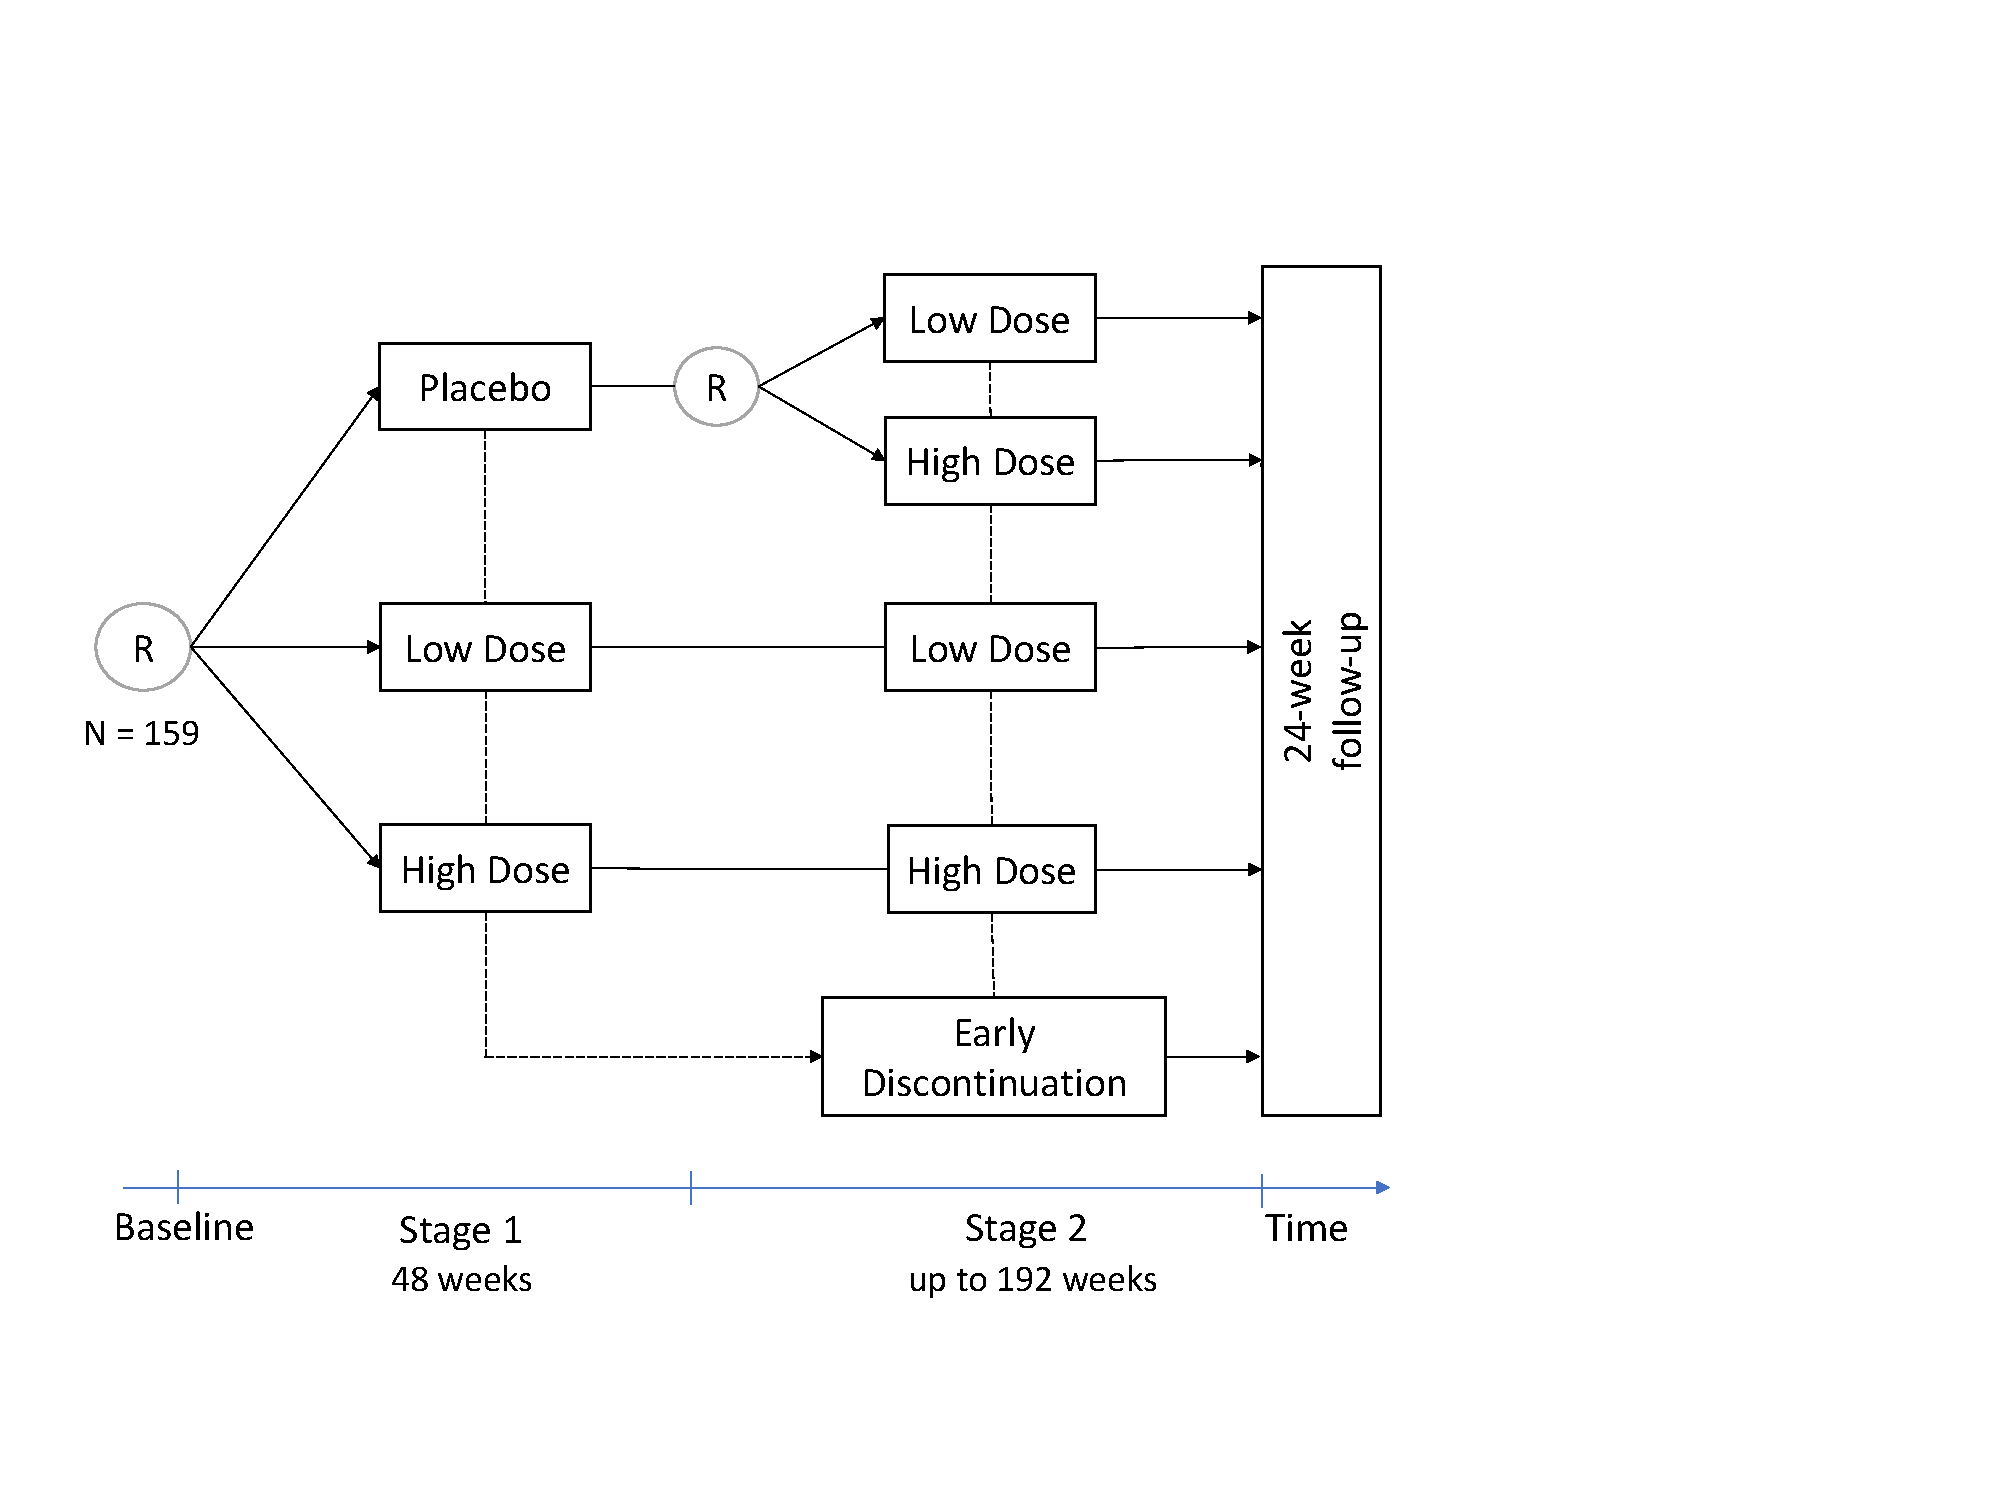
\includegraphics[width=12cm]{chapters/figures/NCT0303design.pdf}}
\\
\subfloat[]{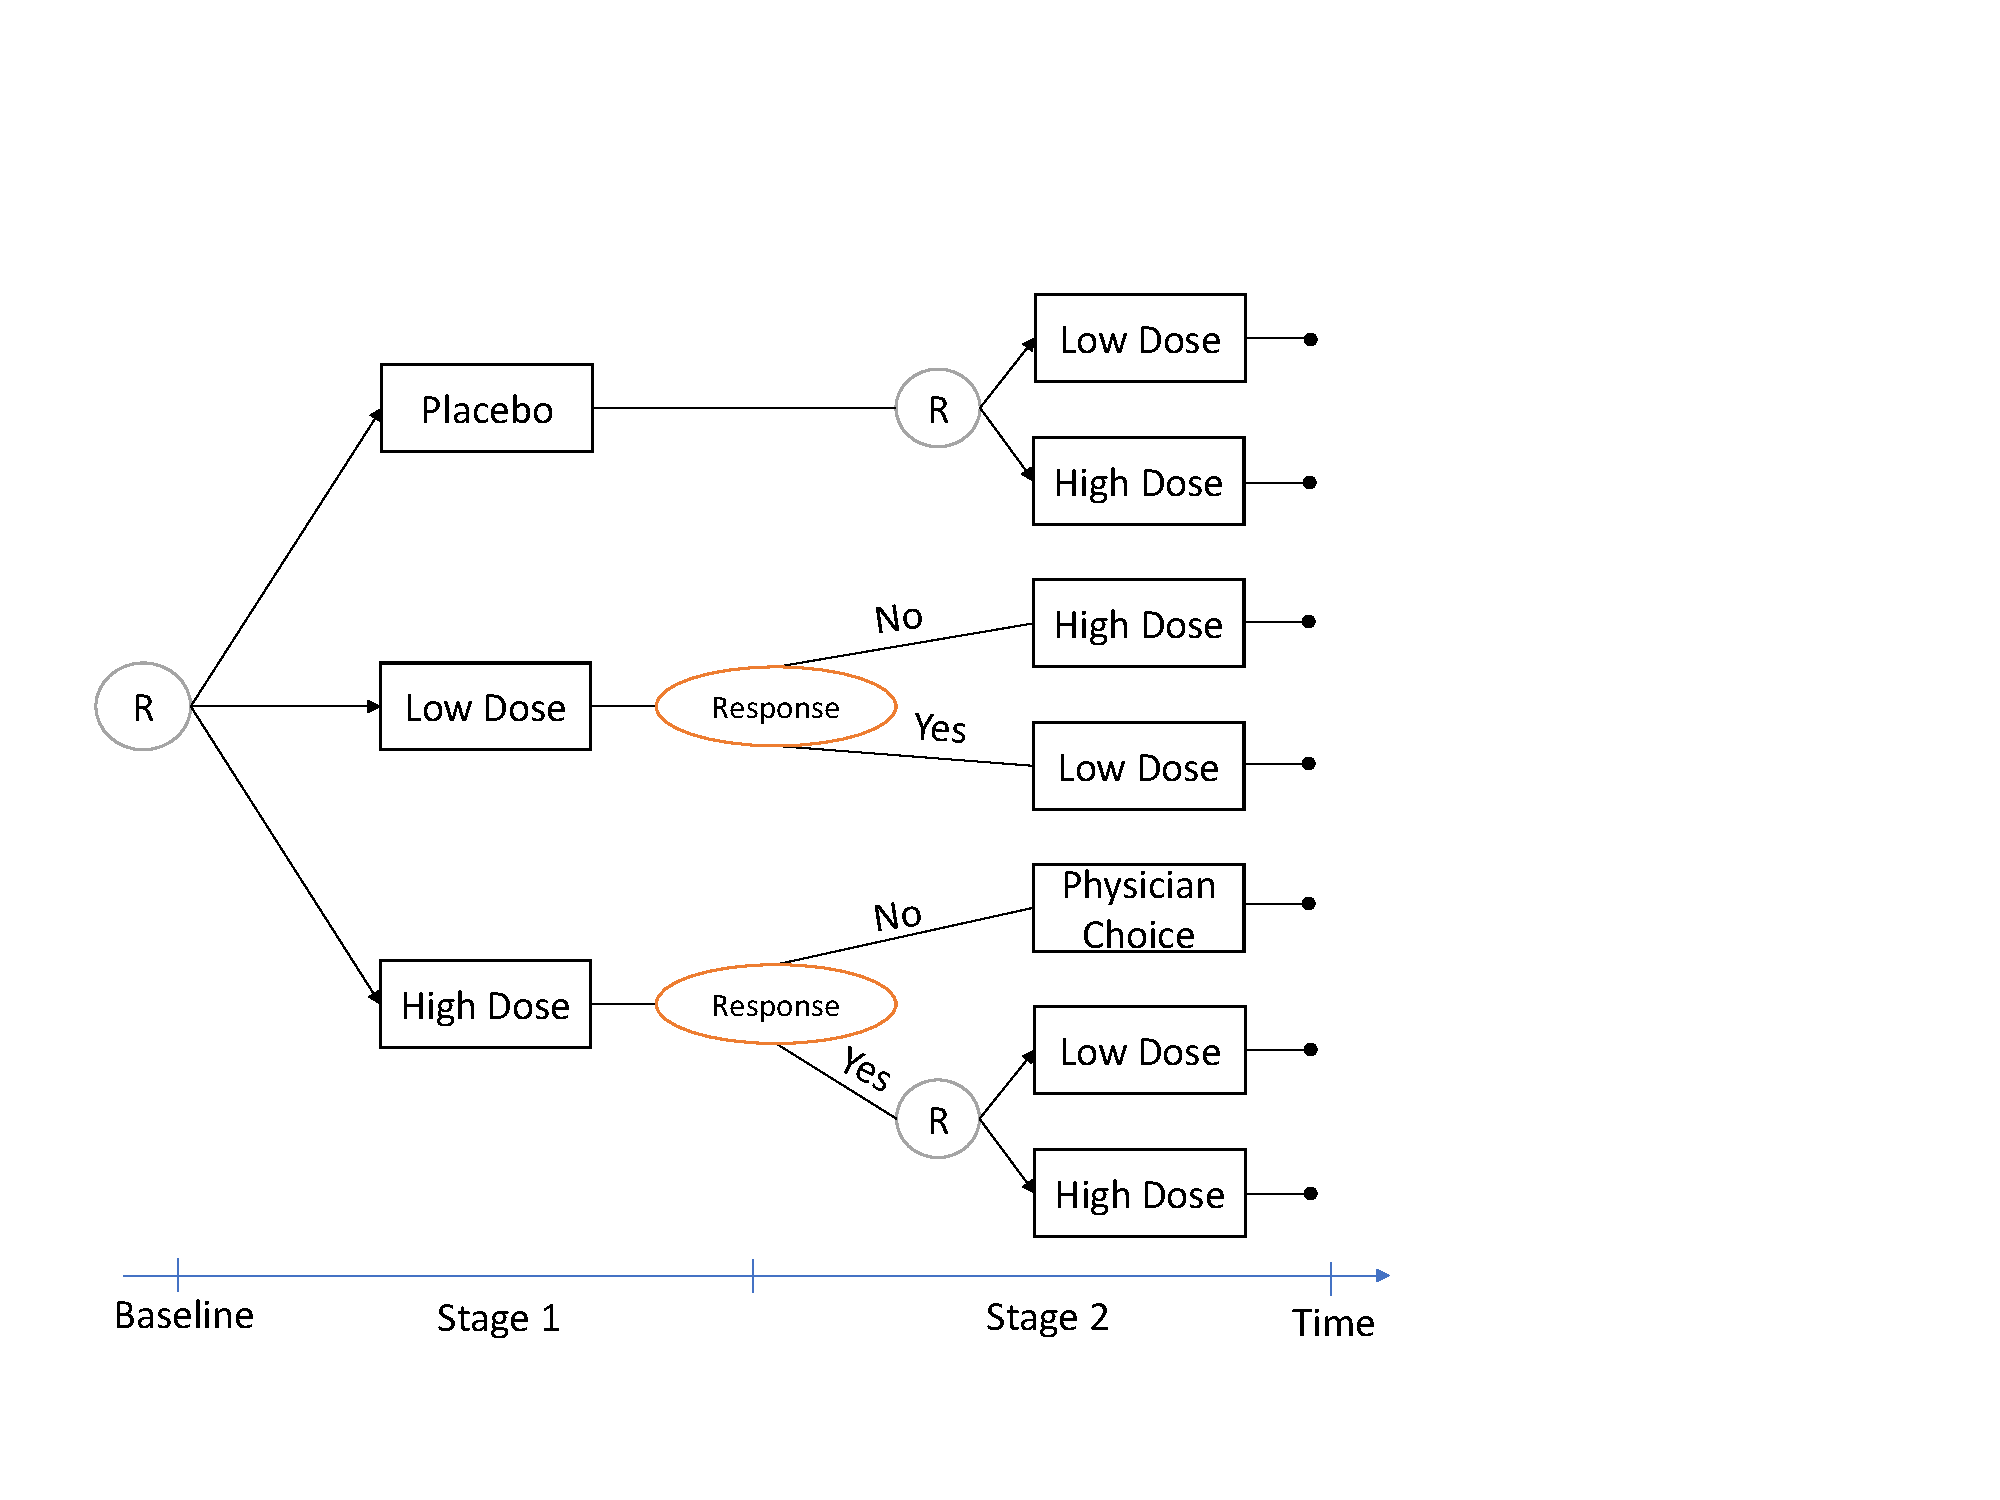
\includegraphics[width=12cm]{chapters/figures/trialdesign.pdf}}
\caption{(a) Study design of the SPITFIRE trial (NCT03039686). (R) denotes randomization. (b) Study design of the proposed \ac{snSMART} design that formally incorporates external control data. Participants are randomized (R) with 1:2:2 or 1:3:3 chances of receiving placebo, low dose or high dose, respectively, in stage 1. At the end of stage 1, participants are assigned or rerandomized to their stage 2 treatment based on their stage 1 treatment and response status. Outcomes are collected at the end of stage 1 and 2.}
\label{fig:codatasnSMART}
\end{figure}

The primary objective of the proposed \ac{snSMART} design is to estimate the stage 1 treatment effect through efficient use of data across both trial stages while formally incorporating external data. 

\section{Methods} \label{s:methods}
 
The following notation is used in this section. $Y_{jk}$ denotes the observed mean treatment effects (e.g., \ac{NSAA} total score) and $\theta_{jk}$ denotes the expected treatment effects for stage $j = 1, 2$ and treatment $k = p$ (placebo), $l$ (low dose), $h$ (high dose) respectively. For each sample of external control data $i = 1, 2, ..., n_c$, let $Y_i$ denote the observed mean placebo effect in external control data $i$, and let $\theta_i$ denote the expected mean placebo effect in external control data $i$. 

Now, we introduce the MAC-snSMART method to incorporate external control and information from both stages in \ac{snSMART} design while making inferences about stage 1. This provides a unified framework to incorporate ``all" relevant information for efficient treatment effect estimation. Here all relevant information includes external control information from any natural history studies or placebo arm data from previous trials, and trial data including placebo data in stage 1 and low/high dose information from stages 1 and 2.

\subsection{MAC-snSMART Method}
The primary goal of the proposed \ac{snSMART} design is to estimate the stage 1 treatment effects, $\theta_{1p}, \theta_{1l}$, and $\theta_{1h}$, which in our \ac{DMD} example are stage 1 mean \ac{NSAA} total score or mean \ac{6MWD}, and the difference in effects between each dose and placebo. To achieve this goal, we need to build a framework that facilitates dynamic borrowing between treatment effects, as shown in Figure \ref{fig:theta_diagram}. Challenges of this borrowing structure are apparent and require innovative solutions within the \ac{snSMART} context. Specifically, challenges include: a)  between-trial heterogeneity or conflict is inevitable given that the quality of external control data varies across studies, and b) under the proposed \ac{snSMART} design, selection bias is introduced due to non-randomized treatment assignments in stage 2 for participants who receive low dose in stage 1 and the participants who do not respond to stage 1 high dose. To tackle these two challenges, we propose a \ac{MAC}-snSMART approach with the following components.

\begin{figure}
\centering
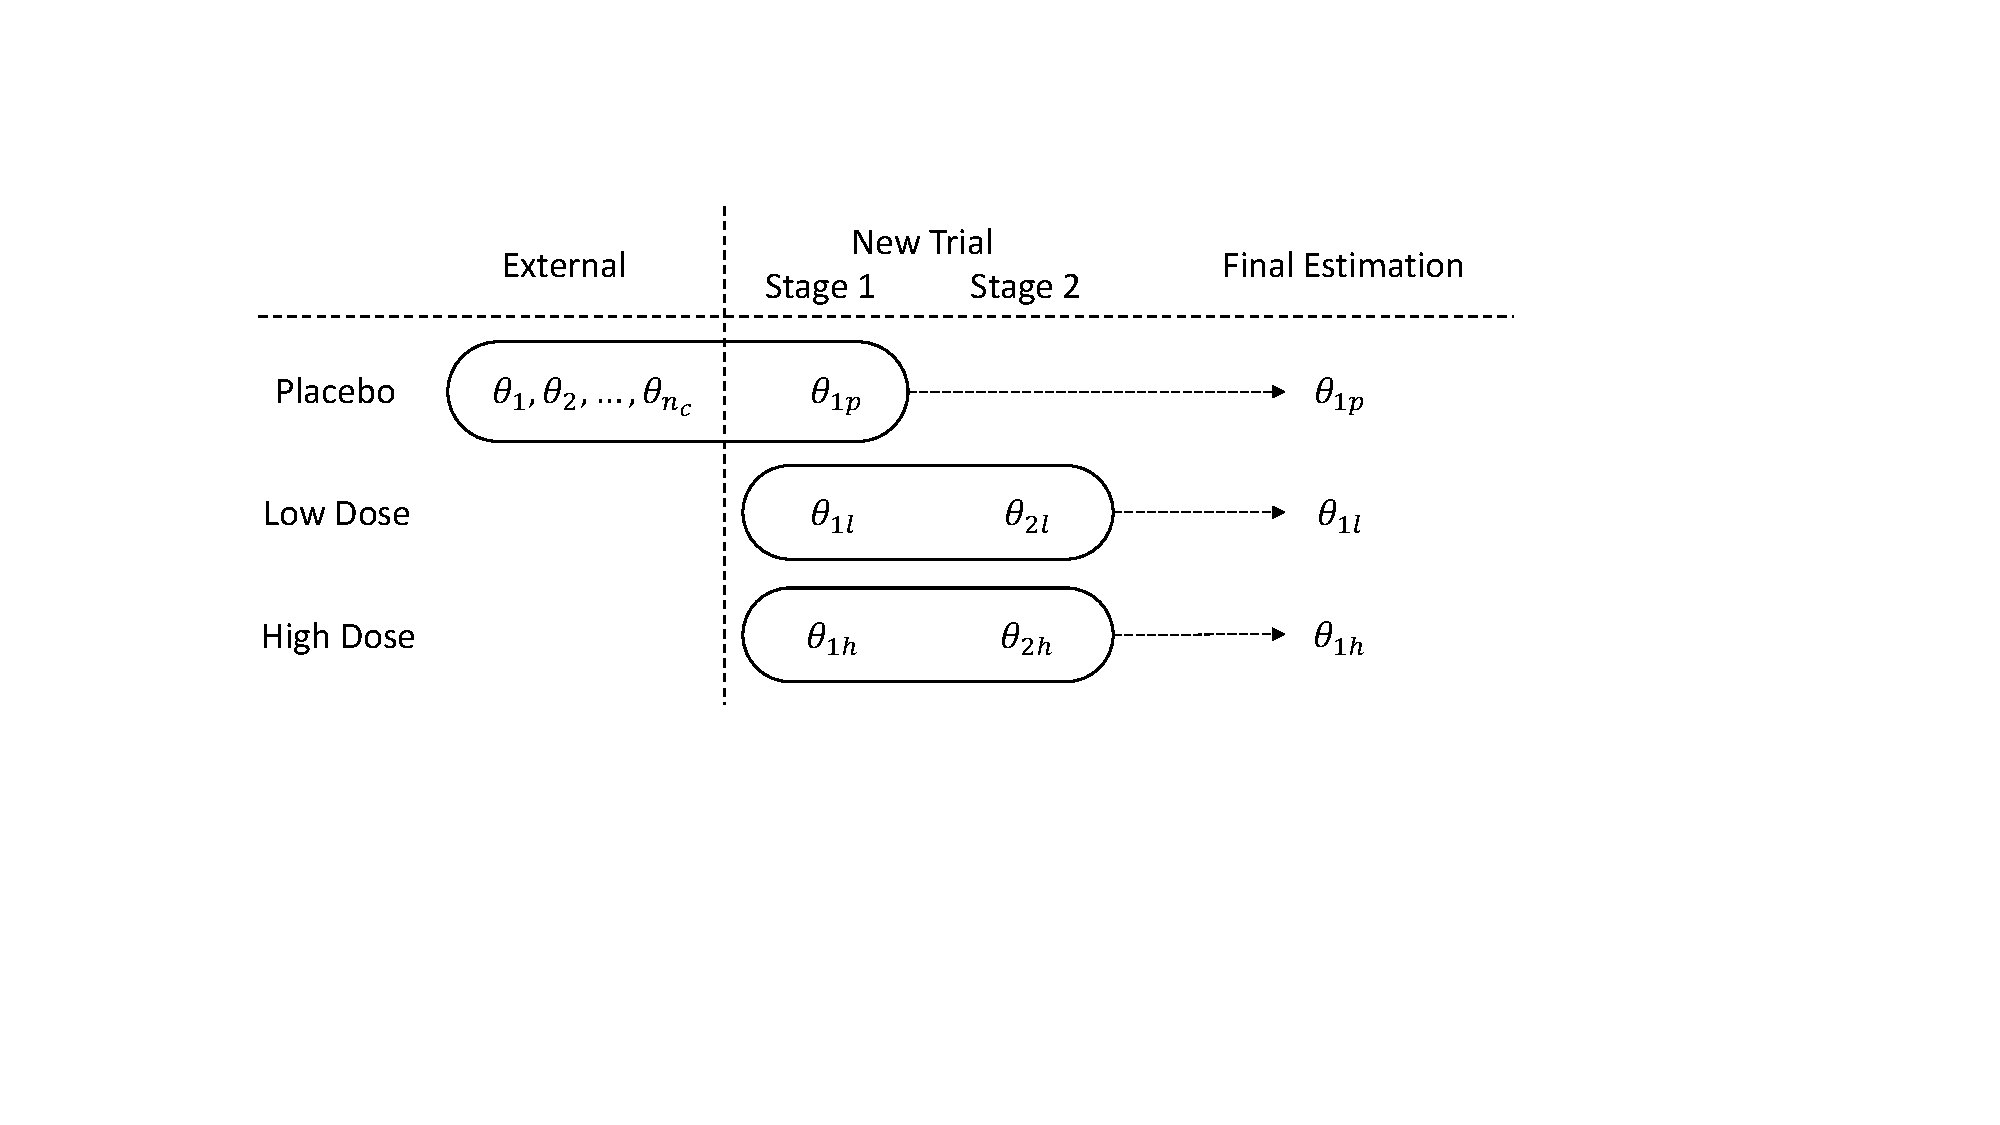
\includegraphics[width=14cm]{chapters/figures/theta_diagram.pdf}
\caption{Borrowing among treatment effects ($\theta$) in MAC-snSMART}
\label{fig:theta_diagram}
\end{figure}

\subsubsection{Combining Evidence for Placebo}
A careful selection of relevant external control data is the first critical step to control bias in the treatment effect estimate. \cite{pocock1976combination} proposed a set of criteria to assess the similarity between external control and trial control data based on the key aspects including inclusion/exclusion criteria, endpoint definition, relevance of control treatment, distribution of demographic criteria, etc. Choice of relevant external data ensures the appropriateness of the exchangeability assumption for the control parameters. Nevertheless, building a framework that acknowledges possible conflict between internal and external control is necessary to handle the effects of unmeasured confounders. 

Under the \ac{MAC}-snSMART method, $Y_i$, the observed mean placebo effect in external control data $i$, follows $Y_{i}|\theta_{i} \sim N(\theta_{i}, s_{i}^2)$, where $i = 1, 2, ...n_c$, and $s_i$ is given or derived from the $n_c$ external control data samples. Similarly, we assume $Y_{1p}|\theta_{1p} \sim N(\theta_{1p}, s_{1p}^2)$. To dynamically borrow across different studies, a parameter model is required to connect $\theta_i$ and $\theta_{1p}$. A straightforward approach to link $\theta_i$ and $\theta_{1p}$ is a hierarchical model which assumes exchangeability between internal and external control. This can be achieved by setting the same mean but a different standard deviation for each $\theta$, i.e., $\theta_{i} |\mu_p, \tau_i \sim N(\mu_p, \tau_i^2)$ and $\theta_{1p}|\mu_p,\tau_{1p} \sim N(\mu_p, \tau_{1p}^2)$. If patient-level information about important predictors is available, the model can be further extended via meta-regression. This structure accounts for external control data outliers by allowing for different between-trial standard deviations, but it could result in overly optimistic borrowing when information from different sources is non-exchangeable. 

\subsubsection{Robustification} \label{sec:robust}
To avoid overly optimistic borrowing, we include a mixture model for $\theta_i$ and $\theta_{1p}$ allowing for external control data non-exchangeability for placebo through: 
\begin{enumerate}
    \item with probability $p_{i}$, for $i = 1, 2,...,n_c$, $\theta_i|\mu_p \sim N(\mu_p, \tau_{i}^2)$; and with probability $p_{1p}$, $\theta_{1p}|\mu_p \sim N(\mu_p, \tau_{1p}^2)$
    \item with probability $1 - p_{i}$, for $i = 1, 2,...,n_c$, $\theta_i \sim N(m_i, v_i^2)$; and with probability $1 - p_{1p}$, $\theta_{1p} \sim N(m_{1p}, v_{1p}^2)$.
\end{enumerate}
A similar framework has been proposed by \cite{neuenschwander2016use}.
The prior weights $p_i$ are fixed. The values of $m_i, m_{1p}, v_i$ and $v_{1p}$ are chosen based on expert knowledge. It is essential to avoid the use of improper priors for non-exchangeability parameters ($m_{i}$, $m_{1p}$, $v_{i}$, and $v_{1p}$). Instead, weakly informative priors, such as priors worth approximately one observation \citep{kass1995reference}, should be used. 

\subsubsection{Combining Evidence for Low and High Dose Groups}

According to the proposed trial design, a participant may follow one of the seven different treatment sequences: $(1p, 2l)$, $(1p, 2h)$, $(1l, 2l)$, $(1l, 2h)$, $(1h, 2l)$, $(1h, 2h)$, and $(1h,$ \emph{No stage 2 treatment}). 
For each of the first six groups, the joint distribution of outcomes from the first and second stage, $Y_{1k}$ and $Y_{2k'}$, follows:
\begin{equation}\label{eq:joint}
\begin{bmatrix} Y_{1k} \\ Y_{2k'} \end{bmatrix} \sim MVN\left(\\ \begin{bmatrix} \theta_{1k} + b \\ \theta_{2k'}\end{bmatrix}, \begin{bmatrix} s_{1k}^2 & s_{kk'}s_{1k}s_{2k'}\\ s_{kk'}s_{1k}s_{2k'} & s_{2k'}^2\end{bmatrix}\right),
\end{equation}   
where $k = p, l, h; \ k' = l, h$. Note, $b$ is a bias correction term, which is used to adjust for the selection bias issue discussed above and further defined below. $s_{jk}$ can be estimated based on observed data in the current \ac{snSMART}. $s_{kk'}$ denotes the correlation between stage 1 treatment $k$ outcomes and stage 2 treatment $k'$ outcomes. 

Under the \ac{MAC}-snSMART approach, the conditional distribution of $\theta_{jk}$ follows that:
\begin{equation}\label{eq:theta}
   \theta_{1k},\theta_{2k} \sim N(\mu_k, \tau_k^2); \quad k = l, h \\
\end{equation}
given that we assume stage 1 and stage 2 expected outcomes for the same treatment follow the same normal distribution. Here, we explicitly define the bias correction term $b$ as:
\begin{equation}
b = I(k = l, k' = l)b_{ll} - I(k = l, k' = h)b_{lh} - I(k = h)b_{h}.
\end{equation}
Explicitly, $b_{ll}$ denotes the expected difference between the stage 1 mean treatment effect of group $(1l, 2l)$ and the overall stage 1 low dose mean treatment effect, $b_{lh}$ denotes the expected difference between the stage 1 mean treatment effect of group $(1l, 2h)$ and the overall stage 1 low dose mean treatment effect, and similarly, $b_h$ denotes the expected difference between the stage 1 mean treatment effect of high dose responders and the overall stage 1 high dose mean treatment effect. $B_{ll}, B_{lh}$ and $B_h$, the observed differences corresponding to $b_{ll}, b_{lh}$ and $b_h$, follow normal distributions $N(b_{ll}, \xi_{ll}^2)$, $N(b_{lh}, \xi_{lh}^2)$ and $N(b_h, \xi_{h}^2)$, respectively. 

\subsubsection{Prior Specification}
We suggest weakly informative normal distributions as priors for $\mu_p$ and $\mu_{k}$, weakly informative uniform distributions or normal distributions as priors for $b_{ll}, b_{lh}$ and $b_h$, and weakly informative $Unif(-1,1)$ prior distributions for $s_{kk'}$.

Half-normal priors with standard deviations roughly equal to $s_i/2$, $s_{1p}/2$ and $s_{jk}/2$ for $\tau_i$, $\tau_{1p}$ and $\tau_k$, respectively, are used to cover very small to large between-trial heterogeneity \citep{spiegelhalter2004bayesian}. According to the bias-corrected meta-analysis model proposed by \cite{verde2021bias}, roughly four participants worth of information is provided by the priors of the bias parameter. Hence, we recommend half-normal priors with standard deviation roughly equal to $s_{1l}/4, s_{1l}/4$ and $s_{1h}/4$ for $\xi_{ll}, \xi_{lh}$ and $\xi_h$, respectively. Then, the treatment effects of low dose in stage 1 and stage 2 follow the same normal distribution and are therefore exchangeable. Similarly, the high dose treatment effects in stages 1 and 2 are exchangeable.

\subsection{Posterior Distribution}
The mixture model introduced in Section \ref{sec:robust} is a mixture of normal priors. For $\theta_{1p}$, we have:
\begin{equation*}
    f(\theta_{1p}|p_{1p}, \mu_{p},\tau_{1p}, m_{1p}, v_{1p}) = p_{1p}N(\theta_{1p}|\mu_p,\tau_{1p}^2)+(1-p_{1p})N(\theta_{1p}|m_{1p},v_{1p}^2) 
\end{equation*}

Given that only summary-level treatment effect $Y_{1p}$ is used to conduct Bayesian inference, the likelihood function is the same as above. Here, we introduce the latent variable $Z_{1p}$, such that $\theta_{1p}|Z_{1p} = 1 \sim N(\mu_{p},\tau_{1p}^2)$, $\theta_{1p}|Z_{1p} = 0 \sim N(m_{1p}, v_{1p}^2)$
and $P(Z_{1p} = 1) = p_{1p}$, $P(Z_{1p} = 0) = 1-p_{1p}$.
Therefore, $Z_{1p}$ provides the label indicating the mixture components from which the observations have been generated. Now the posterior probability that $\theta_{1p}$ has been generated from $N(\mu_p, \tau_{1p}^2)$ is:
\begin{equation*}
    P(Z_{1p} = 1|\theta_{1p}, \mu_{p},\tau_{1p}, m_{1p}, v_{1p})=\frac{p_{1p}N(\mu_p, \tau_{1p}^2)}{p_{1p}N(\mu_p, \tau_{1p}^2)+(1-p_{1p})N(m_{1p}, v_{1p}^2)}.
\end{equation*}
Similarly, we could create latent variables $Z_i$ for $\theta_i$, where $i = 1, 2, ... n_c$, and use the same structure as above to obtain the posterior probability that $\theta_i$ has been generated from $N(\mu_p, \tau_i^2)$. 

Based on conjugate priors, the posterior distribution of $\theta_i$ and $\theta_{1p}$ are mixtures of normal distributions. Specifically, for $\theta_{1p}$, when equation \ref{eq:joint} is not considered, the posterior mean is:
\begin{equation*}
    p_{1p}(\eta_{1p}\hat{\mu}_p+(1-\eta_{1p})Y_{1p})+(1-p_{1p})\frac{m_{1p}(s_{1p}^2+\tau_{1p})+Y_{1p}v_{1p}^2}{s_{1p}^2+\tau_{1p}+v_{1p}^2}
\end{equation*}
where $\hat{\mu}_p = (\omega_{1p}Y_{1p} + \sum_{i}{\omega_{i}Y_{i}})/\omega_{sum}$ is the posterior mean of $\mu_p$, $\omega_i = (s_i^2+\tau_i^2)^{-1}$ and $\omega_{1p} = (s_{1p}^2+\tau_{1p})^{-1}$ are inverse variance weights, $\omega_{sum}$ is the sum of all inverse variance, and $\eta_{1p}=s_{1p}^2/(s_{1p}^2+\tau_{1p})$. 

The amount of information borrowed from external control data or second stage while estimating the treatment effects for control, low, and high dose groups can be quantified. This amount of borrowed information is sometimes expressed as effective sample size (ESS). In this manuscript, we use the expected local-information-ratio, which fulfills a basic predictive consistency requirement, as introduced by \cite{neuenschwander2020predictively}. 

\subsection{Bayesian Joint Stage Model}
The \ac{BJSM} for an \ac{snSMART} with placebo and dose levels when outcomes are continuous \citep{fang2022comparing} is an alternative way of analyzing our proposed \ac{snSMART} design. However, the \ac{BJSM} has not previously been presented to formally utilize external data. To incorporate external control data into the \ac{BJSM}, we need to calculate the effective sample size of the external control data first, then set the normal prior for the placebo treatment effect in the \ac{BJSM} to have the same effective sample size. Although the \ac{BJSM} method proposed by \cite{fang2022comparing} is designed to analyze data generated through a slightly different \ac{snSMART} design (i.e., low dose responders and non-responders are randomized and high dose non-responders continue high dose), the method itself is flexible with the number of patients on each treatment arm and the stage 2 treatment assignment rules. 
\subsection{Traditional Analytic Method}
We define a traditional analytic method for illustration purposes which mimics the method used by current, similar studies. A more traditional analytic method excludes external control data and uses only the stage 1 outcomes to estimate the stage 1 treatment effect. The SPITFIRE trial used this analytic plan to estimate the treatment effect of RO723936. Under the \ac{snSMART} design, a traditional analytic plan is structured as:
\begin{equation}\label{eq:indwo}
\begin{array}{l}
Y_{1k}|\theta_{1k} \sim N(\theta_{1k}, s_{1k}^2); \quad  k = p, l, h \\
\theta_{1k} \sim N(\mu_{1k}, \tau_{1k}^2); \quad k = l, h. \\
\end{array}
\end{equation}
Flat priors are used for $\mu_{jk}$ and $\tau_{jk}$. Other prior distributions are the same under both the robust \ac{MAC}-snSMART method and traditional method.

\section{Simulation Settings} \label{s:simulation}

We assess the sensitivity of our proposed \ac{MAC}-snSMART method to various data generating settings, possible treatment effects, exchangeability of external control data with current \ac{snSMART} data, and sample sizes. We assess two different data generation processes, one of which represents an ideal setting where data generation matches our exchangeable analytic model, and the other represents a less desirable setting where the assumption of exchangeability is violated. The first data generation process follows the assumption of the \ac{MAC}-snSMART so that $\theta_{1k}$ is set to a predetermined treatment effect and $\theta_{2k}$ is randomly generated from $N(\mu_k, \tau_k^2)$, where $\mu_k = \theta_{1k}$ and $\tau_k = 1$. Thus, the stage 1 treatment outcomes are generated based on $N(\theta_{jk}, s_{jk}^2)$ where $s_{jk} = 2$ and the stage 2 outcomes are randomly generated according to formula \ref{eq:joint}, and $s_{kk'}$ is randomly chosen within a certain range, i.e., $s_{pl} \in (-0.20, 0.20), s_{ph} \in (-0.15, 0.15), s_{ll} \in (0.70, 1), s_{lh} \in (-0.50, 0), s_{hl} \in (-0.30, 0.30)$, and $s_{hh} \in (0.70, 1)$. The second data generation process violates the assumptions of the \ac{MAC}-snSMART so that that there is no hierarchical structure (i.e., no $\mu_k$ is simulated) and $\theta_{1k}$ and $\theta_{2k}$ are not exchangeable. We set $\theta_{1k}$ to a predetermined treatment effect, and let $\theta_{2k} = \theta_{1k} + 1$. Formula \ref{eq:joint} is again used to randomly generate stage 1 and stage 2 treatment outcomes. This type of data may result from an \ac{snSMART} where a washout period between the first and second stage is inadequate. 

In addition to testing different data generation processes, we investigate the performance of our proposed models considering four treatment effect scenarios. Here, considering the \ac{DMD} context, we use a walking distance of four meters as the threshold for categorizing responders and nonresponders at the end of the stage 1. In scenario 1, we assume that the drug of interest is ineffective so that the treatment effects of placebo, low dose, and high dose are all equal to zero ($\theta_{1p} = \theta_{1l} = \theta_{1h} = 0$). In scenario 2, we assume that only the high dose is effective such that the treatment effects of placebo and low dose are zero, but high dose has a larger effect ($\theta_{1p} = \theta_{1l} = 0 < \theta_{1h} = 6$). In scenario 3, we assume that low dose has a small, but not clinically meaningful treatment effect and high dose has a clinically meaningful treatment effect ($\theta_{1p} < \theta_{1l} = 2 < \theta_{1h} = 6$). In scenario 4, we assume that low dose has a clinically meaningful effect, as does high dose ($\theta_{1p} = 0 < \theta_{1l} = 4 < \theta_{1h} = 8$). In the last scenario, to assess the sensitivity of our model to the alignment of external control and current data, we allow for $\theta_i \ne \theta_p$ for some $i$. 

Under each data generating process, 10,000 realizations per scenario were simulated. Each realization includes five sets of summary-level (mean and standard deviation) external control data (i.e., natural history of disease) and one current \ac{snSMART} dataset. Estimations from two \ac{MAC}-snSMART methods, i.e., \ac{MAC}-snSMART and robust \ac{MAC}-snSMART, and the traditional analytic method are compared. We calculate the coverage rate, \ac{rMSE}, bias, and width of the 95\% \ac{CI} of each estimator. The results section of this paper focuses on simulation results with a total sample size of 50, where 10 subjects are randomized to placebo, 20 subjects are randomized to low dose, and 20 subjects are randomized to high dose in stage 1, but results for total sample sizes of 25 are also provided in the figures.

The 95\% \ac{CI} are the narrowest intervals that include 95\% of the posterior distribution of $\theta_{jk}$, $j=1,2$, $k=p,l,h$. From scenario 1, where $\theta_{1p} = \theta_{1l} = \theta_{1h} = 0$, we define the type I error by calculating the probability that the credible intervals of $\hat{\theta}_{1l} - \hat{\theta}_{1p}$ and $\hat{\theta}_{1h} - \hat{\theta}_{1p}$ do not include 0. Similarly, from scenarios 3, 4 and 5, where the treatment effects of low and high dose are different from the treatment effect of placebo, we define power by calculating the probability that the credible intervals of $\hat{\theta}_{1l} - \hat{\theta}_{1p}$ and $\hat{\theta}_{1h} - \hat{\theta}_{1p}$ do not include 0. Model parameters are estimated via the R function jags in R package rjags \citep{rjags}.

\section{Results} \label{s:results}

For the data generation process where assumptions of exchangeability are upheld (data generating process 1), the \ac{rMSE}, bias, coverage rate, and \ac{CI} width for estimators of the expected treatment effects are shown in Figures \ref{fig:rMSE},  \ref{fig:CR}, and \ref{fig:Width}, respectively. The estimators from the \ac{MAC}-snSMART methods have smaller rMSEs than the traditional method. \ac{MAC}-snSMART methods provide similar coverage compared with the traditional method while having smaller 95\% \ac{CI} width. Even though \ac{MAC}-snSMART methods have slightly higher biases, the biases of both approaches are negligible. 
\begin{table} 
\begin{center}
\caption{\label{tab:TypeI} Simulated type I error}
\begin{tabular}{ccccccc}
\hline
\centering \multirow{2}{*}{Sample Size} & \multicolumn{2}{c}{Traditional} & \multicolumn{2}{c}{MS} & \multicolumn{2}{c}{RMS}\\
\centering  & Low & High & Low & High & Low & High \\
\hline
\textit{data generating process 1} &&&&&& \\
\raggedleft $n_{1p} = 10, n_{1l} = 20, n_{1h} = 20$ & 0.0599 & 0.0611  & 0.0452 & 0.0256 & 0.0468 & 0.0304 \\
\raggedleft $n_{1p} = 5, n_{1l} = 10, n_{1h} = 10$ & 0.0793 & 0.0745 & 0.0634 & 0.0324 & 0.0700 & 0.0374 \\
\textit{data generating process 2} &&&&&& \\
\raggedleft $n_{1p} = 10, n_{1l} = 20, n_{1h} = 20$ & 0.0664 & 0.0650 & 0.0714 & 0.0667 & 0.0730 & 0.0712 \\
\raggedleft $n_{1p} = 5, n_{1l} = 10, n_{1h} = 10$ & 0.0741 & 0.0749 & 0.0747 & 0.0569 & 0.0787 & 0.0606\\
\hline
\end{tabular}
\end{center}
\begin{tablenotes}
      \small
      \item The type I error of all presented methods is defined as the probability that the credible intervals of $\hat{\theta}_{1l} - \hat{\theta}_{1p}$ and $\hat{\theta}_{1h} - \hat{\theta}_{1p}$ do not include 0 when there are no treatment effect differences between low dose and placebo and high dose and placebo. Data generating process 1 generates datasets under the assumption that the expected treatment effect of the same dose level follows the same normal distribution across stages, and data generating process 2 generates datasets without a hierarchical structure or exchangeability between stages. $n_{1p}$, $n_{1l}$ and $n_{1h}$ denote the number of participants randomized to placebo, low dose and high dose, respectively, in stage 1. Two hierarchical models: MAC-snSMART (MS) and robust MAC-snSMART (RMS) are compared against the traditional method. 
\end{tablenotes}
\end{table}

A comparison of all metrics between the traditional method and the \ac{MAC}-snSMART methods clearly shows that estimation of the placebo effect is improved from including external control data, even when external control data is not entirely aligned with the placebo data in the current \ac{snSMART} ($\theta_{i} \ne \theta_p$ for some $i$). The robust \ac{MAC}-snSMART and the \ac{MAC}-snSMART methods provide similar estimates for low and high dose, but when external control data is not aligned with the current trial data, the placebo effect estimate is less biased under the robust \ac{MAC}-snSMART method.  

Given that stage 1 treatment outcomes are simulated with the same $n$ and the same standard deviation across scenarios with no previous treatment impact, the estimators provided by the traditional method have more stable performance across scenarios. This is in contrast to the fluctuation of metrics of the estimators provided by \ac{MAC}-snSMART methods due to the variations in $n$ and standard deviations of the stage 2 outcomes simulated under different treatment effect scenarios. 

The right column of Figures \ref{fig:rMSE}, \ref{fig:Bias}, \ref{fig:CR}, and \ref{fig:Width} present the \ac{rMSE}, bias, coverage rate, and \ac{CI} width for estimators of the treatment effects when data are generated without a hierarchical structure or exchangeability (data generating process 2). Given that the \ac{MAC}-snSMART methods borrow information across both stages, this data generation process where there is a shift in mean in stage 2 treatment effects, leads to larger positive biases and subsequently lower coverage rates and higher \ac{rMSE} values compared to the traditional method. The decrease in coverage rate can be mitigated by setting a larger standard deviation for the half-normal prior of $\tau_k$. The estimates produced by the traditional method are not affected by the mean shift in stage 2, given that only stage 1 data is used to estimate stage 1 treatment effects. Under this data generation setting, the traditional method provides the best treatment effect estimators among the presented methods. 

\begin{figure}
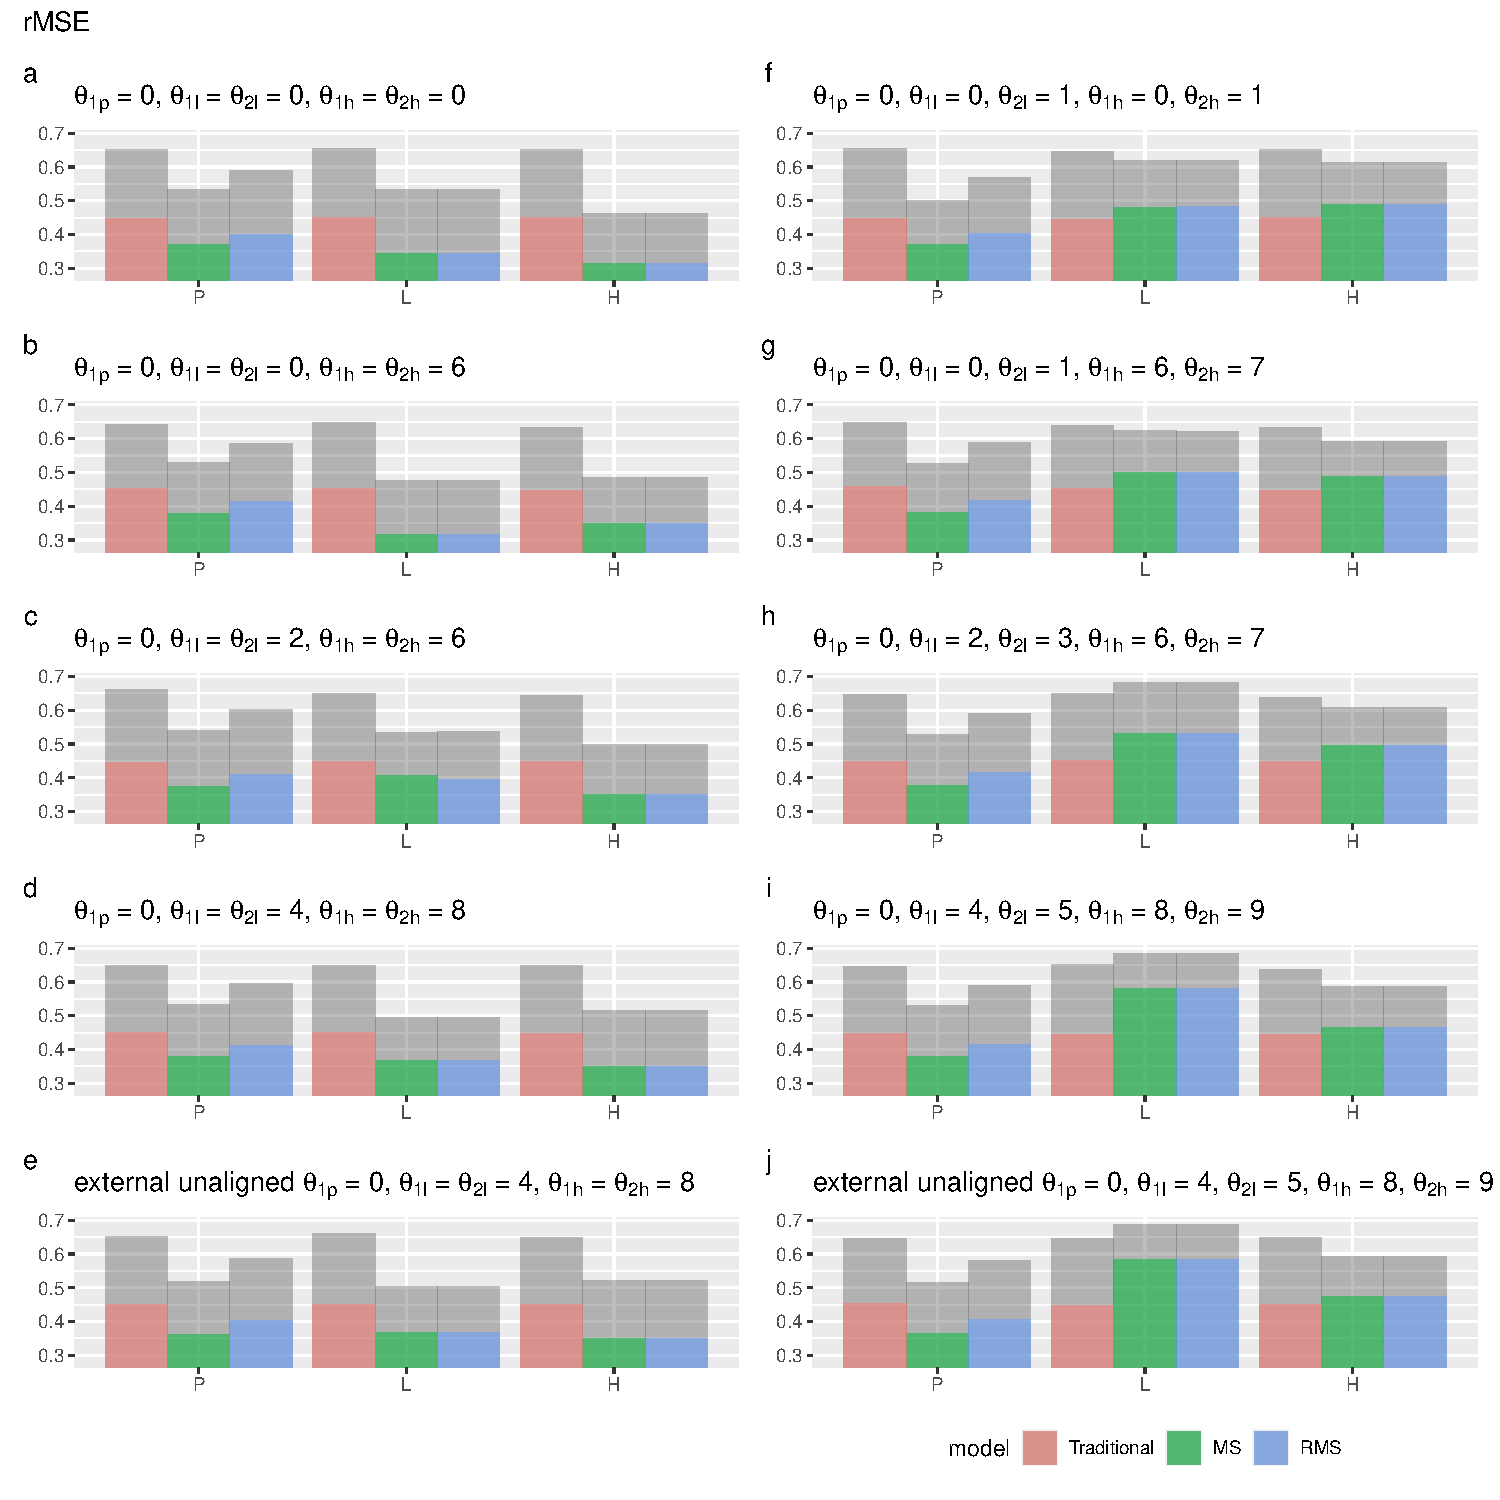
\includegraphics[width=16cm]{chapters/figures/rMSE.pdf}
\caption{Simulated root-mean-square error (rMSE) for the estimators of $\theta_{1k}$}
\subcaption*{$\theta_{jk}$ is the stage $j$ treatment effect of treatment $k$, where $j = 1,2, k = P, L, H$, P = placebo, L = low dose, and H = high dose. Two hierarchical models: MAC-snSMART (MS) and robust MAC-snSMART (RMS) methods are compared against the traditional method. The results of total sample size 50 are shown as the colored bars, while the results of total sample size 25 are shown as the overlaying grey bars. The simulation settings are described on the top of each graph, where $\theta_{jk}$ denotes the true value of the expected treatment effects of treatment $k$ in stage $j$, $j = 1, 2$, $k = P, L, H$, and \emph{external unaligned} means the placebo treatment effects in external control data are inconsistent with the placebo treatment effect in the current trial. This figure appears in color in the electronic version of this article, and color refers to that version.}
\label{fig:rMSE}
\end{figure}

\begin{figure}[H]
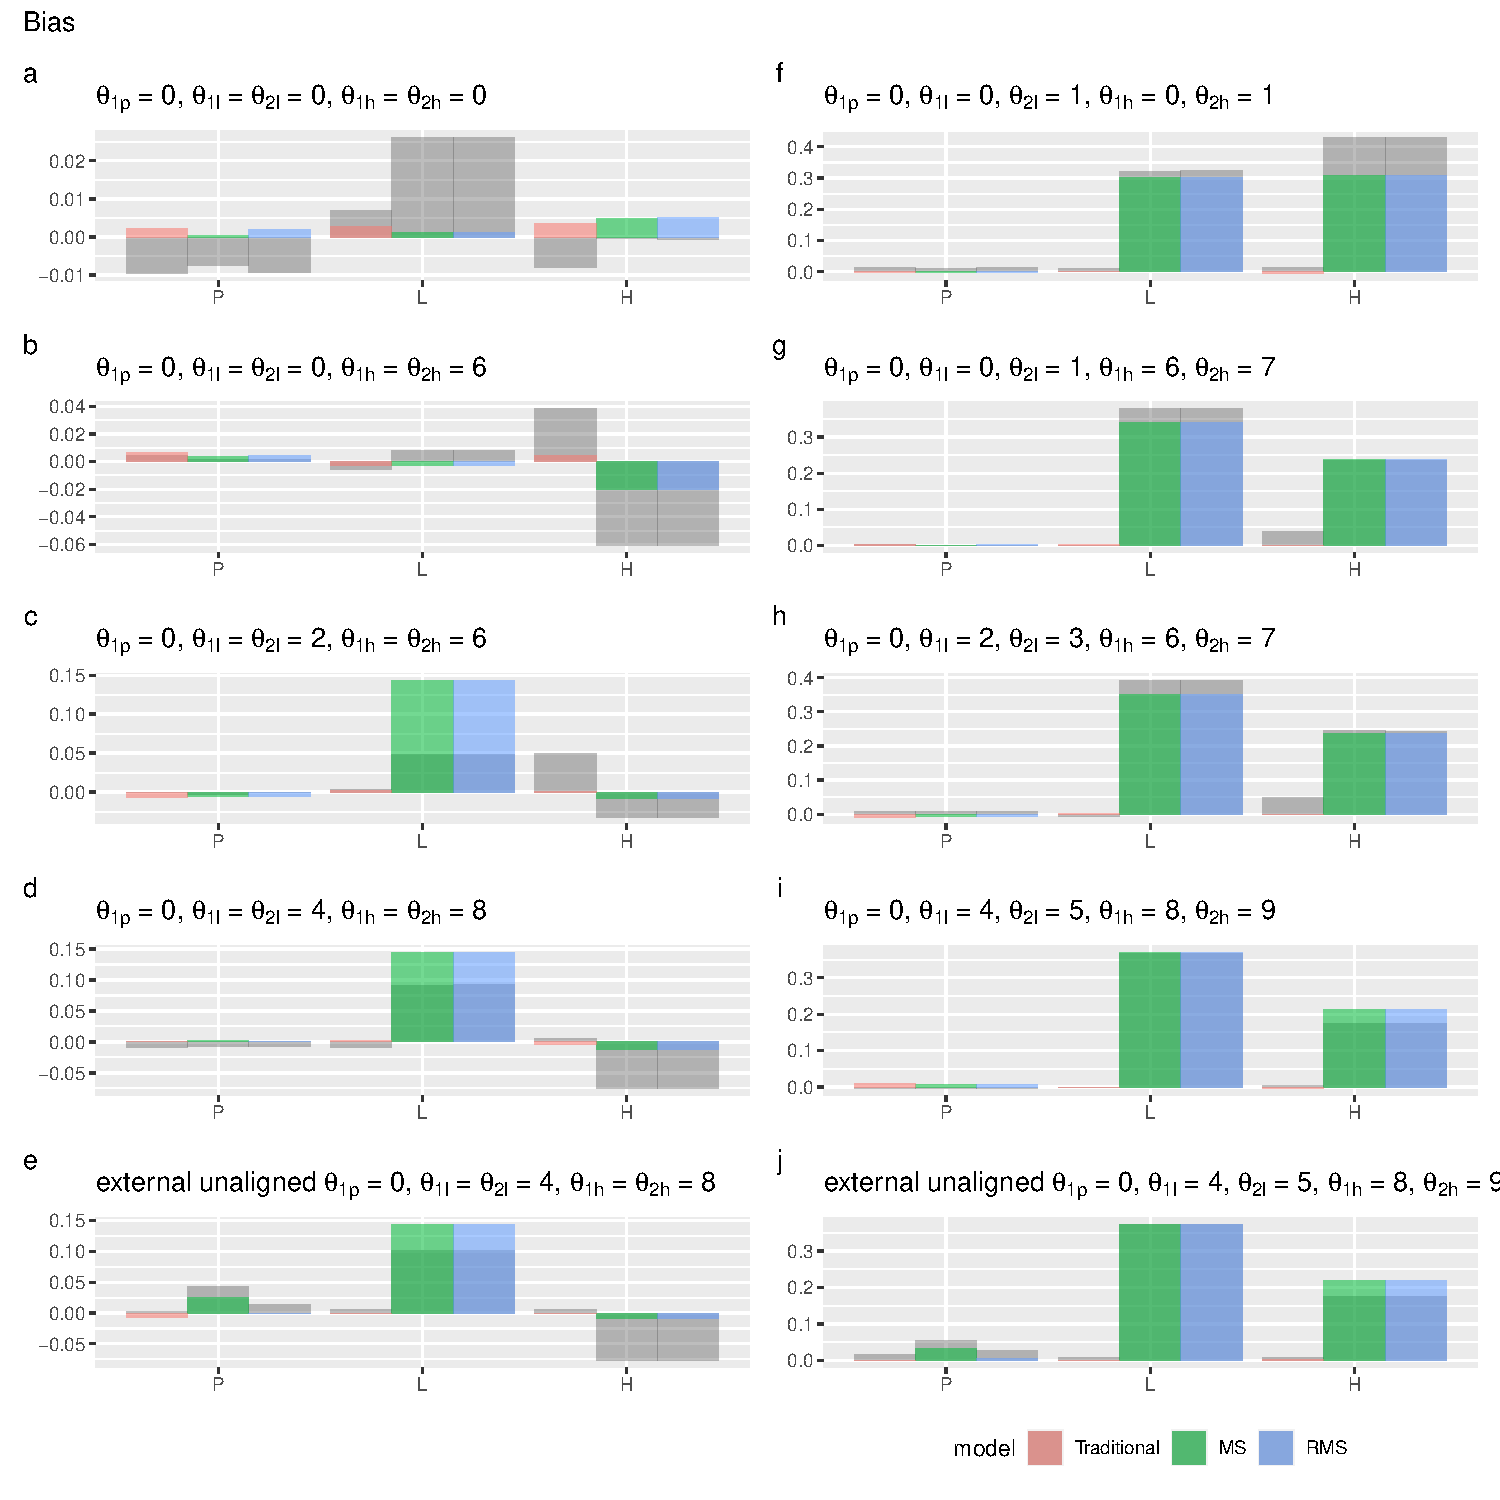
\includegraphics[width=16cm]{chapters/figures/Bias1.pdf}
\caption{Simulated bias for the estimators of $\theta_{1k}$}
\subcaption*{$\theta_{jk}$ is the stage $j$ treatment effect of treatment $k$, where $j = 1,2, k = P, L, H$, P = placebo, L = low dose, and H = high dose. Two hierarchical models: MAC-snSMART (MS) and robust MAC-snSMART (RMS) are compared against the traditional method. The results of total sample size 50 are shown as the colored bars, while the results of total sample size 25 are shown as the overlaying grey bars. The simulation settings are described on the top of each graph, where $\theta_{jk}$ denotes the true value of the expected treatment effects of treatment $k$ in stage $j$, $j = 1, 2$, $k = P, L, H$, and \emph{external unaligned} means the placebo treatment effects in external control data are inconsistent with the placebo treatment effect in the current trial.}
\label{fig:Bias}
\end{figure}

\newpage
\begin{figure}[H]
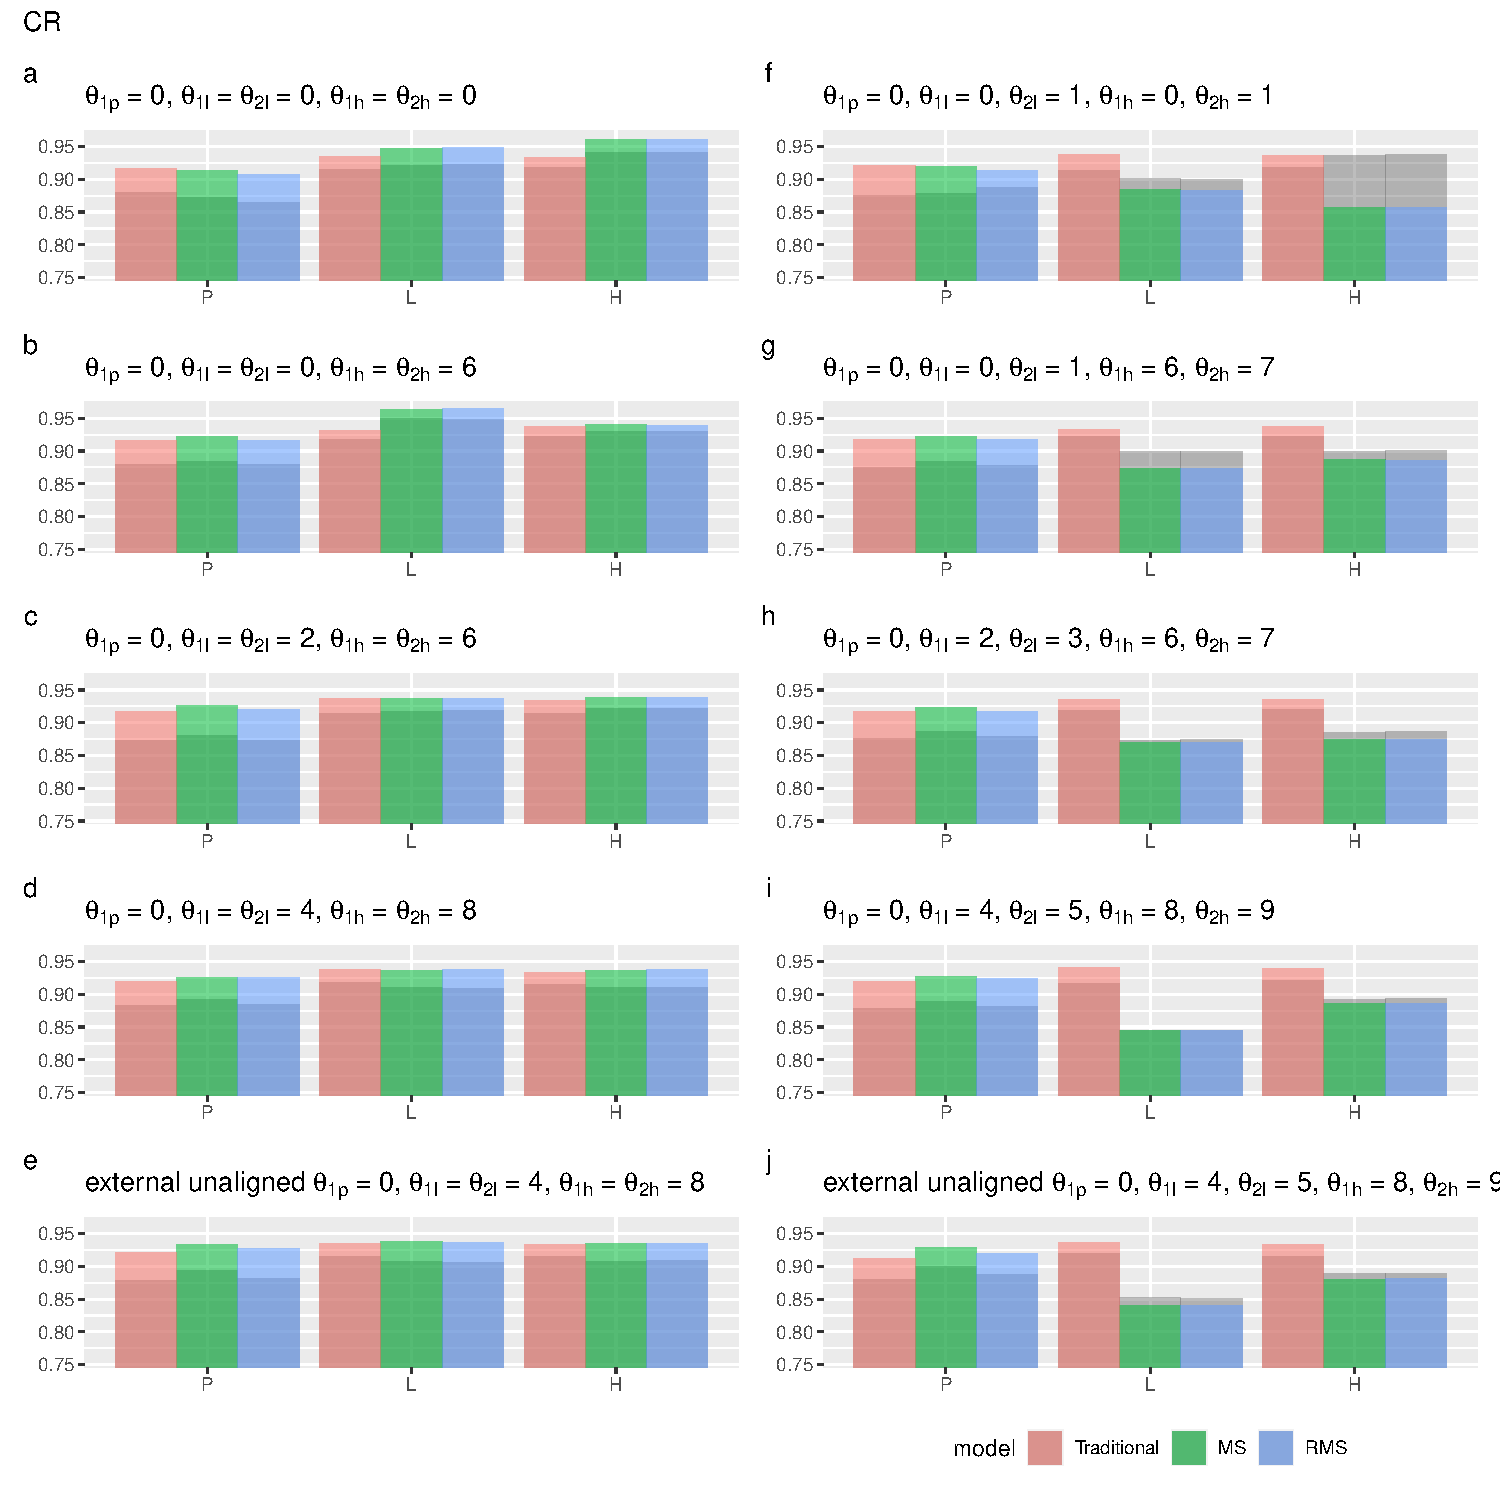
\includegraphics[width=16cm]{chapters/figures/CR.pdf}
\caption{Simulated 95\% coverage rate (CR) for the estimators of $\theta_{1k}$}
\subcaption*{Note: $\theta_{jk}$ is the stage $j$ treatment effect of treatment $k$, where $j = 1,2, k = P, L, H$, P = placebo, L = low dose, and H = high dose. Two hierarchical models: MAC-snSMART (MS) and robust MAC-snSMART (RMS) are compared against the traditional method. The results of total sample size 50 are shown as the colored bars, while the results of total sample size 25 are shown as the overlaying grey bars. The simulation settings are described on the top of each graph, where $\theta_{jk}$ denotes the true value of the expected treatment effects of treatment $k$ in stage $j$, $j = 1, 2$, $k = P, L, H$, and \emph{external unaligned} means the placebo treatment effects in external control data are inconsistent with the placebo treatment effect in the current trial.}
\label{fig:CR}
\end{figure}

\newpage
\begin{figure}[H]
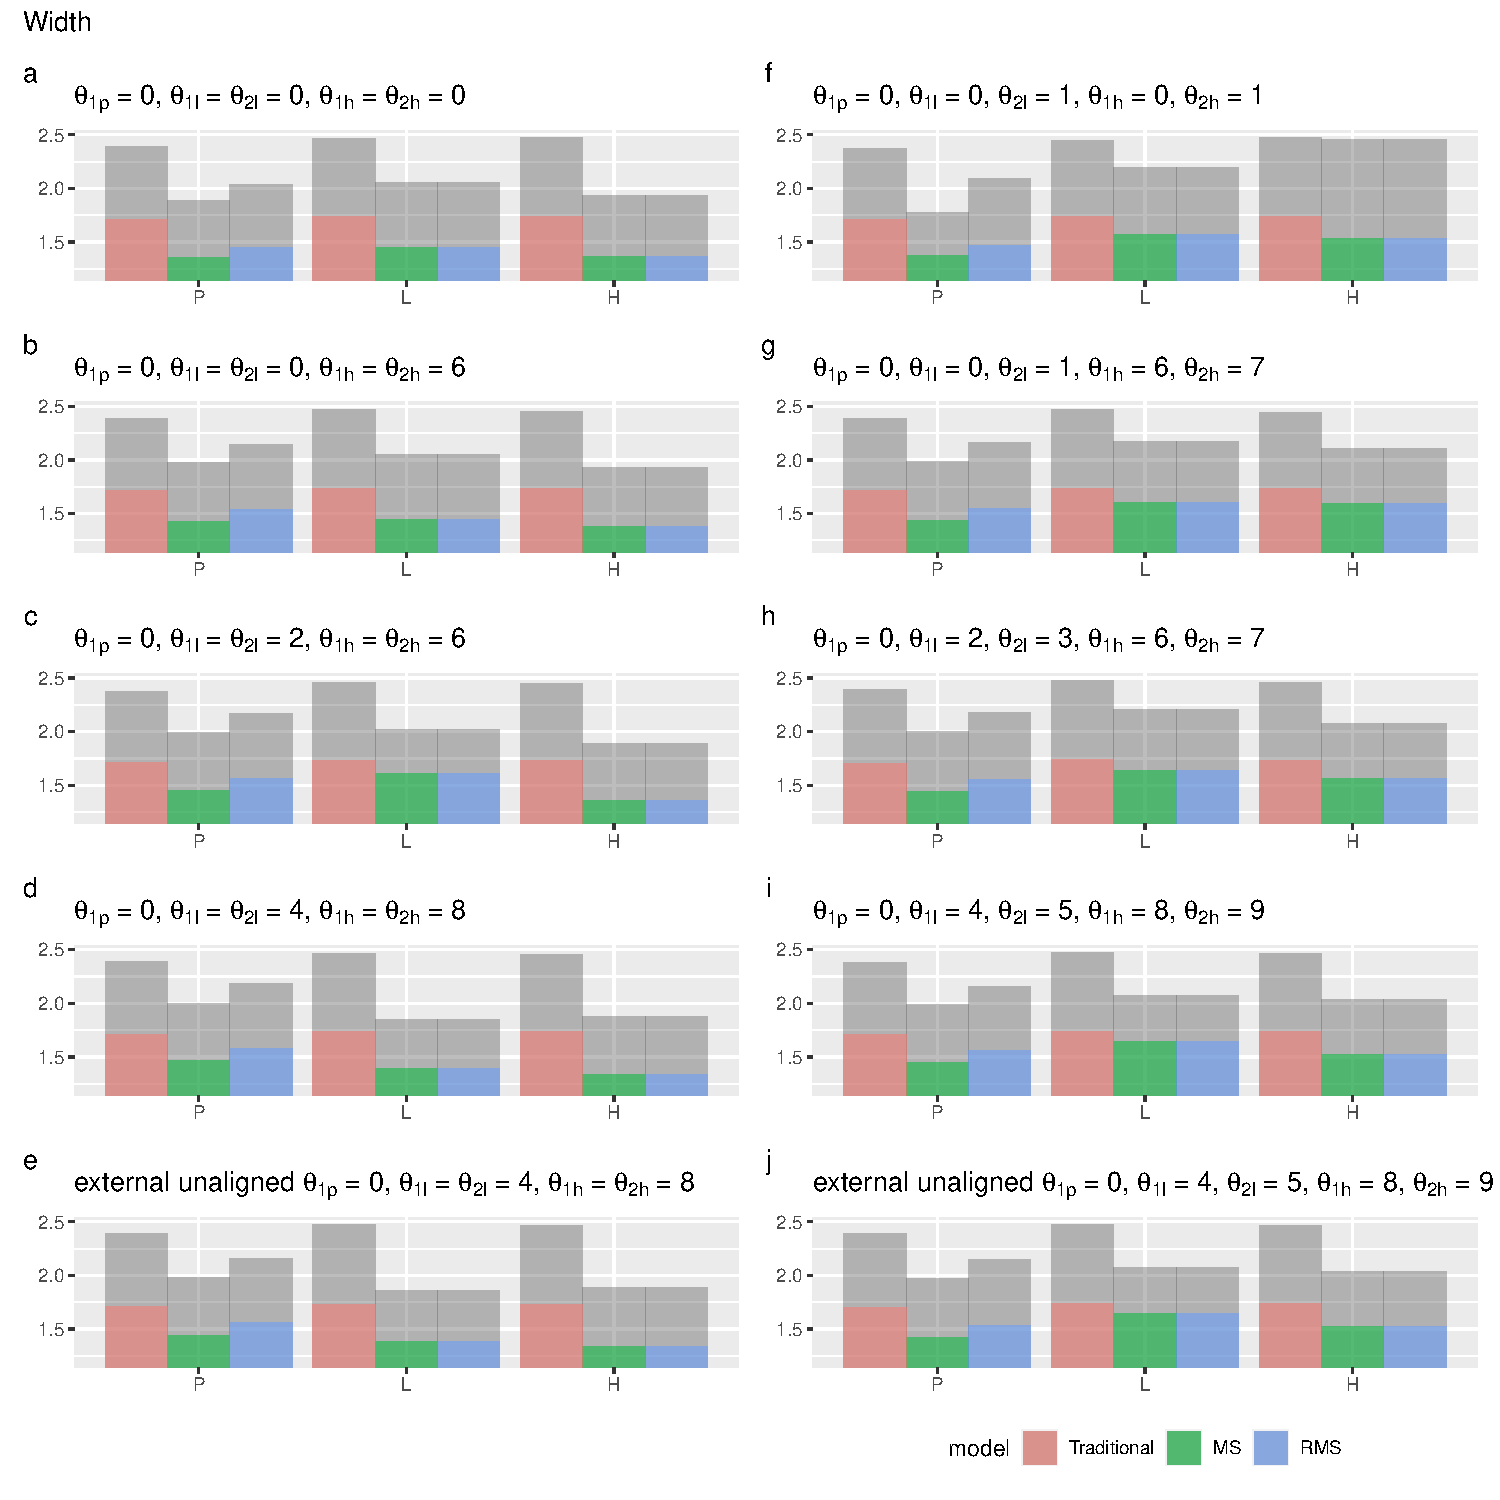
\includegraphics[width=16cm]{chapters/figures/Width.pdf}
\caption{Simulated width for the estimators of $\theta_{1k}$}
\subcaption*{Note: $\theta_{jk}$ is the stage $j$ treatment effect of treatment $k$, where $j = 1,2, k = P, L, H$, P = placebo, L = low dose, and H = high dose. Two hierarchical models: MAC-snSMART (MS) and robust MAC-snSMART (RMS) are compared against the traditional method. The results of total sample size 50 are shown as the colored bars, while the results of total sample size 25 are shown as the overlaying grey bars. The simulation settings are described on the top of each graph, where $\theta_{jk}$ denotes the true value of the expected treatment effects of treatment $k$ in stage $j$, $j = 1, 2$, $k = P, L, H$, and \emph{external unaligned} means the placebo treatment effects in external control data are inconsistent with the placebo treatment effect in the current trial.}
\label{fig:Width}
\end{figure}

Similar trends were observed in simulations with sample sizes of 25. As expected, bias, \ac{rMSE} and \ac{CI} width were larger, and coverage rate was smaller than cases where the total sample size was 50. Notably, \ac{MAC}-snSMART methods still provide negligible bias and more than 90\% coverage rate for low dose and high dose under all scenarios when assumptions are not violated. 

Table \ref{tab:TypeI} and Figure \ref{fig:Power} present the type I error and power of each model. The \ac{MAC}-snSMART methods have smaller type I errors when its assumption of full exchangeability between stages is upheld, and the type I error is still reasonable (below 0.1) when this assumption is violated. The traditional method performs best when the assumptions of \ac{MAC}-snSMART methods are violated. When the treatment effect is $\geqslant 4$, i.e., a clinically meaningful difference in our simulations, all methods have power close to 1 under all scenarios, even when the total sample size is 25. When the treatment effect is equal to 2, the \ac{MAC}-snSMART methods have an increase in power in comparison with the traditional method, especially when the total sample size is small.      

\section{Example Data Analysis} \label{s:example}

To understand the practical utility of the proposed \ac{snSMART} design and \ac{MAC}-snSMART methods, we conducted a reanalysis using the study results of SPITFIRE study. Given that the trial stopped for futility after stage 1, we were only able to obtain summary-level \ac{NSAA} total score and summary-level \ac{6MWD} at baseline and week 48 (details shown in Table \ref{tab:Roche}). To create a dataset that matches our proposed trial design, we simulated stage 1 patient-level data by randomly drawing from normal distributions based on the SPITFIRE data. Here we describe the simulation process for \ac{NSAA} total score in detail. Specifically, 30 patients' outcomes for the placebo arm were represented by drawing from $N(-2.99, 0.65^2 \times \sqrt{30})$, 29 patient outcomes for the low dose arm were represented by drawing from $N(-3.44, 0.67^2 \times \sqrt{29})$, and 33 patient outcomes for the high dose arm were represented by drawing from $N(-2.41, 0.64^2 \times \sqrt{33})$. According to the SPITFIRE study protocol, we set a change of $\geqslant -3.1$ points from baseline as the threshold for a clinically meaningful treatment effect \citep{muntoni2018minimal}. This threshold is also used to categorize stage 1 responders and nonresponders. Stage 2 treatment outcomes were again randomly generated according to formula \ref{eq:joint} with $s_{kk'}$ randomly chosen between -1 and 1, and $Y_{2l} \sim N(-3.44, 0.67^2\sqrt{n_{2l}})$ and $Y_{2h} \sim N(-2.41, 0.64^2\sqrt{n_{2h}})$, for low and high dose, respectively. Our proposed \ac{snSMART} design and randomly generated stage 1 outcomes dictated $n_{2l}$ and $n_{2h}$. We followed the same procedure to simulate stage 1 and stage 2 \ac{6MWD} data.

Given our methods formally incorporate external control data, we used the \ac{CINRG} \ac{DNHS} data as the source of external control in this real-trial motivated example data analysis. Data from participants from the \ac{DNHS} who met the eligibility criteria of the SPITFIRE trial and had \ac{NSAA} total score or \ac{6MWD} records were used for the external control group. Given that the participant visit schedule of \ac{DNHS} was different from the SPITFIRE trial, for each participant, we picked the test record with `days from baseline' closest to 336 ($48 \times 7$) as their `Week 48' record. In the end, for \ac{NSAA} total score, data from 25 participants were included in the external control group with a mean \ac{NSAA} total score change from baseline being -1.04 and its standard deviation being 0.77. Similarly, for \ac{6MWD}, data from 25 participants were included in the external control group with a mean \ac{6MWD} change from baseline being -22.36 and its standard deviation being 27.98.

\begin{table}[H]
\caption{\label{tab:Roche} The SPITFIRE trial Study Measures. Summary
statistics are reported as mean (SD) for NSAA and 6MWD.}
\begin{center}
\begin{tabular}{p{4.8cm}p{3cm}p{2.9cm}p{3cm}}
\centering  & \centering Placebo & \centering RO7239361 Low Dose & \centering RO7239361 High Dose \tabularnewline
\hline
\textit{Baseline} &&&\\
\raggedleft Sample Size & \centering 56 & \centering 55 & \centering 55 \tabularnewline 
\raggedleft NSAA & \centering 23.1  (6.4) & \centering 24.5  (5.5) & \centering 22.7  (6.7) \tabularnewline
\raggedleft 6MWD & \centering 388.33 (69.59) & \centering 399.73 (68.35) & \centering 370.73 (93.35) \tabularnewline
\hline
\textit{Week 48} &&& \tabularnewline
\raggedleft Sample Size - NSAA & \centering 30 & \centering 29 & \centering 33 \tabularnewline 
\raggedleft Changes in NSAA & \centering -2.99  (0.65) & \centering -3.44  (0.67) & \centering -2.41  (0.64) \tabularnewline
\raggedleft Sample Size - 6MWD & \centering 29 & \centering 25 & \centering 31 \tabularnewline 
\raggedleft Changes in 6MWD & \centering -41.3 (8.7) & \centering -39.6 (9.0) & \centering -30.0 (8.7) \tabularnewline
\hline
\end{tabular}
\end{center}
\end{table}

Along with the robust \ac{MAC}-snSMART method, the \ac{BJSM} method \citep{fang2022comparing} was also implemented to analyze the SPITFIRE trial data. The estimators obtained from the \ac{BJSM} are compared with the robust \ac{MAC}-snSMART estimators to see whether our model generates estimates consistent with the \ac{BJSM}.

Given that there is wide variation in outcomes, 30,000 realizations were simulated for both \ac{6MWD} and \ac{NSAA} total score to assess the model performances. We fitted the traditional analytic method, \ac{BJSM}, and robust \ac{MAC}-snSMART method, where the results are shown in Table \ref{tab:comp}. Given that the original result of the SPITFIRE trial was obtained through fitting a \ac{MMRM} and we do not have access to the covariates that were included in that \ac{MMRM} model, it is reasonable for the traditional analytic method to have estimators with slightly larger \ac{CI} width. In fact, if we manually calculate the \ac{6MWD} \ac{CI} width based on the data in Table \ref{tab:Roche} through $1.7 \pm 1.96 \times \sqrt{8.7^2 + 9.0^2}$ and $11.3 \pm 1.96 \times \sqrt{8.7^2 + 8.7^2}$, we would obtain $(-22.83, 26.23)$ and $(-12.82, 35.42)$, which are almost the same with the \ac{6MWD} \ac{CI} obtained from the traditional analytic method. The same applies to \ac{NSAA} total score. Notice that the estimators obtained from the robust \ac{MAC}-snSMART method and \ac{BJSM} are consistent with each other and have significantly smaller \ac{CI} width than the traditional method because of the efficient use of data across both stages. 

\begin{table} 
\caption{\label{tab:comp} Example Data Analysis Result Comparison}
\begin{center}
%\begin{tabular}{p{2.6cm}p{3.3cm}p{3.3cm}p{3.3cm}p{3.3cm}}
\begin{tabular}{ccccc}
Estimator &  Original Result &  Traditional &   BJSM &  RMS  \tabularnewline
\hline
\multicolumn{1}{l}{\textit{NSAA}} &&&&\\
\multicolumn{1}{r}{$\hat{\theta}_{1p}$} &  -2.99 (-4.26, -1.71) &  -2.98 (-4.24, -1.73) &  -2.91 (-4.01, -1.82) &  -2.89 (-3.68, -2.10) \tabularnewline 

\multicolumn{1}{r}{$\hat{\theta}_{1l}$}  &  -3.44 (-4.75, -2.13) &  -3.44 (-4.74, -2.14) &  -3.38 (-4.34, -2.41) &  -3.40 (-4.49, -2.31)  \tabularnewline

\multicolumn{1}{r}{$\hat{\theta}_{1h}$} &  -2.41 (-3.66, -1.16) &  -2.41 (-3.65, -1.17) &   -2.42 (-3.35, -1.48) &  -2.49 (-3.56, -1.42) \tabularnewline

\multicolumn{1}{r}{$\hat{\theta}_{1l} - \hat{\theta}_{1p}$} &  -0.45 (-2.17, 1.27) &  -0.46 (-2.27, 1.36) &  -0.46 (-1.91, 0.98) &  -0.52 (-1.88, 0.83)   \tabularnewline
\multicolumn{1}{r}{$\hat{\theta}_{1h} - \hat{\theta}_{1p}$} &  	0.58 (-1.10, 2.26) &  0.58 (-1.20, 2.35) &  0.50 (-0.93, 1.92) &  0.40 (-0.94, 1.74) \tabularnewline
\hline
\multicolumn{1}{l}{\textit{6MWD}} &&&&\\
\multicolumn{1}{r}{$\hat{\theta}_{1p}$} &  -41.3 (-58.4, -24.2) &  -41.3 (-58.2, -24.5) &  -41.1 (-54.4, -27.8) &  -41.0 (-52.5, -29.3) \tabularnewline 

\multicolumn{1}{r}{$\hat{\theta}_{1l}$} &  -39.6 (-57.2, -22.0) &  -39.6 (-57.0, -22.2) &  -39.3 (-51.6, -27.6) &  -39.4 (-53.2, -26.1)  \tabularnewline

\multicolumn{1}{r}{$\hat{\theta}_{1h}$} &  -30.0 (-47.1, -12.9) &  -30.0 (-46.7, -13.0) &   -29.7 (-40.8, -18.7) &  -30.2 (-42.1, -18.0) \tabularnewline

\multicolumn{1}{r}{$\hat{\theta}_{1l} - \hat{\theta}_{1p}$} &  1.7 (-21.1, 24.6) &  1.8 (-22.6, 26.0) &  1.8 (-16.6, 19.5) &  1.6 (-15.6, 19.1)    \tabularnewline
\multicolumn{1}{r}{$\hat{\theta}_{1h} - \hat{\theta}_{1p}$} &  11.3 (-11.0, 33.6) &  11.5 (-12.5, 35.4) &  11.4 (-5.8, 28.6) &  10.9 (-6.4, 28.1) \tabularnewline
\hline
\end{tabular}
\end{center}
\begin{tablenotes}
      \small
      \item Note: $\hat{\theta}_{1k}$ is the estimated stage 1 treatment effect for treatment $k$, $k = P,L,H$. Four analytic methods: original SPITFIRE trial results, traditional analytic method, Bayesian joint stage modeling (BJSM), and robust MAC-snSMART (RMS) are compaired. The confidence or credible intervals of the estimates are shown in the parenthesis.
\end{tablenotes}
\end{table}

\section{Discussion} \label{s:discuss}
In this paper, we were motivated by the rare disease setting of \ac{DMD} and the SPITFIRE trial to present an alternative design and methods with more efficient use of second stage data. We have proposed a robust \ac{MAC}-snSMART method to estimate the treatment effect of placebo, low and high doses from an \ac{snSMART} design with a continuous outcome of interest. Our proposed \ac{snSMART} design and robust \ac{MAC}-snSMART method are highly responsive to the \ac{FDA}'s Complex Innovative Design program \citep{fdaCID}. We have provided guidelines for prior distributions, sensitivity analyses to assumptions of the models, and comparator models which an investigator or sponsor can provide to regulatory officials to illustrate the efficiency and robustness of the robust \ac{MAC}-snSMART method for an \ac{snSMART} design. The robust \ac{MAC}-snSMART method provides the most accurate and robust estimators when the expected treatment effect of the same dose level follows the same normal distribution across stages. 

Our \ac{snSMART} design and this assumption of the robust \ac{MAC}-snSMART method that treatment effects of the same dose level follow the same normal distribution across arms is most appropriate for diseases that stay relatively stable throughout the trial period, and when there is no treatment effect, patients' primary outcomes do not fluctuate dramatically. Diseases like \ac{DMD} used as motivation here, corticobasal degeneration (CBD), and familial Mediterranean fever (FMF), which are slower to progress, are good candidates for our \ac{snSMART} design and methods. The proposed robust \ac{MAC}-snSMART method assumes treatment effects from the first and second stages are exchangeable which incorporates this assumption of a stable disease and assumes a stable treatment effect with an adequate washout period between stages 1 and 2. If first and second stage treatment effects are not similar across stages or there is not an adequate washout period, a multi-stage design and robust exchangeable model may not be appropriate and lead to biased estimation of treatment effects as we saw in the deteriorating performance of the robust \ac{MAC}-snSMART method results under the second data generation process. At the end of the trial, sensitivity analyses comparing results from the traditional analytic method can be compared to the robust \ac{MAC}-snSMART method to assess these assumptions. 

It is possible that even a high dose of the treatment being investigated cannot provide a clinically meaningful treatment effect by the end of stage 1. Under this scenario, it will not be ethical to continue the trial for those who received high dose in stage 1. Hence, we recommend that if less than 30\% of patients responded to high dose in stage 1, stage 2 will not be conducted, and all treatment effects will be calculated based on stage 1 outcome only.

The \ac{MAC}-snSMART method provides significant power gains compared to two-sample t-tests, which are commonly used in \ac{DMD} trials. For example, under simulation scenario 2 ($\theta_p < \theta_l = 2 < \theta_h = 6$), with $s_{1p} = 1.5, s_{1l} = 2, n_{1p} = 10, n_{1l} = 20$ and $\alpha=0.05$, a one-sided two-sample t-test can only achieve a power of 0.89, while our simulation shows that \ac{MAC}-snSMART methods can achieve a power higher than 0.95 (Figure \ref{fig:Power}). The power gain is even more significant in smaller samples. When $n_{1p} = 5, n_{1l} = 10$, the power of a t-test can only reach 0.62 while the power of \ac{MAC}-snSMART method can reach 0.76 (Figure \ref{fig:Power}). This demonstrates that our proposed trial design and method are useful for obtaining a higher level of evidence for efficacy in rare disease dose-finding trials.

All of our simulations adopted the 1:2:2 placebo, low dose, and high dose randomization ratio in stage 1. A randomization ratio of 1:3:3 can be used when external control data is (almost) fully exchangeable with the current trial placebo data. With a smaller proportion of participants being randomized to the placebo arm in stage 1, the external control data will have a stronger impact than the current trial placebo data on the estimation of the placebo treatment effect. 

In our simulations, we generated five sets of summary-level external control data in each realization, which may or may not be consistent with the available placebo data in a current trial. Due to between-trial heterogeneity, the amount of effective external control data information is not simply the number of external control data placebo subjects, it must be a smaller number. We see in our example data analysis that the robustified summary-level natural history data of 25 participants is roughly equivalent to an effective sample size of 12. In general, if one set of external control data and current trial data are in clear conflict, this set of external control data will not help improve the placebo effect estimation. Thus more data contributing to the placebo will not always be useful for decreasing the number of patients needed on the placebo arm. 

\begin{figure}[H]
\centerline{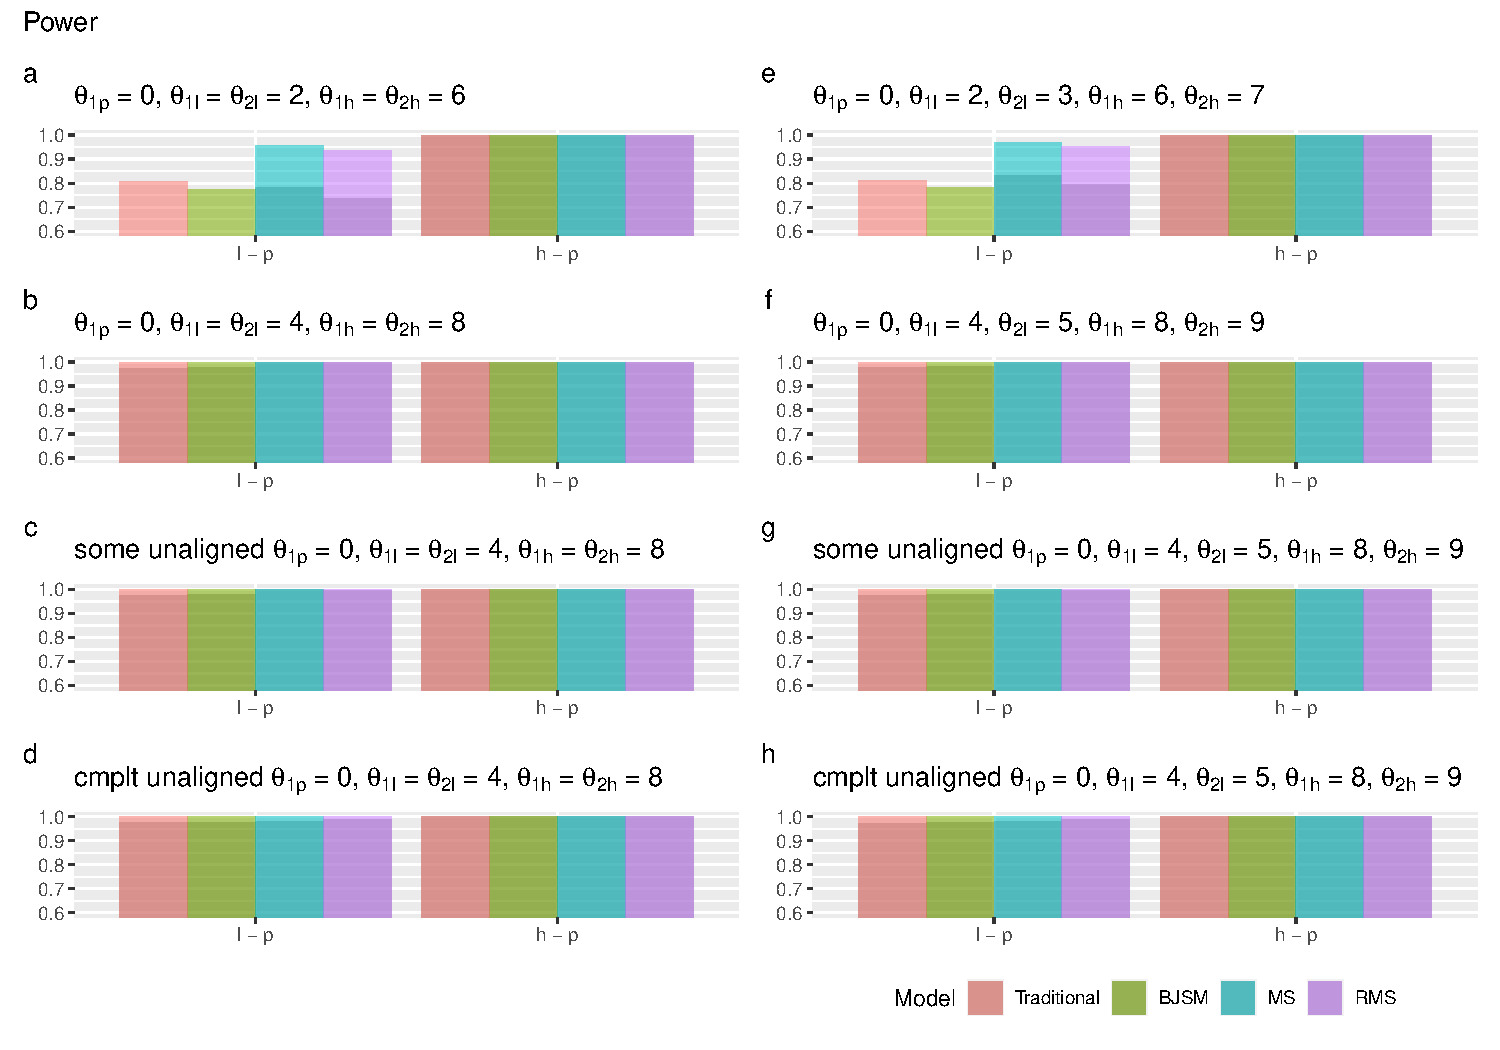
\includegraphics[width=16cm]{chapters/figures/CRpower.pdf}}
\caption{Simulated power of the MAC-snSMART methods}
\subcaption*{In this paper, the power is defined as the probability that the credible intervals of $\hat{\theta}_{1l} - \hat{\theta}_{1p}$ and $\hat{\theta}_{1h} - \hat{\theta}_{1p}$ do not include 0 when there are treatment effect difference between low dose and placebo and high dose and placebo. Two hierarchical models: MAC-snSMART (MS) and robust MAC-snSMART (RMS) are compared against the traditional method. The results of total sample size 50 are shown as the colored bars, while the results of total sample size 25 are shown as the overlaying grey bars. The simulation settings are described on the top of each graph. $\theta_{jk}$ denotes the true value of the expected treatment effects of treatment $k$ in stage $j$, where $j = 1, 2$, $k = P, L, H$, P = placebo, L = low dose, and H = high dose. \emph{external unaligned} means the placebo treatment effects in external control data are inconsistent with the placebo treatment effect in the current trial.}
\label{fig:Power}
\end{figure}

Our proposed robust MAC-snSMART method assumes fully exchangeable treatment effects across trial stages, and allows for differential heterogeneity and nonexchangeability in external control data. This method can be easily extended to include treatment effect nonexchangeability for low dose and high dose across trial stages.

The SPITFIRE trial and many other \ac{DMD} trials incorporate participant demographic and baseline characteristics covariates in their analysis. In the future, we hope to extend the \ac{snSMART} design and robust \ac{MAC}-snSMART method to include patient-level covariates and add an interim analysis at the end of stage 1, e.g., stopping for futility or dropping a treatment arm. In addition, data in \ac{DMD} trials is usually collected in a longitudinal manner with 3 or more visits. Future work can incorporate longitudinal data into our design and methods. 
% Place your additional chapters here using the \input{} command
\chapter{Dynamic Prediction of the Landmark Survival Time in Cancer Clinical Trials Using Joint Modeling Framework}
\label{chpt:chpt3}

\section{Introduction}
In recent years, many cancer drugs have received regulatory approvals based on \ac{PFS} as the primary endpoint. Although \ac{PFS} is a well-accepted surrogate endpoint for \ac{OS} in many cancer types, improvement in survival remains the clinical gold standard for assessing a patient's benefit \citep{tang2007surrogate, driscoll2009overall, methy2010surrogate, grigore2020surrogate}. However, planning a statistically well-powered \ac{OS} analysis in practice often presents challenges due to longer survival times in early-stage cancers, patients switching to alternative treatments after progression, starting other anti-cancer therapies, or being lost to follow-up. The timing of the primary analysis for trials with \ac{PFS} as the primary endpoint is determined by the number of patients progressed, and survival data is often not mature enough for meaningful statistical inference due to a low number of deaths. Hence, if \ac{PFS} is statistically significant in the final analysis, regulatory agencies often request one or more updated \ac{OS} analyses once the survival data are more mature. Updated \ac{OS} analyses are crucial for market access and reimbursement decisions. Therefore, proper planning is essential to ascertain when mature \ac{OS} data will be available.

Model-based prediction of survival time for trial participants aids research teams in efficiently allocating resources, accurately planning future \ac{OS} analyses, and understanding the potential survival benefit of an experimental drug. It also assists in designing and committing to Phase 3 trials based on disease progression data observed in Phase 2 studies. Moreover, it helps clinicians and scientists understand the mechanism of a new compound that improves patients' survival while reducing disease burden. Besides drug development, mature \ac{OS} data are crucial for decision-making by both patients and clinicians, and understanding a drug's cost-effectiveness. \cite{sborov2019impact} demonstrated that when oncologists inaccurately predict \ac{OS}, patients with advanced cancer are more likely to receive aggressive end-of-life care, often contradicting the patients' wishes. \cite{mackillop1997measuring} stated that accurate \ac{OS} prediction facilitates the effective use of limited healthcare resources and helps patients make suitable plans for their remaining lives. \cite{henderson2001accuracy} further provides examples of how accurate survival predictions have financial implications for insurance programs and health authorities.

\ac{PFS} is defined as the time from randomization until \ac{PD} or death from any cause. In oncology studies, progression is evaluated using the \ac{RECIST} \citep{eisenhauer2009new}. \ac{RECIST} provides standardized definitions and procedures for documenting how subjects progress, respond, or remain stable in terms of their disease burden during a treatment course. \ac{RECIST} offers methods for assessing solid tumor responses using X-ray, CT, and MRI scans and is recommended by the National Cancer Institute. Note, \ac{PFS} is viewed as a composite outcome with four components: 1) measurement of the target lesion, which is captured as longitudinal continuous data, 2) time to non-target lesion progression, 3) time until the emergence of a new lesion, and 4) time to death from any cause. Depending on the cancer type, each of these components has a different degree of predictivity for \ac{OS}. For example, \cite{stein2013survival} showed that the progression of non-target lesions or the appearance of new lesions is more predictive of \ac{OS} benefit than the sum of the longest tumor diameters of the target lesions for patients with metastatic renal cell carcinoma. The current practice of \ac{OS} prediction often overlooks the disease progression process and models only the number of deaths.

In this manuscript, we evaluated several model-based approaches to forecast the death times of trial participants ``still alive", leveraging information about disease progression along with important baseline factors. The relationship between \ac{PFS} and \ac{OS} has garnered interest in both statistical and clinical literature over time. Notably, \cite{fleischer2009statistical} employed exponential time-to-event distributions to describe the dependency structure between \ac{OS} and \ac{PFS}. This is further expanded by \cite{weber2019quantifying, fu2013joint, meller2019joint} by utilizing copula and multi-state models to jointly analyze \ac{PFS} and \ac{OS} without strict parametric assumptions for the marginal survival distributions of \ac{PFS} and \ac{OS}. Another important work by \cite{shukuya2016relationship} investigated the correlation between median \ac{PFS} and median \ac{OS}, concluding that both tumor response and \ac{PFS} are significant predictors of \ac{OS}. Other methodologies for \ac{OS} prediction include joint modeling of longitudinal tumor size data of the target tumor and survival data (\cite{claret2009model, claret2013evaluation, wang2009elucidation, bruno2014evaluation, zecchin2016models, lim2019predicting}), which incorporates baseline survival data into the \ac{OS} prediction. Meanwhile, \cite{yu2020new} jointly modeled the dynamics of target lesions and the progression of non-target lesions to predict \ac{PFS}. However, most of the literature in this area focuses primarily on improving the estimation of \ac{OS} rather than predicting the future survival time of patients ongoing in the trial. Moreover, to our current knowledge, there is no existing methodology that formally combines all three components of disease progression, i.e., target lesion, non-target lesion and new lesion. In this paper, we propose a joint modeling framework to address these gaps and further enhance the copula model and the multi-state model for predicting the survival times of ongoing patients.

The rest of the paper is structured as follows: A motivating example from a Phase 3 renal cell carcinoma study is used to establish the problem in Section \ref{sec:example}. This is followed by a set of proposed models that explore the correlation between disease progression and survival as presented in Section \ref{sec:method}. The simulation studies conducted to test the properties of our method are presented in Section \ref{sec:simulation}. The renal cell carcinoma example is revisited in Section \ref{sec:caseanalysis} to illustrate the practical utility of the proposed methodology. Finally, we conclude with a discussion that summarizes the key messages and lessons learned.

\section{Motivating Example: Phase 3 Study in Renal Cell Carcinoma} \label{sec:example}
The methods outlined in this paper are inspired by a phase 3, randomized, open-label, parallel-arm study. A total of 800 treatment-naive adult participants with advanced renal cell carcinoma were randomized (1:1) to receive either the experimental drug or the standard of care. A key inclusion criterion was the presence of at least one measurable lesion, as defined by \ac{RECIST} version 1.1, which had not been previously irradiated. Tumor assessments were performed using computed tomography or magnetic resonance imaging at baseline, every six weeks post-randomization for the first 18 months, and subsequently every 12 weeks until confirmed disease progression. Important baseline demographic and disease characteristics were evenly distributed between the two treatment groups. The study had two primary endpoints: \ac{PFS} and \ac{OS} among patients with programmed death ligand 1 (PD-L1)–positive tumors. The primary analysis was scheduled when at least 397 \ac{PFS} events occurred (Figure \ref{fig:evolution}). At the time of the primary \ac{PFS} analysis only 146 deaths were observed which was immature to draw any reasonable conclusion for OS. Therefore, an updated analysis of \ac{OS} was planned after 341 deaths. The trial findings indicated that patients administered the experimental drug experienced a notably extended \ac{PFS} compared to those given the standard of care. It is crucial to note that while we have utilized the data structure from a real-life trial, the actual values presented here are simulated based on published summary statistics, both for proprietary considerations and to ensure proper protection of patient data.

\begin{figure}
    \centering
    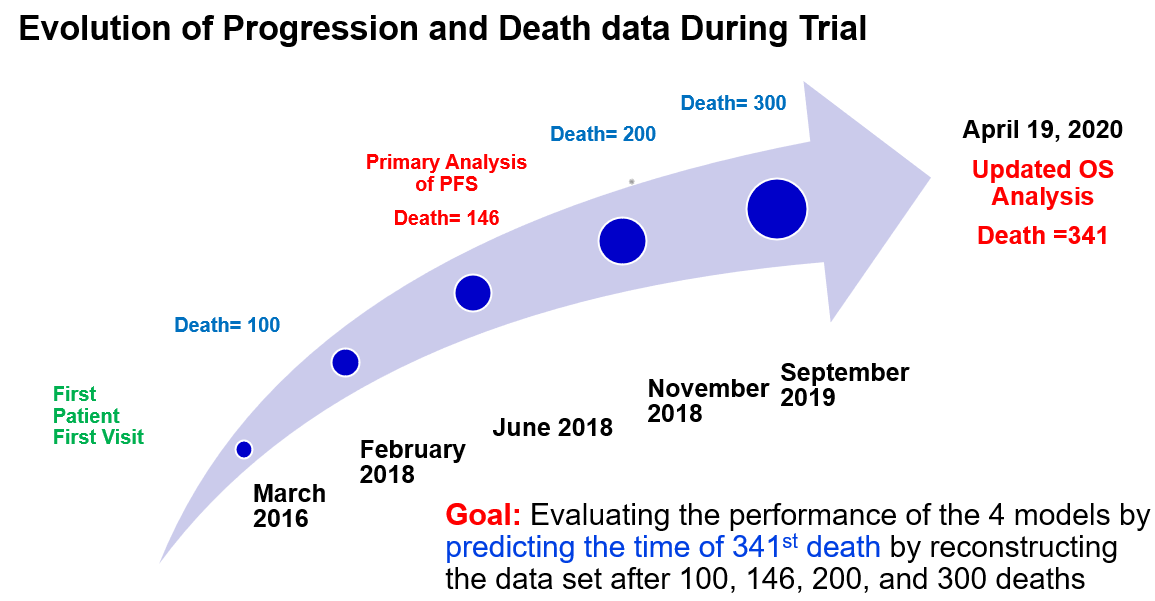
\includegraphics[width=0.85\textwidth]{chapters/figures/Evolution.png}
    \caption{Evolution of progression and death data during trial\label{fig:evolution}}
\end{figure}


We aim to use the observed data to construct a predictive tool that provides a reliable estimate of the time of the $n$th death in the trial. Specifically, we utilize data on participants' baseline characteristics, treatment group, \ac{OS}, and the processes underlying \ac{PFS}, including measurements of target lesions and the progression of disease in non-target and new lesions. This approach is justified as \ac{PFS} is known to be a strong predictor of \ac{OS} in advanced renal cell carcinoma \citep{heng2011progression}

Figure \ref{fig:profile_LD} demonstrates significant variability among individuals in the sum of the longest diameters of target lesions, making it difficult to draw any conclusions about the treatment without systematic modeling of this variability. Moreover, Kaplan-Meier plots for non-target lesions and new lesions are shown in Figures \ref{fig:NT_KMplot} and \ref{fig:NL_KMplot}, respectively. From both plots, we observe differences between the two treatment arms: patients who received the experimental drug exhibited a longer time to \ac{PD} when considering assessments of non-target lesions and new lesions. A similar trend is also observed in the Kaplan-Meier plots for \ac{OS} (Figure \ref{fig:OS_KMplot}) and \ac{PFS} (Figure \ref{fig:PFS_KMplot})

\begin{figure}
    \centering
    \subfloat[]{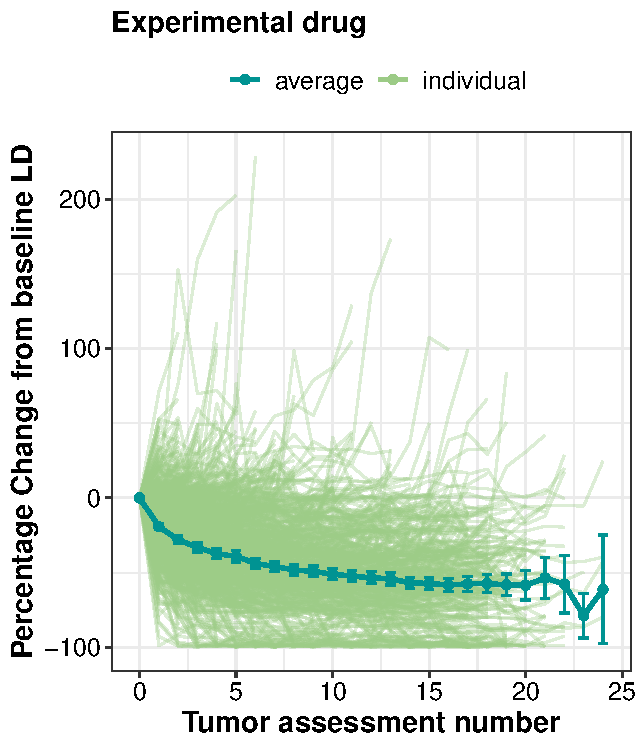
\includegraphics[width=0.45\textwidth]{chapters/figures/profile_LD_exp.pdf}\label{fig:profile_LD_exp}}
    \hfill
    \subfloat[]{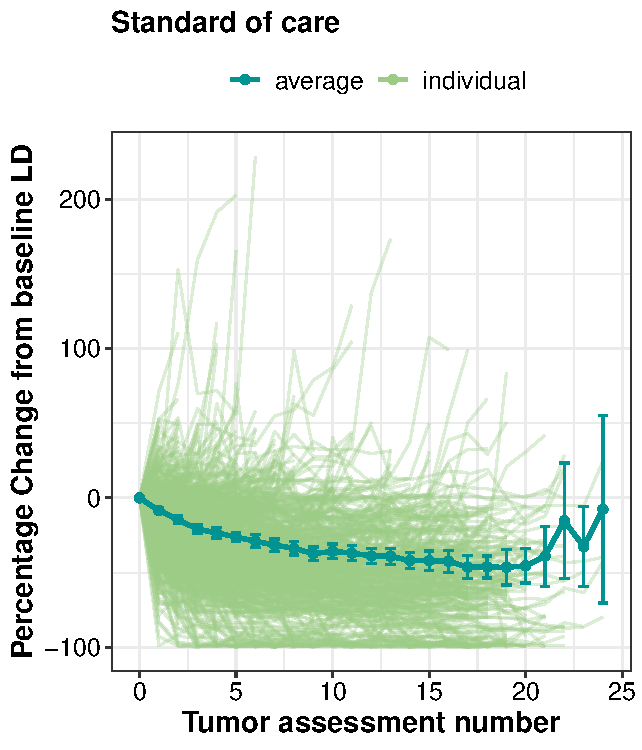
\includegraphics[width=0.45\textwidth]{chapters/figures/profile_LD_soc.pdf}\label{fig:profile_LD_soc}}
    \caption{Profile plot of the sum of the longest diameter of target lesions}
    \label{fig:profile_LD}
\end{figure}

\begin{figure}
    \centering
    \subfloat[]{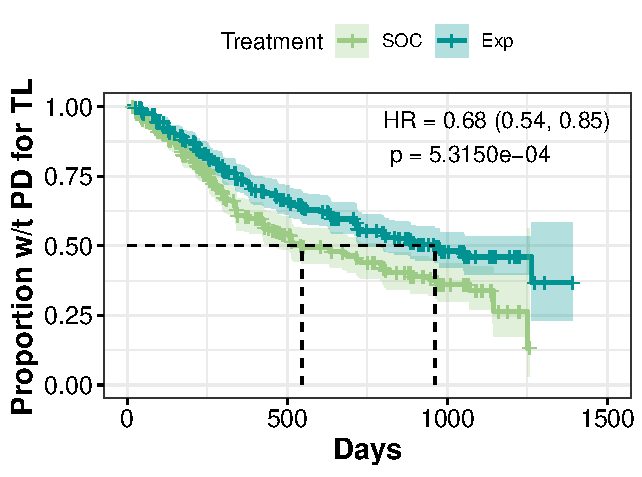
\includegraphics[width=0.45\textwidth]{chapters/figures/TL_KMplot.pdf}\label{fig:TL_KMplot}}
    \subfloat[]{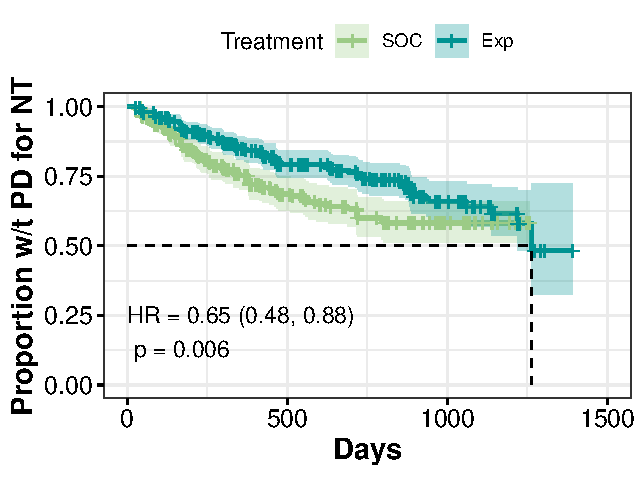
\includegraphics[width=0.45\textwidth]{chapters/figures/NT_KMplot.pdf}\label{fig:NT_KMplot}}
    \hfill
    \subfloat[]{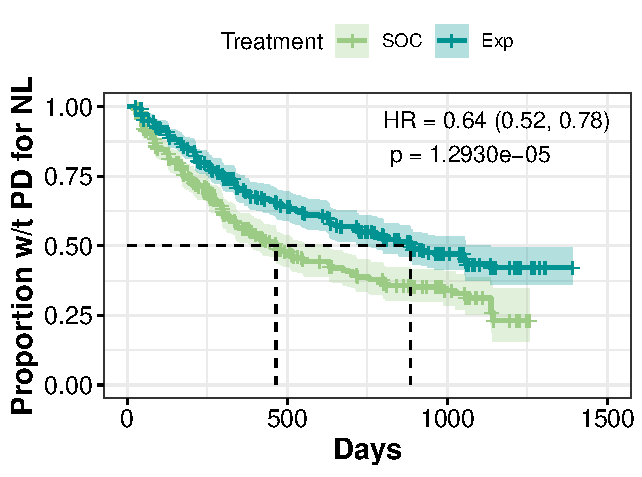
\includegraphics[width=0.45\textwidth]{chapters/figures/NL_KMplot.pdf}\label{fig:NL_KMplot}}
    \subfloat[]{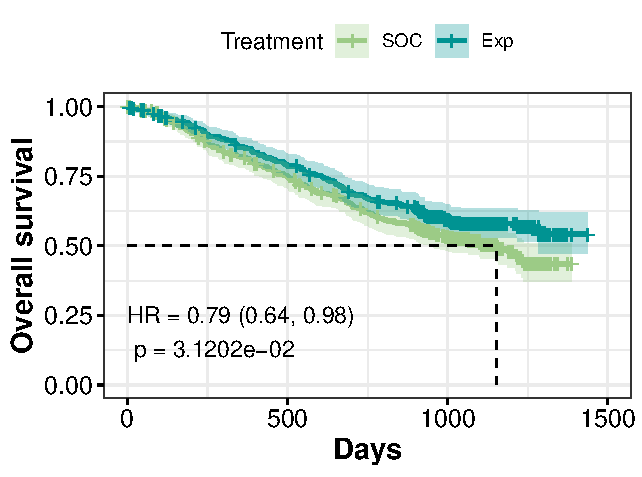
\includegraphics[width=0.45\textwidth]{chapters/figures/OS_KMplot.pdf}\label{fig:OS_KMplot}}
    \hfill
    \subfloat[]{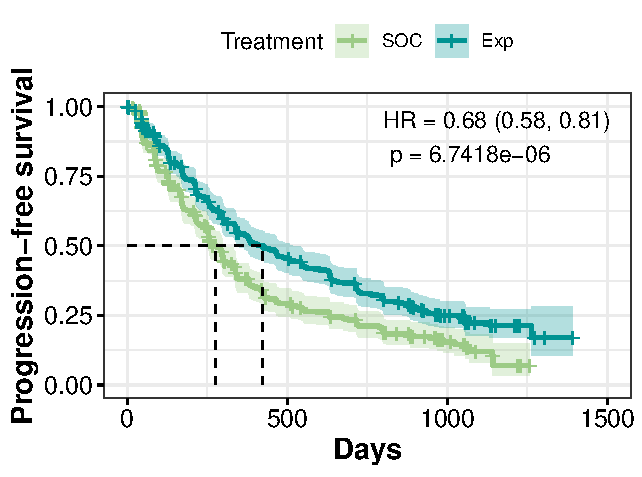
\includegraphics[width=0.45\textwidth]{chapters/figures/PFS_KMplot.pdf}\label{fig:PFS_KMplot}}
    \caption{Kaplan-Meier plots of time to progressive disease at the time of updated OS analysis considering target lesions (a), non-target lesions (b), new lesions (c), time to progressive design considering overall survival (d), and progression-free survival (e).}
\end{figure}


\section{Method}
\label{sec:method}
In this manuscript, the general process of using Bayesian statistical models to generate \ac{OS} predictions is as follows: At any given point during the clinical trial, we collect the current data and input it into our Bayesian models. Subsequently, a Markov chain Monte Carlo (MCMC) process is utilized to estimate the parameters. These estimations are then used to generate predicted \ac{OS} outcomes by leveraging the posterior predictive distribution (PPD) technique. This process allows us to create a predictive framework that is both dynamic and reflective of the evolving nature of trial data, providing timely and robust predictions for OS.


\subsection{Bayesian Model-Averaged Joint Modeling Approach}
\label{sec:jm}

In this section, we outline our proposed model by establishing three distinct joint models between each of the processes of disease progression and OS. These three joint models include the joint model between the sum of the longest diameter of target lesions and OS, the joint model between the time to non-target lesion \ac{PD} and OS, and the joint model between the time to new lesion \ac{PD} and OS. Furthermore, we incorporate a marginal model directly modeling OS. Three main steps are included in our model. First, we mitigate ``information loss" by considering all four granular components of PFS. By constructing joint, marginal models for each component, we derive real-time \ac{OS} predictions from each trial participants ``still alive". This results in four sets of intermediate predictions. Second, our proposed methods fully encapsulate the association between progression and death by incorporating random processes. Third, we enhance the accuracy of \ac{OS} predictions from \ac{PFS} by deriving the final \ac{OS} prediction from all four models' intermediate predictions simultaneously using \ac{BMA} \citep{hoeting1999bayesian}. Using the \ac{BMA} technique, we blend these different predictions to create a final predicted OS, which combines all four individual forecasts with appropriate weights. Thus, joint modeling represents a promising scientific approach to overcoming the challenges associated with \ac{OS} prediction, in comparison to existing methods that will be discussed in the subsequent sections. The structure of the proposed multivariate joint modeling approach is illustrated in Figure \ref{fig:JM}, with details provided in the following subsections.
\subsubsection{Joint Model for the Association between Target Lesion and OS} \label{sec:TL}


\begin{figure}
\centering
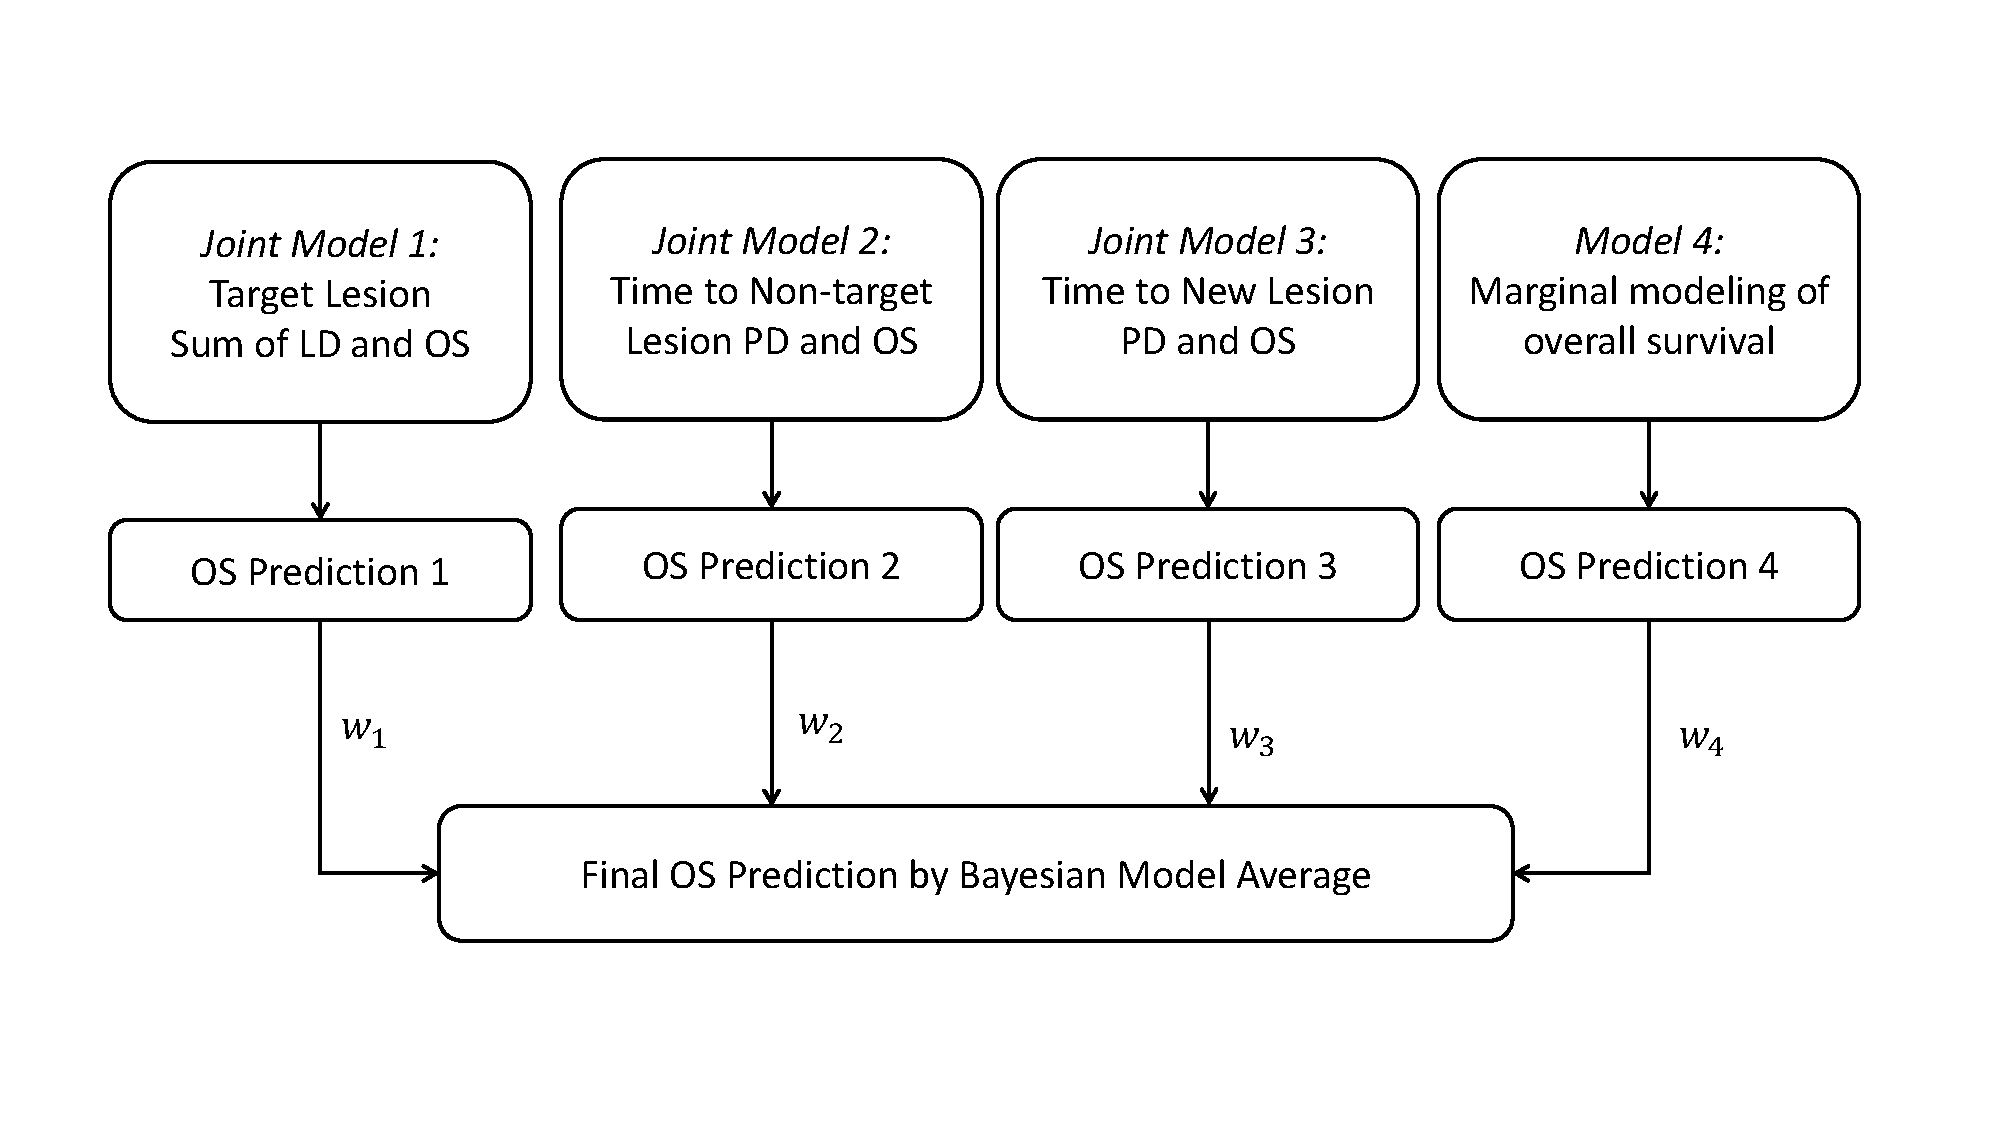
\includegraphics[width=\textwidth]{chapters/figures/JM.pdf}
%\\
%\subfloat[]{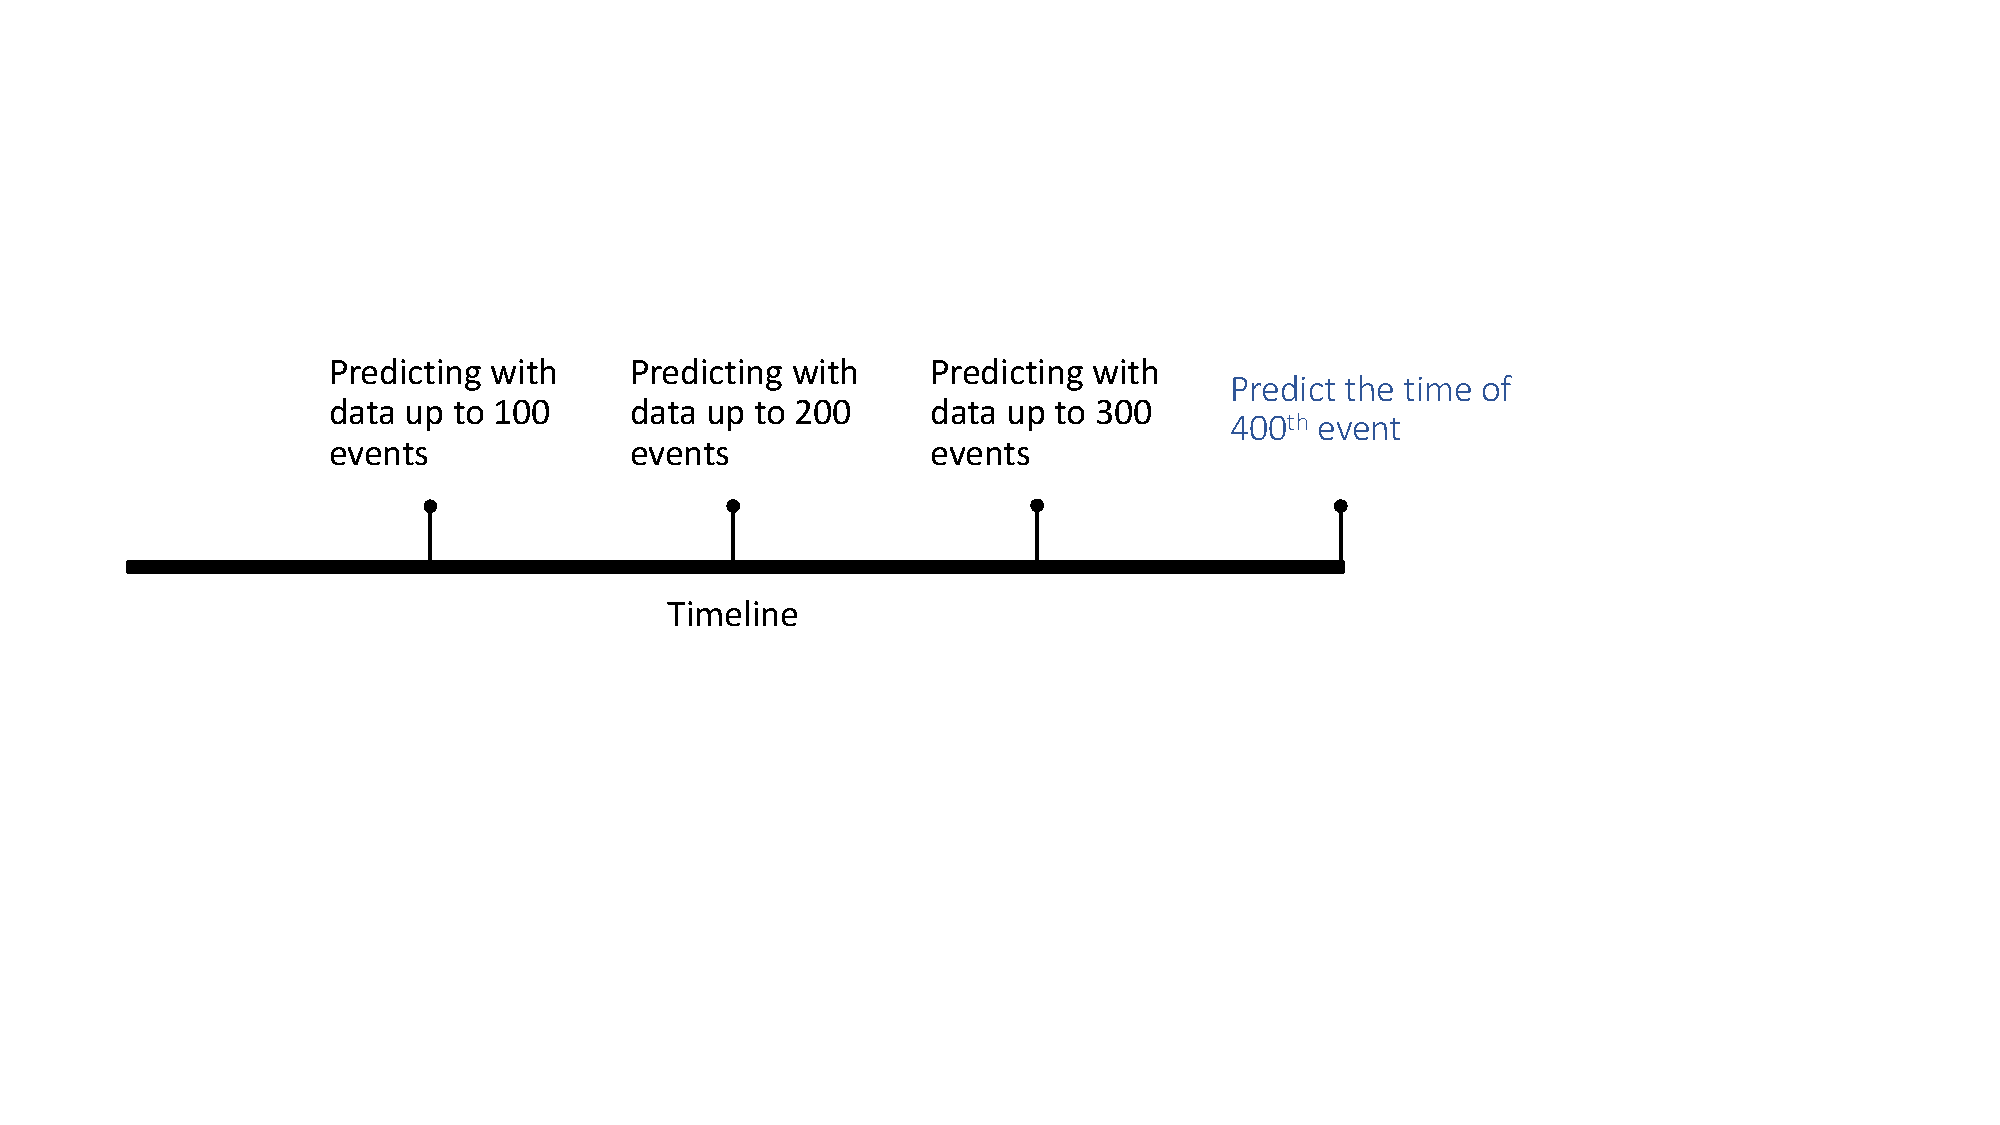
\includegraphics[width=\textwidth]{img/timeline.pdf}\label{fig:timeline}}
\caption{Multivariate joint modeling structure.} 
%(b) Predict the time of last (400th) event with observed data up to 100/200/300 events.}
\label{fig:JM}
\end{figure}


We consider a set of $n$ subjects followed over an interval of time [0,$\tau$]. Let $z_{ij}$ be the target lesion measurement (or \% change from baseline) at time $t_{ij}$ (for the $i$-th participant at the $j$-th visit), where $i=1,...,n$ and $j=1,...,k_i$. We assume the target lesion measurement time $t_{ij}$ is non-informative so that it is independent of the longitudinal measurement and event-time processes for OS. We define a latent zero-mean Gaussian process $W_i(t)$ for the $i$-th participant, independent of different participants. The following sub-models link the joint model of lesion measurements and OS:

The observed lesion measurement
$Y_{i}(t)=\mu_{i}(t)+\epsilon_i$,
where $\epsilon_i$ is the measurement error, and the lesion measurement process $\mu_{i1}$, $\mu_{i2}$,...
is modeled by the linear model
$\mu_{i}(t)=\textbf{X}_i(t)' \boldsymbol{\beta}_{\mu}+W_{i}(t)$. Here, $\textbf{X}_i(t)$ is the time-dependent covariate matrix for subject $i$'s lesion measurement. $W_i(t)$ is a Gaussian process that has the form $W_{1i}(t)=b_{1i}+b_{2i}t$,
where ($b_{1i},b_{2i}$) are zero-mean bivariate Gaussian variables with variances $\sigma_1^2$ and $\sigma_2^2$ respectively, and correlation coefficient $\rho$. 

The \ac{OS} process at time t is modeled by
$\lambda(t)=\lambda_0(t) \exp(\textbf{Z}_i' \boldsymbol{\beta}_{\rm OS}+\lambda \mu_{i}(t)+b_{3i})$.
Under a Weibull baseline hazard, $\lambda(t)$ has the form
$\lambda(t)=\alpha_{\rm OS,TL} \gamma_{\rm OS} t^{\alpha_{\rm OS,TL}-1} \exp(\textbf{Z}_i' \boldsymbol{\beta}_{\rm OS}+\lambda \mu_{i}(t)+b_{3i})$,
where $\textbf{Z}_i$ is the covariate matrix for OS, $\gamma_{\rm OS}$ and $\alpha_{\rm OS,TL}$ are the scale and shape parameters
of the Weibull distribution, and $b_{3i}\sim N(0,{\sigma_3})^2$ are random effects orthogonal to the measurement process. The construction of the likelihood for this joint model is detailed below:

The marginal distribution of the observed measurements $\mu$ is easily obtained. The likelihood for the observed data can be factorized as the product of this marginal distribution and the conditional distribution of OS, given the observed values of $\mu$. Let $\boldsymbol{\theta}_1$ denote the combined vector of unknown parameters. Conditional on lesion measurements $\mu$, OS is independent of these measurements $\mu$, so we can write the likelihood $L=L(\boldsymbol{\theta}_1, \mu, OS)$ as
$L=L_{\mu}(\boldsymbol{\theta}_1,\mu)  \times L_{OS| \mu}(\boldsymbol{\theta}_1,OS|\mu)
$,
where $L_{\mu}(\boldsymbol{\theta}_1,\mu)$ is of standard form corresponding to the marginal multivariate normal distribution of $\mu$ and
$$
L_{OS|\mu}(\boldsymbol{\theta}_1, OS|\mu)=\prod_i \bigg\{ \bigg[\lambda_0 (t) \exp(\textbf{Z}_i' \boldsymbol{\beta}_{\rm OS}+\lambda \mu_{i}(t)) \bigg]^{\delta_{OS,i}} 
$$
$$\times \exp \bigg[ -\int_0^{y_{OS,i}} \lambda_0(t) \exp(\textbf{Z}_i' \boldsymbol{\beta}_{\rm OS}+\lambda \mu_{i}(t))dt\bigg]\bigg\},
$$
here, $y_{OS,i}=\min(t_{OS,i},c_{OS,i})$ and $\delta_{OS,i}=I(t_{OS,i}\leq c_{OS,i})$. $c_{OS,i}$ is the censoring time for the $i$th participant and $t_{OS,i}$ is the true event time.


\subsubsection{Joint Model for the Association between Time to Non-Target Lesion and OS} \label{sec:NT}
Copulas are commonly used for modeling the dependence between random variables. They are continuous multivariate cumulative distributions with each random variable following a uniform marginal distribution on the interval $[0, 1]$.
Sklar's theorem states that any multivariate joint distribution can be written using univariate marginal distribution functions and a copula describing the variables' dependence structure \citep{sklar1959fonctions}. Therefore, copulas can be used to model the dependence between these survival times, allowing for more accurate prognostic prediction.
Here, we can use the copula to jointly model time to non-target lesion and OS, where time to non-target lesion corresponds to the time between randomization and \ac{PD} is observed under non-target lesion. A bivariate copula function $C:[0, 1]^2 \rightarrow [0, 1]$ of the endpoints (T, O), where $T:=$ \textit{time to non-target lesion} and $O:= OS$, can be expressed by joint survival function $\boldsymbol{S}(t, o) = T(T \geq t, O \geq o) = C(\boldsymbol{S}_{T}(t), \boldsymbol{S}_{O}(o)),$
where  $t,o \geq 0$, $\boldsymbol{S}_T$ and $\boldsymbol{S}_O$ are the marginal survival functions of $T$ and $O$, respectively \citep{weber2020statistical}. To capture various dependency patterns, one can employ different copula families. Here, we opt for the Clayton copula function \citep{clayton1978model}, which belongs to the Archimedean copula class and can capture strong dependence in the left tail. By doing so, we can express the relationship between time to non-target lesion and \ac{OS} using a single parameter $\eta_{NT}$, a parameter that can be directly linked to Kendall's tau, effectively characterizing their dependence. In the subsequent paragraphs, we formally define the copula model between time to non-target lesion and OS.

Let $t_{NT}$ and $t_{OS}$ denote times to non-target lesion and death (OS), respectively, and let $\textbf{Z}$ be covariates of interest.
For a participant with covariates $\textbf{Z}$, let $\lambda_{\rm NT}(t|\textbf{Z})$
denote the hazard function for the time to non-target lesion. Under the Cox
proportional hazards model, we have $\lambda_{\rm NT}(t_{NT}|\textbf{Z})=\lambda_{0, \rm NT}(t_{NT})\mathrm{exp}(\textbf{Z}' \boldsymbol{\beta_{\rm NT}})$.
When the baseline hazard $\lambda_{0, \rm NT}(t_{NT})$ is modeled by a Weibull
distribution, the corresponding survival function is given by
$S_{\rm NT}(t_{NT}|\textbf{Z})=\mathrm{exp}\{-\gamma_{\rm NT} t_{NT}^{\alpha_{\rm NT}}
\mathrm{exp}(\textbf{Z}' \boldsymbol{\beta_{\rm NT}} )\}$, such that $\gamma_{\rm NT}$ and $\alpha_{\rm NT}$ are the scale and shape parameters
of the Weibull distribution, respectively. Similarly, for \ac{OS} we have $S_{\rm OS}(t_{OS}|\textbf{Z})=\mathrm{exp}\{-\gamma_{\rm OS} t_{OS}^{\alpha_{\rm OSNT}}
\mathrm{exp}(\textbf{Z}' \boldsymbol{\beta_{\rm OSNT}} )\}$. Hence, the Clayton copula model can be specified as $S_1(t_{\rm NT},
t_{\rm OS}|\textbf{Z})=\{S_{\rm NT}(t_{\rm NT}|\textbf{Z})^{-\eta_{\rm NT}}
+S_{\rm OS}(t_{\rm OS}|\textbf{Z})^{-\eta_{\rm NT}}-1\}^{-1/\eta_{\rm NT}}$, 
where $\eta_{\rm NT}>0$ measures the correlation between time to non-target lesion and OS. To take into account the heterogeneity of the patient population, we introduce random effects for the shape parameter of the Weibull model denoted as $b_{NT_i}$ and $b_{OS_i}$. Therefore, we have $\alpha_{NT_i}=\alpha_{NT} + b_{NT_i}$, $\alpha_{OS_i}=\alpha_{OS}+b_{OS_i}$. The relationship between Kendall's $\tau$ and the correlation parameter $\eta_{\rm NT}$
is $\tau_{\rm NT} = \eta_{\rm NT}/(2+\eta_{\rm NT})$. A large value of $\eta_{\rm NT}$
represents a high correlation. When $\eta$ goes to 0,
the correlation approaches 0, and when $\eta_{\rm NT}$ goes to $\infty$, the correlation converges to 1. 
For non-target lesion, we define $y_{\rm NT}=\mathrm{min}(t_{\rm NT}, c_{\rm NT})$ and
$\delta_{\rm NT}=I(t_{\rm NT} \le c_{\rm NT})$,
where $c_{\rm NT}$ and $I(\cdot)$ denote the censoring time and the indicator function,
respectively; and define $y_{\rm OS}$ and $\delta_{\rm OS}$ similarly for OS.

Depending on the censoring pattern, the observed data for the $i$th participant falls into one of the following mutually exclusive cases: 1) both $t_{NT}$ and $t_{OS}$ are observed ($\delta_{NT}$=1, $\delta_{OS}$=1), 2) $t_{NT}$ is observed and $t_{OS}$ is censored ($\delta_{NT}$=1, $\delta_{OS}$=0), 3) $t_{NT}$ is censored and $t_{OS}$ is observed ($\delta_{NT}$=0, $\delta_{OS}$=1), and 4) both $t_{NT}$ and $t_{OS}$ are censored ($\delta_{NT}$=0, $\delta_{OS}$=0). Based on these four scenarios, we can derive the likelihood of the copula model with the following steps:

Let
$\boldsymbol{\theta}_2=(\boldsymbol{\beta_{\rm NT}}, \alpha_{\rm NT}, \lambda_{\rm NT}, \boldsymbol{\beta_{\rm OSNT}},
\alpha_{\rm OSNT}, \lambda_{\rm OS}, \eta_{\rm NT})$,  then the
likelihood for the $i$th patient with ${\rm Data}_i=(y_{\rm NT}, y_{\rm OS},
\delta_{\rm NT}, \delta_{\rm OS}, \textbf{Z})_i$ is given by
$$
L(\boldsymbol{\theta}_2|{\rm Data}_i)
=L_1^{\delta_{\rm NT}\delta_{\rm OS}}
L_2^{\delta_{\rm NT}(1-\delta_{\rm OS})}L_3^{(1-\delta_{\rm NT})\delta_{\rm OS}}
L_4^{(1-\delta_{\rm NT})(1-\delta_{\rm OS})}, 
$$

where

\begin{align*}
L_1 &=\frac{\partial^2\, S_1(t_{\rm NT}, t_{\rm OS}|\textbf{Z})}{\partial t_{\rm NT} \partial t_{\rm OS}}\big|_{t_{\rm NT}=y_{\rm NT},t_{\rm OS}=y_{\rm OS}}
\\
& =\bigg(\eta_{\rm NT}+1\bigg)\bigg(\mathrm{exp}\{-\gamma_{\rm NT} y_{\rm NT}^{\alpha_{\rm NT}}
\mathrm{exp}(\textbf{Z}' \boldsymbol{\beta_{\rm NT}} )\} \mathrm{exp}\{-\gamma_{\rm OS} y_{\rm OS}^{\alpha_{\rm OSNT}}
\mathrm{exp}(\textbf{Z}' \boldsymbol{\beta_{\rm OSNT}} )\}\bigg)^{-(\eta_{\rm NT}+1)} \\
& \times \bigg(\mathrm{exp}\{-\gamma_{\rm NT} y_{\rm NT}^{\alpha_{\rm NT}}
\mathrm{exp}(\textbf{Z}' \boldsymbol{\beta_{\rm NT}} )\}^{-\eta_{\rm NT}}+\mathrm{exp}\{-\gamma_{\rm OS} y_{\rm OS}^{\alpha_{\rm OSNT}}
\mathrm{exp}(\textbf{Z}' \boldsymbol{\beta_{\rm OSNT}} )\}^{-\eta_{\rm NT}}-1\bigg)^{-\frac{2\eta_{\rm NT}+1}{\eta_{\rm NT}}} \\
&\times \gamma_{\rm NT} \alpha_{\rm NT} y_{\rm NT}^{{\alpha_{\rm NT} -1}} \exp(\textbf{Z}' \boldsymbol{\beta_{\rm NT}}) \mathrm{exp}\{-\gamma_{\rm NT} t^{\alpha_{\rm NT}}
\mathrm{exp}(\textbf{Z}' \boldsymbol{\beta_{\rm NT}} )\}\\
&\times \gamma_{\rm OS} \alpha_{\rm OSNT} y_{\rm OS}^{{\alpha_{\rm OSNT} -1}} \exp(\textbf{Z}' \boldsymbol{\beta_{\rm OSNT}}) \mathrm{exp}\{-\gamma_{\rm OS} t^{\alpha_{\rm OSNT}}
\mathrm{exp}(\textbf{Z}' \boldsymbol{\beta_{\rm OSNT}} )\},
\end{align*}

and


\begin{align*}
L_2&=-\frac{\partial S_1(t_{\rm NT}, t_{\rm OS}|\textbf{Z})}{\partial t_{\rm NT}}\bigg|_{t_{\rm NT}=y_{\rm NT},t_{\rm OS}=y_{\rm OS}} \\
&=-\bigg(\mathrm{exp}\{-\gamma_{\rm NT} y_{\rm NT}^{\alpha_{\rm NT}}
\mathrm{exp}(\textbf{Z}' \boldsymbol{\beta_{\rm NT}} )\}\bigg)^{-(\eta_{\rm NT}+1)}\\
&\times \bigg(\mathrm{exp}\{-\gamma_{\rm NT} y_{\rm NT}^{\alpha_{\rm NT}}
\mathrm{exp}(\textbf{Z}' \boldsymbol{\beta_{\rm NT}} )\}^{-\eta_{\rm NT}}+\mathrm{exp}\{-\gamma_{\rm OS} y_{\rm OS}^{\alpha_{\rm OSNT}}
\mathrm{exp}(\textbf{Z}' \boldsymbol{\beta_{\rm OSNT}} )\}^{-\eta_{\rm NT}}-1\bigg)^{-\frac{\eta_{\rm NT}+1}{\eta_{\rm NT}}}\\
&\times \gamma_{\rm NT} \alpha_{\rm NT} y_{\rm NT}^{{\alpha_{\rm NT} -1}} \exp(\textbf{Z}' \boldsymbol{\beta_{\rm NT}}) \mathrm{exp}\{-\gamma_{\rm NT} t^{\alpha_{\rm NT}}
\mathrm{exp}(\textbf{Z}' \boldsymbol{\beta_{\rm NT}} )\},
\end{align*}


and


\begin{align*}
L_3&=-\frac{\partial S_1(t_{\rm NT}, t_{\rm OS}|\textbf{Z})}{\partial t_{\rm OS}}\bigg|_{t_{\rm NT}=y_{\rm NT},t_{\rm OS}=y_{\rm OS}}\\
&=-\bigg(\mathrm{exp}\{-\gamma_{\rm OS} y_{\rm OS}^{\alpha_{\rm OSNT}}
\mathrm{exp}(\textbf{Z}' \boldsymbol{\beta_{\rm OSNT}} )\}\bigg)^{-(\eta_{\rm NT}+1)}\\
&\times \bigg(\mathrm{exp}\{-\gamma_{\rm NT} y_{\rm NT}^{\alpha_{\rm NT}}
\mathrm{exp}(\textbf{Z}' \boldsymbol{\beta_{\rm NT}} )\}^{-\eta_{\rm NT}}+\mathrm{exp}\{-\gamma_{\rm OS} y_{\rm OS}^{\alpha_{\rm OSNT}}
\mathrm{exp}(\textbf{Z}' \boldsymbol{\beta_{\rm OSNT}} )\}^{-\eta_{\rm NT}}-1\bigg)^{-\frac{\eta_{\rm NT}+1}{\eta_{\rm NT}}}\\
&\times \gamma_{\rm OS} \alpha_{\rm OSNT} y_{\rm OS}^{{\alpha_{\rm OSNT} -1}} \exp(\textbf{Z}' \boldsymbol{\beta_{\rm OSNT}}) \mathrm{exp}\{-\gamma_{\rm OS} t^{\alpha_{\rm OSNT}}
\mathrm{exp}(\textbf{Z}' \boldsymbol{\beta_{\rm OSNT}} )\},
\end{align*}


and

\begin{align*}
L_4&=S_1(t_{\rm NT}, t_{\rm OS}|\textbf{Z})\bigg|_{t_{\rm NT}=y_{\rm NT},t_{\rm OS}=y_{\rm OS}}\\
&=\{\mathrm{exp}\{-\gamma_{\rm NT} y_{\rm NT}^{\alpha_{\rm NT}}
\mathrm{exp}(\textbf{Z}' \boldsymbol{\beta_{\rm NT}} )\}^{-\eta_{\rm NT}}
+\mathrm{exp}\{-\gamma_{\rm OS} y_{\rm OS}^{\alpha_{\rm OSNT}}
\mathrm{exp}(\textbf{Z}' \boldsymbol{\beta_{\rm OSNT}} )\}^{-\eta_{\rm NT}}-1\}^{-1/\eta_{\rm NT}}.
\end{align*}

For a given subject, L1, L2, L3 and L4 correspond to the likelihood components that both NT and OS are observed, NT is observed but OS is censored, NT is censored but OS is observed, and both NT and OS are censored, respectively.



\subsubsection{Joint Model for Time to New Lesion and OS} \label{sec:NL}
Similar to Section \ref{sec:NT}, for the relationship between time to new lesion and OS, we model
the bivariate time-to-event data using the \cite{clayton1978model} model,
$S_2(t_{\rm NL},
t_{\rm OS}|\textbf{Z})=\{S_{\rm NL}(t_{\rm NL}|\textbf{Z})^{-\eta_{\rm NL}}
+S_{\rm OS}(t_{\rm OS}|\textbf{Z})^{-\eta_{\rm NL}}-1\}^{-1/\eta_{\rm NL}}$. The derivation of this copula model's likelihood is similar to that specified in section \ref{sec:NT}.

\subsubsection{Marginal Model for OS} \label{sec:marginal}
As a standard way of modeling time to event data, we model \ac{OS} with a simple Weibull baseline hazard model that has the form
$\lambda(t)=\alpha_{\rm OS,M} \gamma_{\rm OS} t^{\alpha_{\rm OS,M}-1} \exp(\textbf{Z}_i' \boldsymbol{\beta_{M}})$,
where $\textbf{Z}_i$ is the covariate matrix for modeling OS.

\subsection{Semi-Markov Three-State Illness-Death Model}
\label{sec:multi-state}
At the time this paper is written, no literature has covered survival time prediction based on a multi-state model; here, we fill this gap in this section. A multi-state model is another common approach for modeling the event history of participants in clinical trials \citep{andersen2002multi, meira2009multi, putter2007tutorial}. Among the various multi-state models, the one that finds the widest application is the three-state illness-death model, which includes a singular immediate state denoting ``illness" (Figure \ref{fig:multistate}). In this paper, we employ the homogeneous semi-Markov assumption \citep{cox1977theory} for the illness-death model, which implies that the hazard of death after progression depends on time since progression rather than time since randomization. Therefore, for every patient, we examine two distinct periods: the time between randomization and progression, and the duration from progression to death. Both of these intervals are treated as separate components and modeled individually. A third scenario occurs when a patient passes away without experiencing progression. In the following paragraphs, we explain the specific mathematical details of the illness-death model.

\begin{figure}[H]
    \centering
    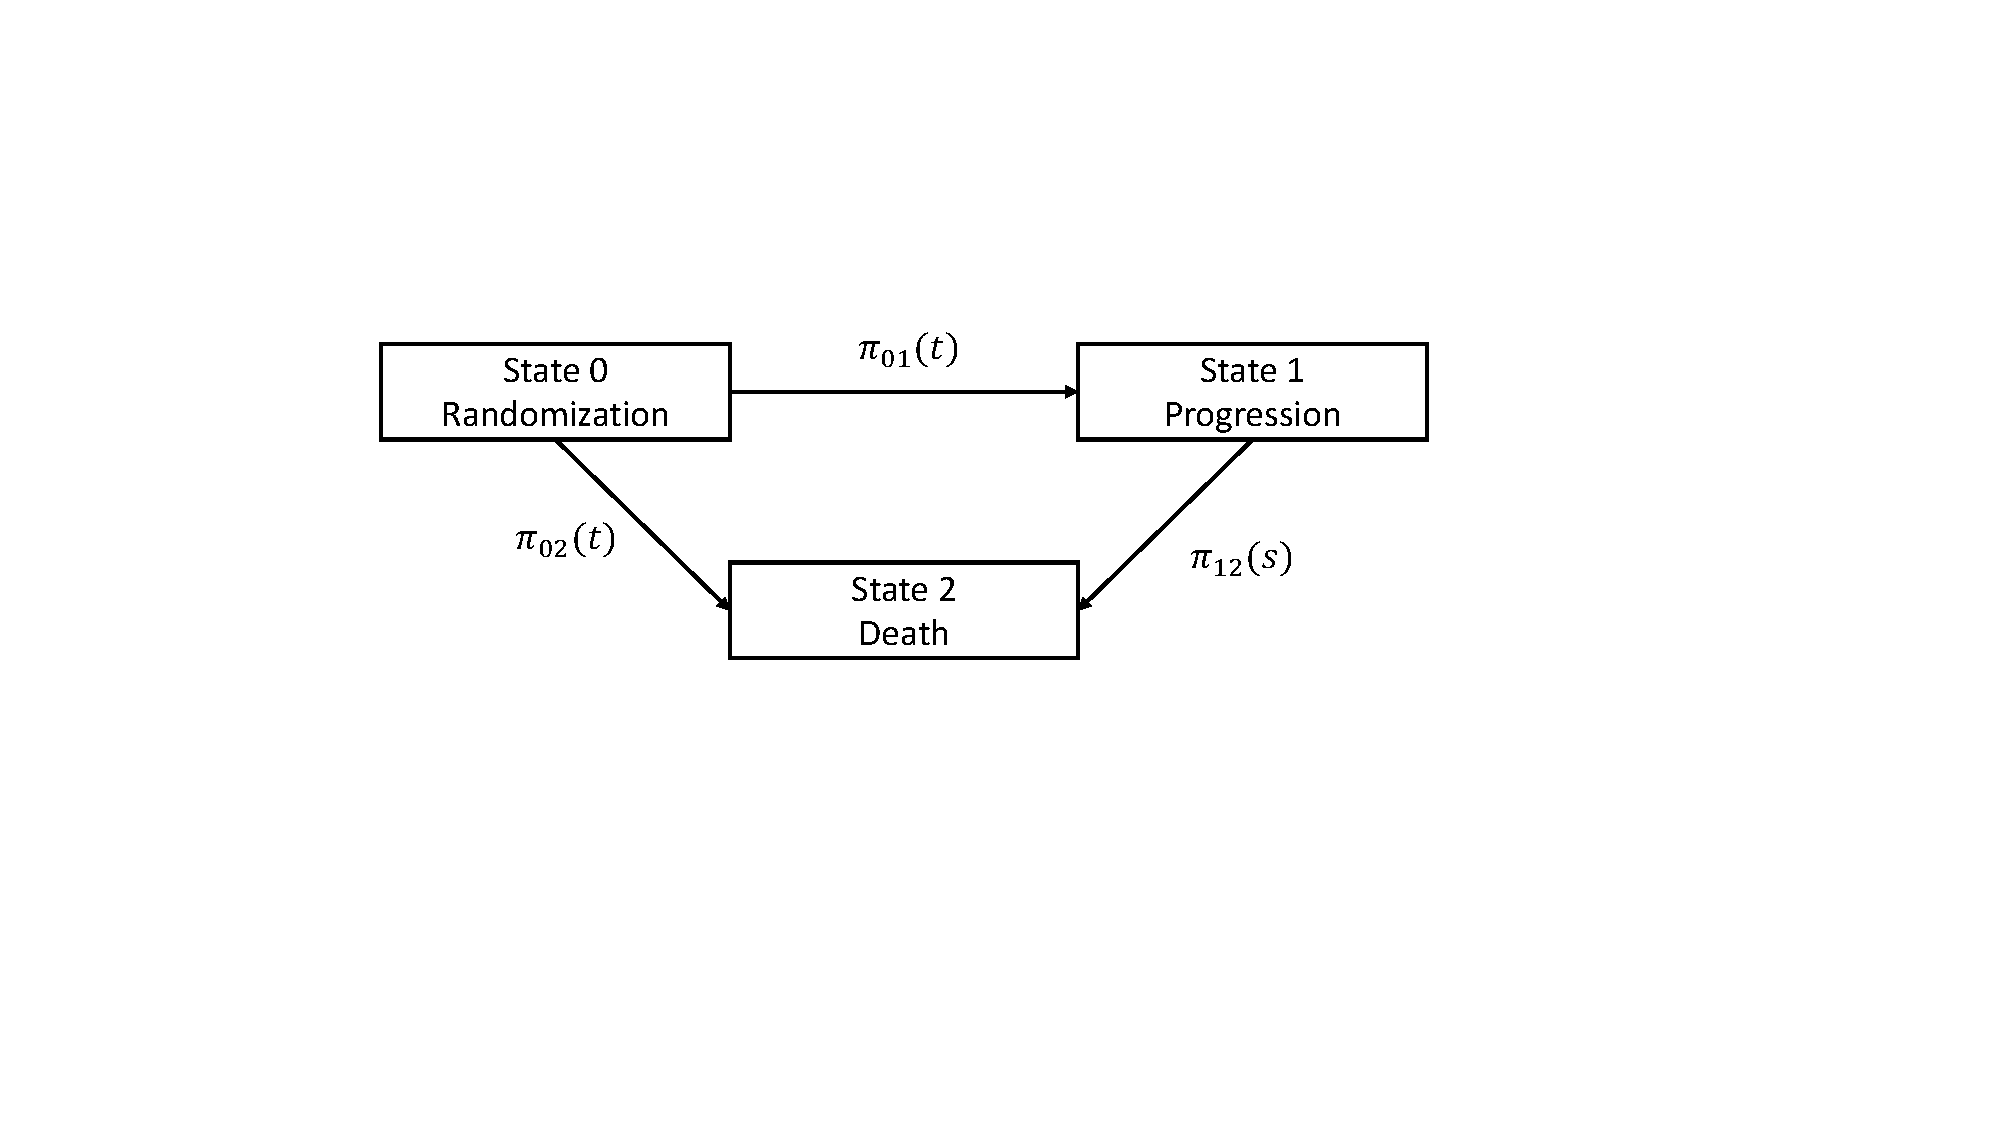
\includegraphics[width=0.7\textwidth]{chapters/figures/multi-state.pdf}
    \caption{The three-state illness-death model \label{fig:multistate}}
\end{figure}

For the illness-death model, transition probabilities represent the probabilities of transition from one state to another over a given time period. Here, we denote the transition probability as $P_{kl}(t_1, t_2)$ from time $t_1$ to $t_2$, where $k$, $l$ describes the state with $k \in {0, 1, 2}$ and $l \in {0, 1, 2}$. The expression of the transition probabilities are given by \citep{meira2009multi}:
$$P_{00}(t_1, t_2) = S_0(t_2 - t_1) = exp{(-\prod_{01}(t_2 - t_1) - \prod_{02}(t_2 - t_1))},$$
$$P_{11}(t_1, t_2) = S_1(t_2 - t_1) = exp{(-\prod_{12}(t_2 - t_1))},$$
$$P_{12}(t_1, t_2) = S_1(t_2 - t_1) = \int_{t_1}^{t_2}P_{11}(t_1, u) \pi_{12}(u;\mathcal{F}_u)P_{22}(u, t_2)du,$$
where $\prod_{kl}(t_1, t_2)=\int_{t_1}^{t_2}\pi_{kl}(t, \mathcal{F}_t)dt$ is the cumulative transition intensity between states $k$ and $l$, where $k \leq l$. If we consider the transition intensities $\pi_{kl}(t; \mathcal{F}_t)$ to follow Weibull distributions, they can be expressed as
$\pi_{01}(t)=\alpha\left(\frac{1}{\gamma_{01}}\right)^\alpha t^{\alpha - 1},$
$\pi_{02}(t)=\alpha\left(\frac{1}{\gamma_{02}}\right)^\alpha t^{\alpha - 1},$
and $\pi_{12}(s)=\alpha\left(\frac{1}{\gamma_{12}}\right)^\alpha s^{\alpha - 1},$
where $\gamma_{01}, \gamma_{02}$ and $\gamma_{03}$ are the scale parameters, $\alpha$ is the shape parameter, $t$ refers to time since randomization and $s$ refers to time since progression. $\gamma_{01}, \gamma_{02}$ and $\gamma_{03}$ for each patient are further defined as $\gamma_{01,i} = \Tilde{\gamma}_{01}exp(\boldsymbol{\beta}_{01}\boldsymbol{X}_i)$, $\gamma_{02,i} = \Tilde{\gamma}_{02}exp(\boldsymbol{\beta}_{02}\boldsymbol{X}_i)$, and $\gamma_{12,i} = \Tilde{\gamma}_{12}exp(\boldsymbol{\beta}_{12}\boldsymbol{X}_i)$, respectively, where $i \in N$, $\boldsymbol{X}_i$ is the vector of covariates, and $\boldsymbol{\beta}_{01}$, $\boldsymbol{\beta}_{02}$ and $\boldsymbol{\beta}_{12}$ are the regression coefficients. The baseline hazards $\Tilde{\gamma}_{01}$, $\Tilde{\gamma}_{02}$, and $\Tilde{\gamma}_{12}$ are estimated using a Weibull distribution. To guarantee the convergence of \ac{MCMC} , a uniform shape parameter $\alpha$ is employed for all three Weibull functions. The multi-state model's likelihood construction is as follows:

Here, we aim to estimate the parameter vector $\theta = (\alpha, \gamma_{01}, \gamma_{02}, \gamma_{12})$ using maximum likelihood estimation. Firstly, we need to model the survival experiences of individuals, which can be characterized by four distinct cases based on a patient's progression through the illness-death model:
1) Patients progress and are then censored,
2) Patients progress and subsequently die,
3) Patients die without prior progression,
4) Patients are censored without experiencing either progression or death. If for every individual \( i \) in the set \( (1, ..., n) \), we let \( t_{i1} \) indicate the duration from the initial state to either progression or death and let \( t_{i2} \), which is conditioned on progression, represents the time from progression to death, then the individual likelihood for these 4 experiences, denoted as \( L_i^{(k)}(\theta) \) where \( k \) varies from 1 to 4, can be described as: $L_i^{(1)}(\theta) = f_1(t_{i1})S_2(t_{i1})S_3(t_{i2})$, $L_i^{(2)}(\theta) = f_1(t_{i1})S_2(t_{i1})f_3(t_{i2})$, $L_i^{(3)}(\theta) = S_1(t_{i1})f_2(t_{i1})$, and $L_i^{(4)}(\theta) = S_1(t_{i1})S_2(t_{i1})$. Here, \( f_1(\cdot) \) and \( S_1(\cdot) \) are density and survival function for time to progression, \( f_2(\cdot) \) and \( S_2(\cdot) \) are density and survival function for time to death without progression, and \( f_3(\cdot) \) and \( S_3(\cdot) \) are density and survival function for time to death post progression. Therefore, comprehensive log-likelihood for all subjects can be formulated as:
\[
\begin{aligned}
\log(L(\theta)) &= \sum_{i=1}^{n}[(d_1)(1-d_2)(1-d_3)L_i^{(1)}(\theta) + (d_1)(1-d_2)(d_3)L_i^{(2)}(\theta) \\
&\quad +(1-d_1)(d_2)L_i^{(3)}(\theta) + (1-d_1)(1-d_2)L_i^{(4)}(\theta)],
\end{aligned}
\]

where \( d_1 \) is the censoring indicator for progression, \( d_2 \) is the indicator for death without preceding progression, and \( d_3 \) is the indicator for death post progression. Note: here, an indicator value of 0 represents censoring, whereas a value of 1 indicates the event's occurrence.


\subsection{Copula Model for Time-to-Progression (TTP) and OS} \label{sec:method_copula}
Similar to the model defined in  \ref{sec:NT}, we use $\lambda_{\rm TTP}(t|\textbf{Z})$ to
denote the hazard function for TTP. Under the Cox
proportional hazards model, we have $\lambda_{\rm TTP}(t|\textbf{Z})=\lambda_{0, \rm TTP}(t)\mathrm{exp}(\textbf{Z}' \boldsymbol{\beta_{\rm TTP}})$, and the corresponding survival function is given by
$S_{\rm TTP}(t|\textbf{Z})=\mathrm{exp}\{-\gamma_{\rm TTP} t^{\alpha_{\rm TTP}}
\mathrm{exp}(\textbf{Z}' \boldsymbol{\beta_{\rm TTP}} )\}$, such that $\gamma_{\rm TTP}$ and $\alpha_{\rm TTP}$ are the scale and shape parameters
of the Weibull distribution, respectively. The Clayton model between \ac{TTP} and \ac{OS} is specified as
\begin{equation*}
S_1(t_{\rm TTP},
t_{\rm OS}|\textbf{Z})=\{S_{\rm TTP}(t_{\rm TTP}|\textbf{Z})^{-\eta_{\rm TTP}}
+S_{\rm OS}(t_{\rm OS}|\textbf{Z})^{-\eta_{\rm TTP}}-1\}^{-1/\eta_{\rm TTP}}, 
\end{equation*}
where $\eta_{\rm TTP}>0$ measures the correlation.
For TTP,
define $y_{\rm TTP}=\mathrm{min}(t_{\rm TTP}, c_{\rm TTP})$ and
$\delta_{\rm TTP}=I(t_{\rm TTP} \le c_{\rm TTP})$,
where $c_{\rm TTP}$ and $I(\cdot)$ denote the censoring time and the indicator function,
respectively; and define $y_{\rm OS}$ and $\delta_{\rm OS}$ similarly for OS. Depending on the censoring pattern, the observed data for the $i$th participant falls into one of the 4 mutually exclusive cases: ($\delta_{TTP}$=1, $\delta_{OS}$=1), ($\delta_{TTP}$=1, $\delta_{OS}$=0),
($\delta_{TTP}$=0, $\delta_{OS}$=1), and ($\delta_{TTP}$=0, $\delta_{OS}$=0).  Figure \ref{fig:copula} illustrates the Clayton copula fitted between \ac{TTP} and OS.

\begin{figure}
\centering
\subfloat[]{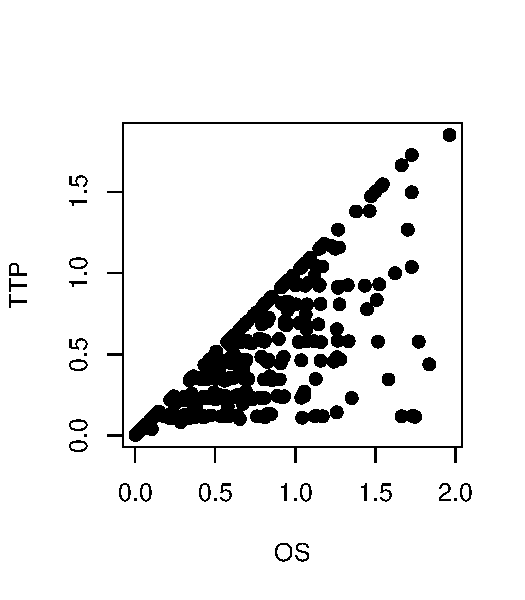
\includegraphics[width=0.31\textwidth]{chapters/figures/scatterplot.pdf}}\label{fig:scatter}
\subfloat[]{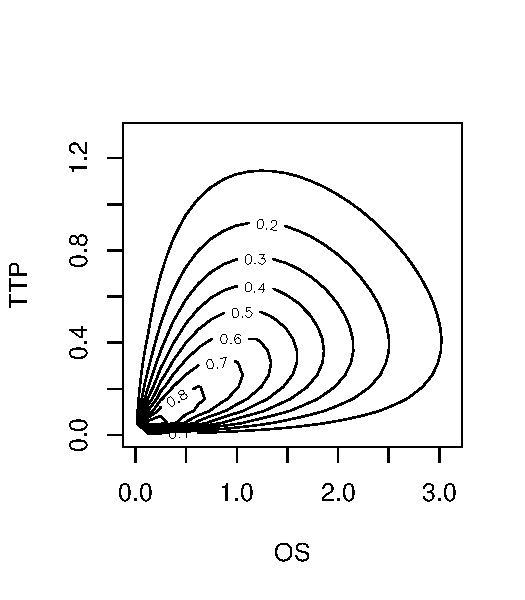
\includegraphics[width=0.325\textwidth]{chapters/figures/contour.pdf}}\label{fig:contour}
\subfloat[]{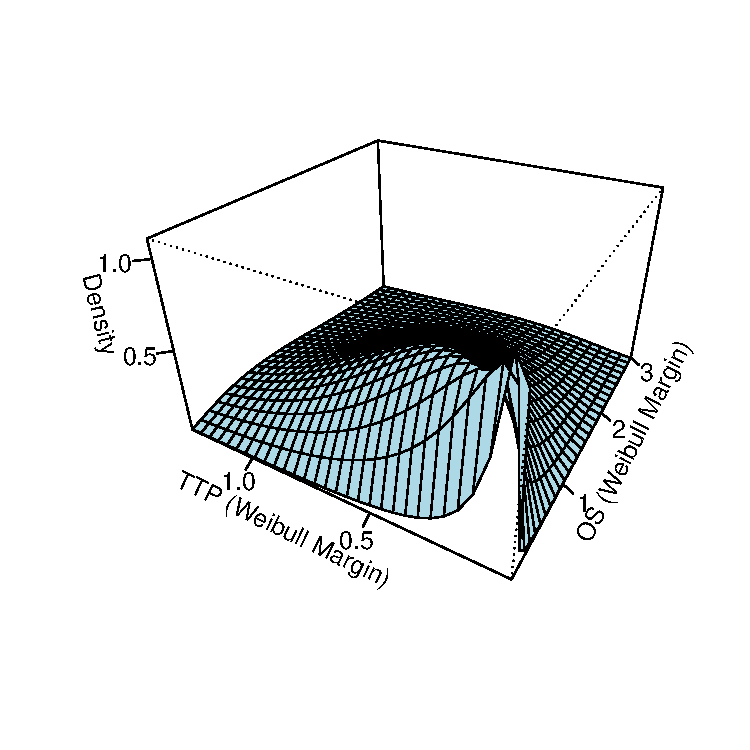
\includegraphics[width=0.35\textwidth]{chapters/figures/surface.pdf}}\label{fig:surface}
\caption{(a) The scatterplot between TTP and OS, (b) the contour plot of TTP vs. OS fitted with a Clayton copula, (c) the surface plot of TTP vs. OS fitted with a Clayton copula. \label{fig:copula}}
\end{figure}

\subsection{Standard Statistical Analysis}\label{sec:method_standard}

Most commonly, \ac{PFS} is modeled using a Kaplan-Meier curve or Cox regression. For example, just like what we discussed previously in Section \ref{sec:marginal}, a simple Weibull baseline hazard model has the form
$\lambda(t)=\alpha \gamma t^{\alpha-1} \exp(\textbf{Z}' \boldsymbol{\beta})$,
where $\textbf{Z}_i$ is the covariate matrix for modeling PFS, $\alpha$ and $\gamma$ are the shape and scale parameters of the Weibull distribution, and $\boldsymbol{\beta}$ is the vector of coefficients. Note that a standard analytic method does not consider the dynamics of the component processes of \ac{PFS} and does not take random effects into account.

\subsection{Prediction}

\subsubsection{Posterior Predictive Distribution (PPD)}
Within each of the models outlined in Sections \ref{sec:method_standard} through \ref{sec:jm}, we utilize the \ac{PPD} technique \citep{gelman2014bayesian} to generate \ac{OS} predictions. The \ac{PPD} represents the distribution of potential unobserved values based on the observed values, and it follows this structure:
$p(y_{pred}|y) = \int{p(y_{pred},\theta|y)d\theta} = \int{p(y_{pred}|\theta,y)p(\theta|y)d\theta} = \int{p(y_{pred}|\theta)p(\theta|y)d\theta}$,
This formulation leverages the conditional independence between $y$ (observed data), $y_{pred}$ (unobserved data), and $\theta$ (parameters). The \ac{PPD} can be understood as an average of conditional predictions over the posterior distribution of $\theta$. During the \ac{MCMC}  process, for each sampled $\theta$ from the posterior distribution, a corresponding $y_{pred}$ sample is obtained. To produce \ac{PPD} samples for \ac{OS} using the survival time modeling methods discussed, we used the \texttt{JAGS} software \citep{plummer2017jags} along with the \texttt{rjags} package for implementation in the R environment.

\subsubsection{Bayesian Model Averaging (BMA)}
In Section \ref{sec:jm}, we have established the three models governing the relationships between the target lesion, non-target lesion, new lesion, and OS, along with the marginal model for \ac{OS} in our joint model, a \ac{BMA} approach can be adopted to link all four models under the multivariate joint modeling approach together, enhancing the overall prediction capability.

In prognostic modeling, it is standard to generate predictions by selecting a single model based on certain metrics. In the context of oncology, different \ac{PFS} components may be more correlated with \ac{OS} under various tumor types or patient groups, thus offering more accurate \ac{OS} predictions. Here, we use \ac{BMA} to calculate the weighted average of the predicted \ac{OS} under the three joint models and one marginal model for \ac{OS} defined above. The weights indicate the plausibility of each model being the most predictive model. We denote the models defined in Section \ref{sec:TL}, \ref{sec:NT}, \ref{sec:NL}, and \ref{sec:marginal} by $M_T$, $M_{NT}$, $M_{NL}$, and $M_{OS}$, respectively. Then by BMA, the final predicted probability of \ac{OS} follows
\begin{align*}
P(Y_{pred}|Data)&=P(Y_{pred.t}|M_T,Data)P(M_T|Data)\\
&+P(Y_{pred.nt}|M_{NT},Data)P(M_{NT}|Data)\\
&+P(Y_{pred.nl}|M_{NL},Data)P(M_{NL}|Data)\\
&+P(Y_{pred.os}|M_{OS},Data)P(M_{OS}|Data),
\end{align*}
where $P(M_T|Data)$, $P(M_{NT}|Data)$, $P(M_{NL}|Data)$, and $P(M_{OS}|Data)$ are the model weights. In general, if we have a total of $Q$ models, the model weight for model $q$ at the $t$th \ac{MCMC}  iteration is  
$$w^{(t)}_q=P(M_q|Data,\theta^{(t)})=\frac{P(M_q,Data,\theta^{(t)})}{P(Data,\theta^{(t)})} =\frac{P(Data|M_q,\theta^{(t)})P(\theta^{(t)}|M_q)P(M_q)}{P(Data,\theta^{(t)})},$$
where $\theta^{(t)} = (\theta_1^{(t)}, \theta_2^{(t)},...,\theta_Q^{(t)})$. If we set $P(\theta_h|M_h, Data)=g_h$, and $q \ne h$, then according to \cite{congdon2007model},
$$P(\theta^{(t)}|M_q)=P(\theta_q^{(t)}|M_q) \prod_{h=1,h\ne q}^Q P(\theta_h^{(t)}|M_q)=P(\theta_q^{(t)}|M_q) \prod_{h=1,h\ne q}^Q g_h.$$
Therefore, 
$$w^{(t)}_q=P(M_q|Data,\theta^{(t)})=\frac{P(Data|M_q,\theta^{(t)}) P(\theta_q^{(t)}|M_q) \prod_{h=1,h\ne q}^Q g_h P(M_q) }{\sum_{k=1}^Q P(Data|M_k,\theta^{(t)}) P(\theta_k^{(t)}|M_k) \prod_{h=1,h\ne k}^K g_h P(M_k)}.
$$
We implement the \ac{BMA} approach using the above formula and calculate the final predicted OS. 



\subsection{Prior Specification}

In this section, we provide recommendations for specifying priors for the parameters in the models discussed in Section \ref{sec:method}. Our aim is to promote the use of generalizable, weakly informative, or non-informative priors for all model parameters to ensure robust and interpretable results. We also emphasize the importance of selecting appropriate priors to maintain parameter identifiability.

\subsubsection{General Guidelines}

For the $\boldsymbol{\beta}$ vector of coefficients, we recommend using weakly informative normal distributions with a mean of 0. We suggest weakly informative exponential distributions for the shape parameters ($\alpha$) in the Weibull distribution. All random effect parameters ($b$) should follow weakly informative normal distributions, denoted as $N(0, \sigma_{b_k}^2)$, where $k$ stands for different random variables under different copula models. Weakly informative half-normal priors are recommended for the standard deviations ($\sigma_{b_k}$) associated with the random effects. For all Clayton copula parameters ($\eta$), we recommend using weakly informative exponential distributions. These priors can accommodate a wide range of plausible values. In the following subsections, we provide recommendations for parameters specific to each model:

\subsubsection{Three-State Illness-Death Model}

In the Three-State Illness-Death Model, we advise using weakly informative half-normal priors for all $\Tilde{\gamma}$ parameters. These priors allow flexibility while constraining extreme values.

\subsubsection{Multivariate Joint Modeling Approach}

In the model assessing the association between target lesion and OS, which is a component of our proposed multivariate joint modeling approach, we suggest the following priors: For the parameter $\lambda$, a weakly informative normal distribution with a mean of 0 is recommended. The correlation coefficient ($\rho$) should have a non-informative prior, such as $Unif(-1, 1)$, to avoid biasing the estimation. Additionally, we assume that all 4 submodels are equally weighted before fitting BMA, that is, $P(M_q) = 1/Q$, for all $q = 1,...,Q$.


\section{Simulation}
\label{sec:simulation}

\subsection{Design}
We performed extensive simulations to evaluate the performance of the proposed multivariate joint modeling approach. All simulated datasets mimic the structure of the renal cell cancer trial data. Specifically, we assume 400 subjects and 25 visits. Longitudinal measurements of target lesion and new lesion status are recorded at each visit. For simplicity purposes, non-target lesion status is not included. Survival status is updated whenever deaths occur. The follow-up visits are scheduled for every two months within the first two years, then change to every three months until the end of the 5th year. We censor the subject's subsequent target lesion measurements and new lesion status whenever that subject's death occurs. In addition, we have assumed three scenarios: 1) \ac{OS} is independent of target lesion measurements and time to new lesion, 2) \ac{OS} is correlated with time to new lesion only, and 3) \ac{OS} is correlated with target lesion measurements only. In all scenarios, target lesion measurements and new lesion status are randomly and independently simulated, but \ac{OS} is generated under different conditions. Specifically, in scenario 1, \ac{OS} is randomly and independently simulated. In scenario 2, \ac{OS} is conditionally simulated from a bivariate copula model between \ac{OS} and new lesion status. Finally, in scenario 3, \ac{OS} is conditionally simulated based on the target lesion measurements. We assume a negative correlation between \ac{OS} and changes in tumor measurements. For each scenario, 100 datasets are generated. To simplify the simulation process, only $treatment$ is included in the covariate matrices. 

We compare predictions under four models: our proposed multivariate joint model (Section \ref{sec:jm}), a copula model for \ac{TTP} and OS (Section \ref{sec:method_copula}), a semi-markov three-state illness-death model \citep{weber2020statistical} (Section \ref{sec:multi-state}), and a marginal Weibull baseline hazard model of OS (Section \ref{sec:method_standard}). 

\begin{figure}
\centering
\subfloat[]{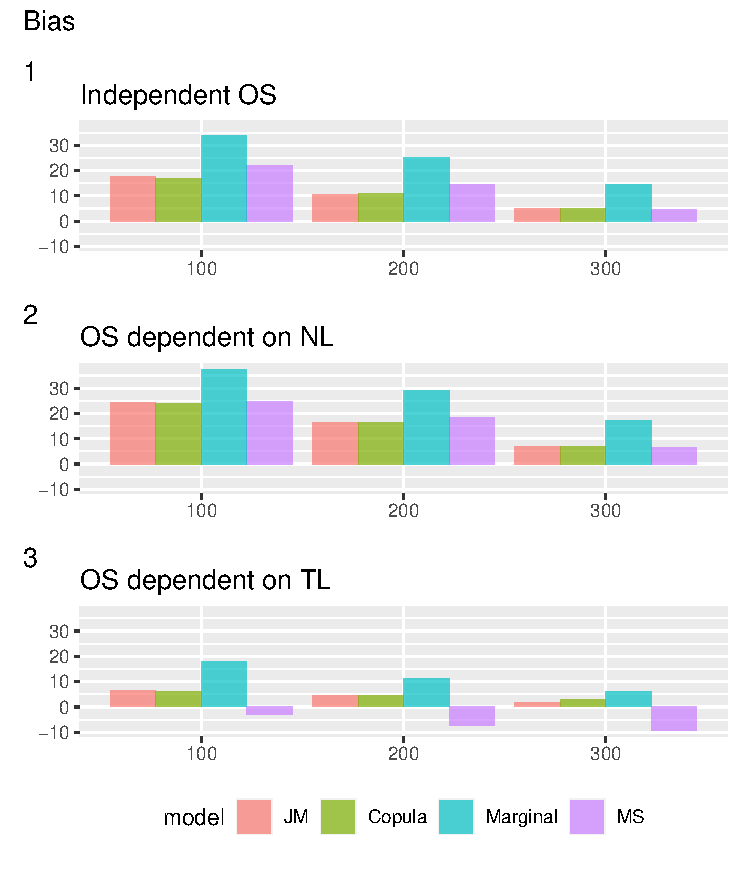
\includegraphics[width=0.5\textwidth]{chapters/figures/Bias.pdf}\label{fig:bias}}
\subfloat[]{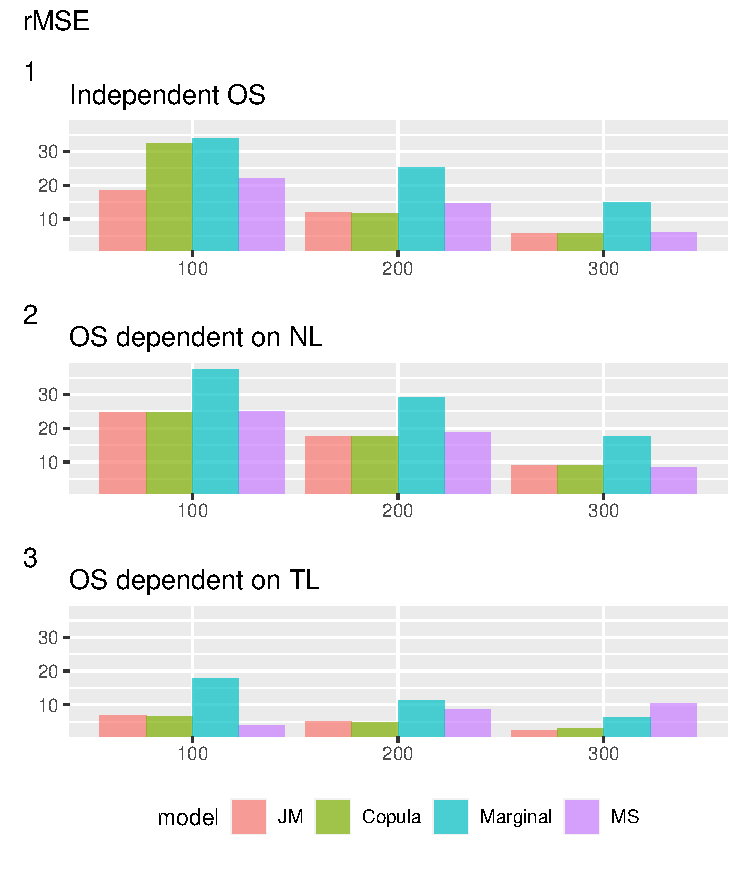
\includegraphics[width=0.5\textwidth]{chapters/figures/rMSE2.pdf}\label{fig:rmse}}
\caption{The bias (a) and rMSE (b) of the last death date predictors of four models: the multivariate joint modeling approach (JM), a copula model between PFS and \ac{OS} (Copula), the marginal Weibull baseline hazard model of OS (Marginal), and a three-state illness-death model (MS), under three OS scenarios. The $x$-axis denotes the number of death at cutoff. The $y$-axis denotes the number of months. \label{fig:result}}
\end{figure}



To emulate real trial scenarios and assess the prediction performance of our proposed method, we generate snapshots of the data such that for each simulated dataset, we have snapshots of what the data would have looked like if only 100, 200, and 300 death events had occurred. Then, we predict the time of the last (400th) death event under each snapshot dataset. Note that predictions may be performed at any time during the trial, and 100, 200, and 300 were selected for illustration purposes. Predictions from the four methods are compared. Finally, we calculate each predictor's \ac{CR}, \ac{rMSE}, bias, and width of the 90\% \ac{CI}. The 90\% \ac{CI} is the narrowest interval that includes 90\% of the posterior distribution of the predictor. 

\subsection{Results}

The bias and \ac{rMSE} of the predicted time of the last death are shown in Figures \ref{fig:bias} and \ref{fig:rmse}, and the corresponding \ac{CR} and \ac{CI} width are shown in Table \ref{tab:sim_result}. The weights of all submodels of the multivariate joint modeling approach under each simulation scenario are shown in Figure \ref{fig:weights_simulation}.

\begin{table}
\caption{The coverage rate (CR) and credible interval (CI) width for predictors of the time of the last death. Comparing the results from the multivariate joint modeling approach (JM), a copula model between PFS and OS (Cop), a three-state illness-death model (MS), and the marginal Weibull baseline hazard model of OS (Mrgl). The unit for CI width is month.  \label{tab:sim_result}}
\begin{center}
\begin{tabular}{ccccccccccccc}
& \multicolumn{4}{c}{Independent OS} & \multicolumn{4}{c}{OS dependent on NL} & \multicolumn{4}{c}{OS dependent on TL} \\ 
& JM & Cop & MS & Mrgl & JM & Cop & MS & Mrgl & JM & Cop & MS & Mrgl \\ \hline
\multicolumn{10}{l}{\textit{100 death event}}\\
CR & 0.49 & 0.49 & 0.01 & 0.00 & 0.11 & 0.11 & 0.03 & 0.00 &  0.91 & 0.91 & 1.00 & 0.00 \\ 
Width & 35.9 & 35.8 & 24.9 & 3.4  & 29.2 & 29.5 & 26.8 & 2.9  &  24.4 & 25.4 & 41.8 & 3.2 \\ \hline
\multicolumn{10}{l}{\textit{200 death event}}\\
CR & 0.89 & 0.86 & 0.33 & 0.00 & 0.45 & 0.45 & 0.24 & 0.00 & 0.85 & 0.98 & 1.00 & 0.00 \\ 
Width & 35.7 & 35.3 & 26.0 & 5.9 & 32.2 & 32.2 & 26.8 & 5.6 & 15.2 & 17.1 & 39.6 & 4.1  \\ \hline
\multicolumn{10}{l}{\textit{300 death event}}\\
CR & 0.98 & 0.98 & 0.98 & 0.00 & 0.90 & 0.89 &  0.95 & 0.01  & 0.97 & 0.98 & 1.00 & 0.00 \\ 
Width & 30.5 & 30.5 & 29.6 & 9.3 & 32.5 & 32.6 & 31.5 & 9.9 & 12.0 & 11.2 & 36.7 & 4.6 \\ 
\hline
\end{tabular}
\end{center}
\end{table}


\begin{figure}
\centering
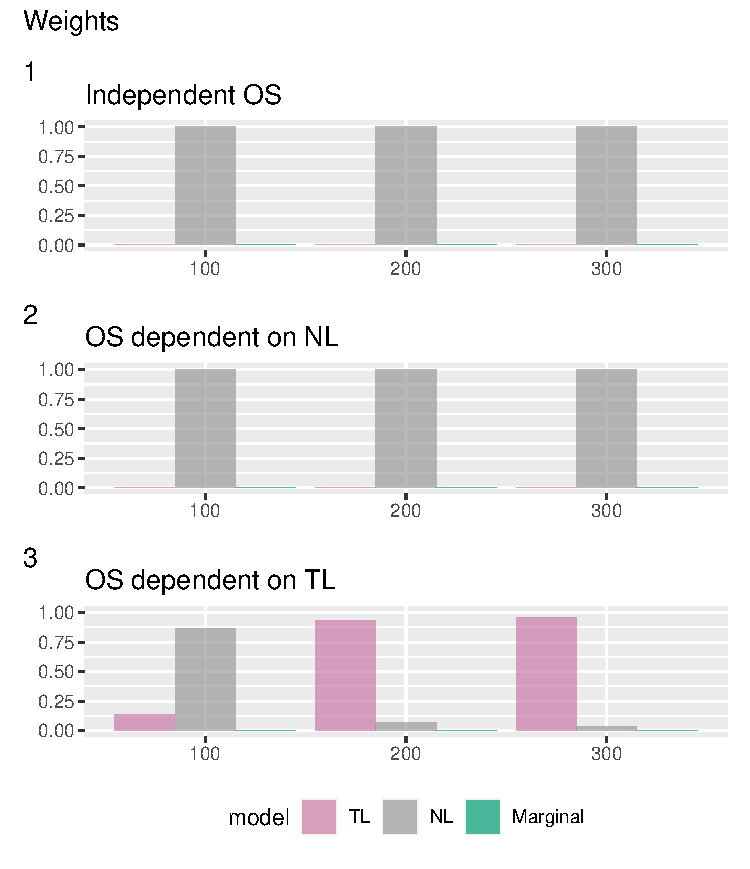
\includegraphics[width=8cm]{chapters/figures/Weights_simulation.pdf}
\caption{The weights of all submodels of the multivariate joint modeling approach for each snapshot dataset in the simulation studies.\label{fig:weights_simulation}}
\end{figure}

Under scenario 1, where \ac{OS} is generated independently, the bias and \ac{rMSE} of all predictors become smaller as we gather more information from the trial, i.e., more death events are observed. Overall, the marginal model performs worse than the other three models. This is likely due to the conservativeness of the Weibull model and the fact that it only utilizes \ac{OS} data, causing predictions to concentrate near the observed maximum OS. Given that the proposed model assigned all the weight to the copula model between new lesion and OS, it is reasonable that the copula model and the multivariate joint modeling approach have similar bias and \ac{rMSE}. Having evaluated all the metrics, the multivariate joint modeling approach and the copula model are the best-performing method under scenario 1.

In Scenario 2, where \ac{OS} is generated based on new lesion status, the multivariate joint modeling approach, the copula model, and the three-state illness-death model exhibit similar bias and \ac{rMSE} values. Once again, the marginal model lags behind the other models in performance. As with Scenario 1, as the number of observed death events increases, the bias and \ac{rMSE} of all predictors decrease. Compared to Scenario 1, the improved performance in bias and \ac{rMSE} of the three-state illness-death model can largely be attributed to the fact that the \ac{OS} observations generated under Scenario 2 more closely resemble a Weibull distribution. However, when only 100 or 200 death events are observed, the three-state illness-death model has a lower \ac{CR} than the other two. This might be due to the conservatives of the standard Weibull model. Consequently, for Scenario 2, we would still recommend either the joint modeling approach or the copula model.

In Scenario 3, where \ac{OS} is derived based on target lesion measurements, the proposed multivariate joint modeling approach begins to surpass the copula model as more death events are observed. Simultaneously, as the count of observed death events increases, the multivariate joint modeling approach assigns greater weight to the joint model between the target lesion and OS, which is anticipated. This is expected as the multivariate joint modeling approach is the only method that captures the relationship between \ac{OS} and the target lesion. Differing from the other two scenarios, the bias and \ac{rMSE} of predictors from the three-state illness-death model do not consistently diminish with the increase in observed death events. Moreover, the three-state model displays the widest \ac{CI} among all the models. This can be attributed to the alteration in \ac{OS} distributions, as it is generated based on the target lesion distribution, which does not conform to a Weibull distribution. The inflexibility of the standard Weibull baseline hazard model, devoid of random effects, further contributes to this.

According to Figure \ref{fig:result}, across all scenarios, the proposed multivariate joint modeling approach performs either the best or very similar to the copula model, if the copula model is the best-performing one. This is reasonable as the \ac{BMA} could assign $w_q = 1$ to submodel $q$ when submodel $q$ is significantly better than the other $q-1$ submodels. If this is the case, the multivariate joint modeling approach predictions will be the same as the predictions from its submodel $q$. The multivariate joint modeling approach and the copula model are less sensitive to changes in the \ac{OS} distribution and still provide relatively reasonable predictions even when \ac{OS} prediction does not closely resemble a Weibull distribution. In summary, the multivariate joint modeling approach provides the most reliable predictions across all tested scenarios.

\begin{figure}
\centering
\subfloat[]
{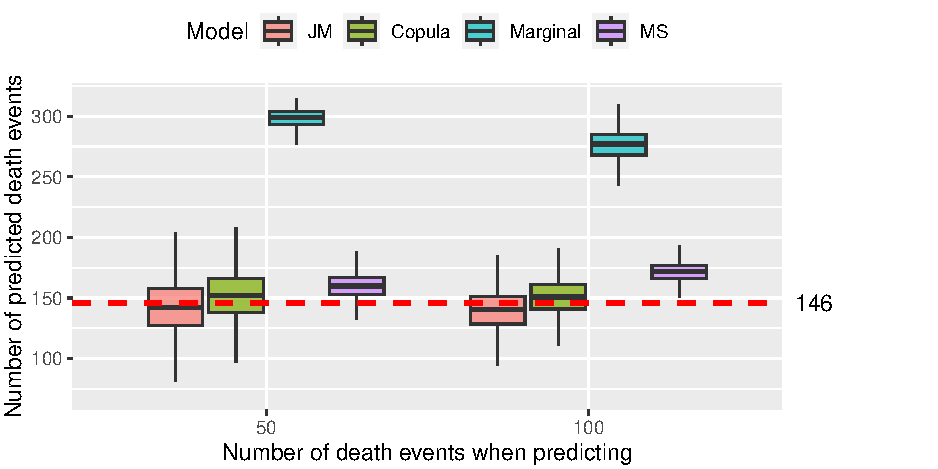
\includegraphics[width=0.74\textwidth]{chapters/figures/primary_analysis.pdf}\label{fig:primaryanalysis}}
\hfill
\subfloat[]
{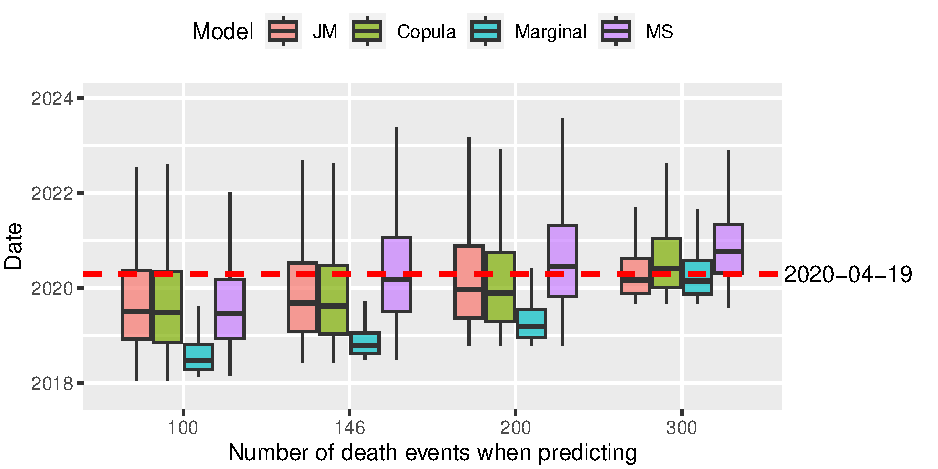
\includegraphics[width=0.74\textwidth]{chapters/figures/lastdeath1.pdf}\label{fig:casestudy}}
\hfill
\subfloat[]
{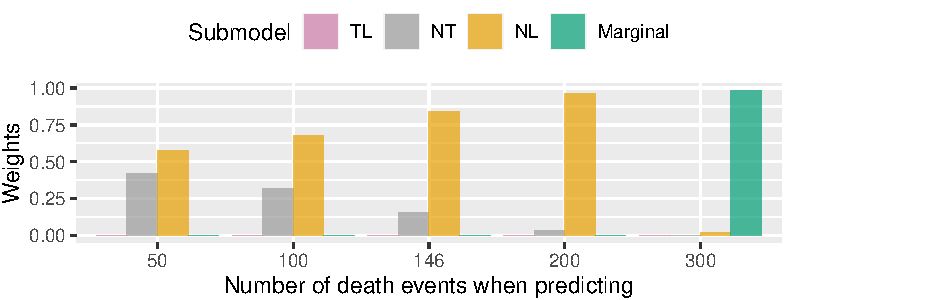
\includegraphics[width=0.74\textwidth]{chapters/figures/weights.pdf}\label{fig:weights}}
\caption{(a) Boxplots of the posterior distributions of the last death date by the proposed multivariate joint modeling approach, the copula model between PFS and OS, the marginal Weibull baseline hazard model of OS, and the three-state illness-death model. Date ``2020-04-19" is the true last death date. (b) The final weights of each submodel under the proposed multivariate joint modeling approach. (c) The weights of all submodels of the multivariate joint modeling approach for each recreated dataset.}
\end{figure}

\section{Analysis of the Renal Cell Carcinoma Data}
\label{sec:caseanalysis}
We return to the renal cell carcinoma dataset introduced in Section \ref{sec:example}. Our objective here is to predict the timing of the last death in this clinical trial by fitting the multivariate joint model we developed in Section \ref{sec:jm} to all available tumor measurements. We generate snapshots of the trial data at the 100th, 146th (the time of primary analysis), 200th, and 300th death, and compare predictions under four models: the multivariate joint model, a copula model for \ac{TTP} and OS, a three-state illness-death model, and a marginal model of OS. 

We included \textit{gender, age, nephrectomy at baseline, Heng prognostic criteria at baseline, and ECOG Performance Status} into the covariates matrix $\textbf{X}_i$ and $\textbf{Z}_i$. Then, we fit each model using two \ac{MCMC}  chains, each with at least 10,000 \ac{MCMC}  iterations, 1,000 burn-in, and 8,000 adaptation iterations.  Convergence diagnostic tests and autocorrelation plots did not show any alarming indications of convergence failure. Figure \ref{fig:primaryanalysis} displays the predicted number of deaths at the time of the primary analysis. Figure \ref{fig:casestudy} presents boxplots of the posterior distributions for the predictors of the last death date from all tested models compared to the true last death date. The median values of the boxplots serve as point predictions. Figure \ref{fig:weights} displays the weights of all submodels for each recreated dataset. In this specific case study, the new lesion is observed to have the strongest correlation with OS. Therefore, it makes sense that greater weights are assigned to the new lesion copula submodel, and the copula model between \ac{TTP} and \ac{OS} also performs well. While the marginal model exhibits significantly smaller \ac{CI}s, its predictors prove to be less accurate than those of the multivariate joint modeling approach and the copula model, especially when we observe 100, 146, and 200 deaths. These latter models consistently demonstrate the most reliable performance improvements as the number of observed deaths increases. When we have 300 deaths observed and the marginal model performs the best among all submodels, the \ac{BMA} procedure naturally assigns more weight to it, as indicated in Figures \ref{fig:casestudy} and \ref{fig:weights}. Considering that the posterior samples of the three-state illness-death model are derived by combining predictions from two distinct time periods - randomization to progression and progression to death — it is reasonable for the three-state model to exhibit the widest \ac{CI}s. 

\begin{table}
\caption{Bias and \ac{rMSE} of the predictors of multivariate joint modeling approach (JM), copula model, marginal model, and three-state illness-death model (MS). \label{tab:casestudytable}}
\begin{center}
\begin{tabular}{ccccccc}
\hline
\multicolumn{2}{c}{No. of events} & \multirow{2}{*}{Metric} & \multirow{2}{*}{JM} & \multirow{2}{*}{Copula} & \multirow{2}{*}{Marginal} & \multirow{2}{*}{MS}\\ 
Observed & Predicted & & & & & \\\hline
\multirow{2}{*}{100} & \multirow{2}{*}{241} & Bias & 0.67 & 1.71 & 9.46 & 1.35\\
&& rMSE & 3.71 & 3.94 & 10.56 & 3.73 \\ \hline
\multirow{2}{*}{146} & \multirow{2}{*}{195} & Bias & 1.41 & 2.11 & 9.13 & 2.54\\
&& rMSE & 2.56 & 3.13 & 9.65 & 3.14 \\ \hline
\multirow{2}{*}{200} & \multirow{2}{*}{141} & Bias & 0.91 & 2.15 & 7.89 & 3.11\\
&& rMSE & 2.06 & 2.91 & 8.19 & 3.65 \\ \hline
\multirow{2}{*}{300} & \multirow{2}{*}{41} & Bias & 6.23 & 2.97 & 6.32 & 4.13  \\
&& rMSE & 8.24 & 6.14 & 8.28 & 7.31  \\ \hline
\end{tabular}
\end{center}
\end{table}

Table \ref{tab:casestudytable} presents the bias and \ac{rMSE} of the predicted \ac{OS} when 100, 146, 200, or 300 death events are observed. In the first three scenarios, the multivariate joint modeling approach performs similarly to the copula model and the three-state model. In the last scenario, the joint model performs similarly to the marginal model, consistent with the submodel weights shown in Figure \ref{fig:weights}. Additionally, the joint model exhibits smaller bias and rMSEs compared to the marginal model under all scenarios. While the multivariate joint modeling approach may not always have the smallest bias in this particular case study dataset, its prediction reliability is consistently verified. 

We used all four models to forecast the \ac{OS} of patients with censored \ac{OS} in the case study data set. Subsequently, we generated predicted Kaplan-Meier plots for each model (Figure \ref{fig:predictionKM}). Finally, we estimated the potential gain or loss in life expectancy by calculating the difference in the area under the curve between the experimental drug and the standard of care \citep{pak2017interpretability, survRM2}. The results from Figure \ref{fig:predictionKM} indicate that all models consistently project a substantial improvement in life years. In addition, the multivariate joint modeling approach and the copula model, whose reliability was previously established in this case study, both forecast a roughly 7.5-month gain in life years for patients who receive the experimental drug, as opposed to the standard of care.


\section{Discussion}
\label{sec:discussion}
In this paper, we were motivated by an advanced renal cell carcinoma clinical trial to present how real-time \ac{OS} predictions from joint models with different components of \ac{PFS} can be dynamically combined via BMA. This multivariate joint modeling approach provides reliable estimates of the time of the $n$th death in a trial using all available tumor assessment data based on \ac{RECIST} 1.1. This is valuable for clinical trial planning and patients' end-of-life medical care. Furthermore, the proposed multivariate joint model method provides the most reliable and robust predictions in the case study and across all the scenarios we tested in the simulation studies. This approach can be easily applied to other solid tumor types beyond renal cell carcinoma.

\begin{figure}[H]
    \centering
    \subfloat[]{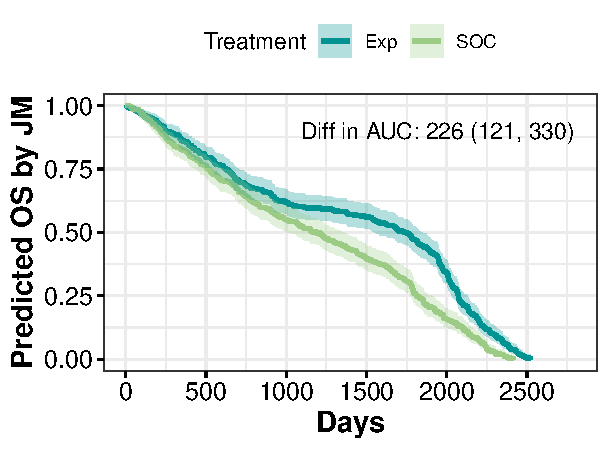
\includegraphics[width=0.49\textwidth]{chapters/figures/JMprediction.pdf}\label{fig:JMprediction}}
    \subfloat[]
    {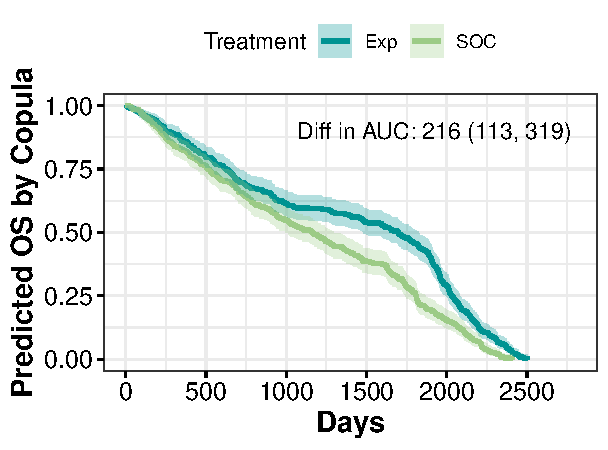
\includegraphics[width=0.49\textwidth]{chapters/figures/copulaprediction.pdf}\label{fig:Copulaprediction}}
    \hfill
    \subfloat[]{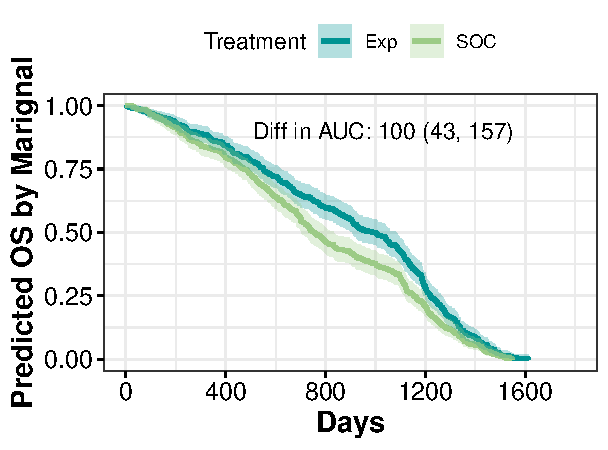
\includegraphics[width=0.49\textwidth]{chapters/figures/marginalprediction.pdf}\label{fig:Marginalprediction}}
    \subfloat[]{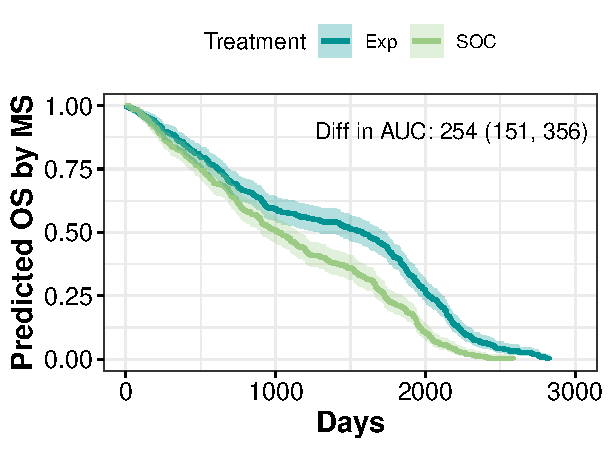
\includegraphics[width=0.49\textwidth]{chapters/figures/MSprediction.pdf}\label{fig:MSprediction}}
    \caption{Kaplan-Meier plots of the observed and predicted overall survival by the multivariate joint modeling approach (a), the copula model(b), the marginal model (c), and the three-state illness-death model. The difference in the area under the curve (AUC) and its CIs for the experimental drug (Exp) and the standard of care (SOC) are also included.}
    \label{fig:predictionKM}
\end{figure}

The multivariate joint modeling approach is flexible and can easily incorporate a linear model with time-dependent covariates or a nonlinear mixed-effects model. Although \ac{BMA} methods optimally combine multiple models, they typically require extended training time due to their complexity. In the example data analysis, only five covariates were included. Incorporating additional baseline characteristics is possible, but doing so would expand the covariate matrix and further increase the computational demands of the multivariate joint modeling approach. Considering that the covariates utilized in each submodel may vary, it is beneficial to determine the most suitable covariates for each submodel before implementation. This covariates selection process can be guided by expert opinion or variable selection models, potentially reducing the covariate matrix's size.

Based on the simulation studies and the example data analysis, it is evident that the copula model for \ac{TTP} and \ac{OS} ranks as the second most reliable model among all those tested. If the \ac{TTP} and \ac{OS} data are well-fitted by Weibull distributions with random effects, the copula model typically performs better than the marginal \ac{OS} model. Therefore, fitting only a copula model with random effects is an excellent option to reduce model training time. Based on our simulations, without including random effects, high variability between individuals will cause the copula model's predictions to be too heavy-tailed.

For a marginal \ac{OS} model to perform better, it would be beneficial to incorporate more predictive covariates or use a model offering greater flexibility than the Weibull baseline hazard model, such as parametric regression models. Similarly, to improve the performance of the multi-state model, we could replace the Weibull baseline hazard model with more flexible models.

During the simulation studies, the data for non-target lesions was not simulated, yet it was included in the example data analysis. This does not undermine the outcome of our simulation studies, given that both the non-target lesion and new lesion were modeled using the exact same joint model, and each component of \ac{PFS} was modeled separately. If the non-target lesion data had been included in the simulation dataset, we would anticipate longer training times for the multivariate joint modeling approach without observing any relative improvement in performance given the scenarios we defined.

Apart from applying the same model weights for all the patients in the dataset, \ac{BMA} can potentially provide personalized model weights, i.e., for different patients, different models may have higher weights. This could further improve the prediction accuracy. Future work can explore how to implement personalized model weights in a time-efficient manner under the setting of this study.
% Place your additional chapters here using the \input{} command
\chapter{Integrating External Control Data at the Patient Level into the Longitudinal Small Sample, Sequential, Multiple Assignment Randomized Trial (snSMART) Design}
\label{chpt:chpt4}

\section{Research Plan}
In this project, we plan to present a study design that builds upon the trial design outlined in Chapter II by incorporating longitudinal data collected at each stage. Our goal is to estimate the stage 1 treatment effect more efficiently by utilizing longitudinal data from both stages of the trial and incorporating external data. This design will be particularly advantageous as it allows for the inclusion of a larger amount of data from natural history studies that are collected over time. To evaluate the treatment effect in our proposed study design, we plan to employ a Bayesian mixed model for repeated measures (MMRM) and account for confounding variables through inverse probability treatment weighting (IPTW). MMRM is a statistical model that facilitates the analysis of repeated measures data and takes into account the correlation between measurements taken on the same subject. IPTW is a technique that helps to balance the distribution of covariates between the treatment groups, thus reducing bias caused by confounding variables. Additionally, we will derive a robust Meta-Analytic Predictive (MAP) \citep{schmidli2014robust} prior for the model intercept of the Bayesian MMRM using the IPTW-adjusted pseudo population of external control data. The MAP approach allows for further down-weighting of external control data if there is a higher degree of variability between data sources. This approach allows us to consider various sources of heterogeneity and potential selection bias when combining external control data and data from different stages of the trial. To evaluate the performance of our proposed method, we will conduct simulation studies comparing it to traditional analytic methods. These simulations will provide insight into the strengths and limitations of our approach and help to identify the conditions under which it performs well.

\section{Literature Review}
The papers reviewed here focus on the use of statistical models in the analysis of disease progression in progressive rare diseases such as centronuclear myopathy, Duchenne muscular dystrophy (DMD), and GNE myopathy. These papers also discuss the use of Bayesian modeling in the analysis of clinical trial data and the incorporation of external data into the analysis.

In the paper by \cite{raket2022progression}, a novel progression model called progression models for repeated measures (PMRMs) is introduced. The purpose of this model is to estimate non-traditional treatment effects, such as slowing or delaying the progression of a disease. PMRMs combines linear mixed effects models and penalized splines, providing better interpretability and clinically relevant insights through the analysis of time-based treatment effects.

\cite{fouarge2021hierarchical} adopted a hierarchical Bayesian mixed-effects model to study the progression of centronuclear myopathy. By incorporating random effects for each patient, the model was able to capture the variations in the level and progression of the disease among individuals. This approach enabled the comparison of the outcomes of patients at a specific time post-treatment to simulated endpoint scores without treatment, providing valuable insights for rare disease trial analysis.

\cite{lennie2020latent} propose a latent process model to investigate the progression of Duchenne Muscular Dystrophy (DMD) using the 6-minute walk test (6MWT) results. The model is a single continuous structural model with a single covariance matrix for random variability across all subjects. By using this model, the authors aim to estimate the rate of disease progression in patients with DMD and predict patients' 6MWT scores.

\cite{quintana2019bayesian} used a Bayesian approach to analyze data collected longitudinally from GNE myopathy patients. The focus of the study was on the patients' muscle strength, which was used to develop a Bayesian Disease Progression Model (DPM). The DPM aligns subjects based on a latent disease age, and provides prediction of future long-term disease progression for each subject conditional upon the subject-level disease age and inherent muscle strength. 

\cite{zhou2021incorporating} propose a method for incorporating external data into the analysis of clinical trials via Bayesian additive regression trees (BART), with a specific goal of estimating the conditional or population average treatment effect. BART adaptively pools information across data sources to improve the precision of treatment effect estimations. 

\cite{kiran2021bayesian} propose a new method for creating synthetic control groups in clinical trials using a Bayesian nonparametric mixture model. This approach utilizes electronic health records (EHR) to identify similar population segments. The synthetic control group can then be used to make inferences about treatment effects using standard methods for randomized controlled trials (RCT).

Overall, these papers highlight the use of statistical models and Bayesian modeling in the analysis of disease progression in progressive diseases and the incorporation of external data into the analysis of clinical trial data. 

In addition, these papers demonstrate the importance of incorporating individual variation and external data into the analysis of disease progression. By accounting for individual variations, these models can provide a more accurate understanding of disease progression and inform personalized treatment options. Incorporating external data allows for the analysis of larger and more diverse datasets, which can improve the generalizability of the results. Our method is specific for the snSMART design and there differs from the papers discussed above. 

Our proposed method for this research project, combining IPTW, Bayesian MMRM, and MAP, will provide a new way to consider both individual variations and external control data simultaneously. 

\section{External Control Data}
We have requested access to the below DMD datasets and will use them to conduct case studies in our Chapter IV project.
\begin{itemize}
    \item Duchenne Natural History Study (DNHS) - Cooperative International Neuromuscular Research Group (CINRG). \url{https://clinicaltrials.gov/ct2/show/NCT00468832}
    \item A Prospective Natural History Study of Progression of Subjects With DMD - BioMarin Pharmaceutical \url{https://clinicaltrials.gov/ct2/show/NCT01753804}
    \item A Study of Tadalafil for DMD - Eli Lilly and Company \url{https://clinicaltrials.gov/ct2/show/NCT01865084}
    \item Natural history study by Cincinnati Children's Hospital Medical Center (CCHMC) (2004–2016)
    \item Magnetic Resonance Imaging and Biomarkers for Muscular Dystrophy - University of Florida \url{https://clinicaltrials.gov/ct2/show/NCT01484678}
\end{itemize}
% Place your additional chapters here using the \input{} command
\chapter{Conclusion}
\label{chpt:conclusion}



% Appendices
\appendix
\input{appendices/example_appendix_01}
\input{appendices/example_appendix_02}

\bibliographystyle{agsm}

% Give this command the relative path to the .bib file.
\bibliography{references.bib}

\end{document}
